\documentclass[12pt,a4paper]{article}
\usepackage[utf8]{inputenc}
\usepackage[T1]{fontenc}
\usepackage[spanish,es-tabla]{babel}
\usepackage{lmodern,microtype,amsmath,amssymb,graphicx,booktabs,longtable,array,pdflscape,caption,xcolor,listings,fancyhdr,geometry,enumitem,needspace}
\geometry{left=2.5cm,right=2.5cm,top=2.4cm,bottom=2.4cm}
\usepackage[hidelinks]{hyperref}
\usepackage{xurl}
\setlength{\parindent}{0pt}
\setlength{\parskip}{5pt}
\emergencystretch=2em
\setlength{\headheight}{16pt}
\setlength{\tabcolsep}{3pt}
\renewcommand{\arraystretch}{1.08}
\definecolor{azul}{HTML}{173D5C}
\definecolor{backcolour}{rgb}{.95,.95,.92}
\definecolor{codegreen}{rgb}{0,.6,0}
\definecolor{codegray}{rgb}{.5,.5,.5}
\definecolor{codepurple}{rgb}{.58,0,.82}
\lstdefinestyle{mystyle}{backgroundcolor=\color{backcolour},commentstyle=\color{codegreen},keywordstyle=\color{magenta},numberstyle=\tiny\color{codegray},stringstyle=\color{codepurple},basicstyle=\ttfamily\footnotesize,breaklines=true,captionpos=b,keepspaces=true,numbers=left,numbersep=5pt,showstringspaces=false,tabsize=2,columns=fullflexible}
\lstset{style=mystyle}
\captionsetup{font=small,labelfont=bf}
\renewcommand{\refname}{}
\pagestyle{fancy}\fancyhf{}\lhead{\small Algoritmos de Ruteo}\rhead{\small Path Discovery}\cfoot{\thepage}
\hypersetup{pdftitle={Tarea individual: Path Discovery},pdfauthor={Diego Muñoz}}
\begin{document}
\begin{titlepage}\centering
\vspace*{2cm}
{\Large Algoritmos de Ruteo\par}\vspace{1.5cm}
{\Huge\bfseries\color{azul} Tarea individual\par}\vspace{.5cm}
{\LARGE Path Discovery\par}\vspace{.6cm}
{\large Comparación de Scamper y RIPE Atlas\par}
\vfill
{\large Integrante: Diego Muñoz\par}\vspace{.5cm}
{\large Profesor: Nicolas Boettcher\par}
\vfill
{\large 27 de octubre de 2026\par}
\vspace{.6cm}
{\small Banda ancha fija domiciliaria WOM, Quilicura, Chile\par}
\end{titlepage}
\pagenumbering{roman}\tableofcontents\clearpage
\pagenumbering{arabic}
\clearpage
\section{Introducción}\label{sec:intro}
Este trabajo caracteriza las rutas de Internet utilizadas desde una conexión de banda ancha fija domiciliaria y compara la información revelada por Scamper y RIPE Atlas. Las preguntas son qué método descubre más interfaces por destino, qué cambia al invertir el sentido y qué patrones permiten reconocer las sondas en una captura.

El objetivo es documentar observaciones reproducibles y su alcance. Una IP de respuesta representa una interfaz observada; no equivale por sí sola a un router físico. Los ASN se obtienen de asociaciones IP-prefijo y no constituyen una ruta BGP medida.

\subsection{Conexión de origen}
\begingroup
\fontsize{9}{11}\selectfont
\addtocounter{table}{-1}
\begin{longtable}{p{4.2cm}p{10.3cm}}
\toprule
\textbf{Dato} & \textbf{Valor} \\ \midrule
\endfirsthead
\toprule
\textbf{Dato} & \textbf{Valor} \\ \midrule
\endhead
Proveedor comercial & WOM, confirmado por el estudiante \\
Ubicación aproximada & Quilicura, Región Metropolitana de Chile \\
IPv4 pública & 186.189.89.115 \\
Prefijo & 186.189.89.0/24 \\
ASN & AS52341 \\
Sonda local & 1018487 \\
Interfaz & wlan0 \\
\bottomrule
\end{longtable}
\endgroup
La asociación IP-prefijo-AS proviene de RIPEstat y sus respuestas conservadas. La consulta en BGP HE del 27 de octubre de 2026 confirma AS52341 (WOM S.A.) y muestra los anuncios 186.189.80.0/20 y 186.189.89.0/24; se usa el más específico. Su captura y transcripción se incluyen en los anexos y en el manifiesto de fuentes. Las direcciones privadas y 100.88.0.1 observadas son compatibles con NAT; sin comprobar la WAN del router no se confirma CGNAT.

\subsection{Destinos y motivación}
\begingroup
\fontsize{9}{11}\selectfont
\addtocounter{table}{-1}
\begin{longtable}{p{3cm}p{6cm}p{3cm}}
\toprule
\textbf{Destino} & \textbf{IPv4} & \textbf{Sonda} \\ \midrule
\endfirsthead
\toprule
\textbf{Destino} & \textbf{IPv4} & \textbf{Sonda} \\ \midrule
\endhead
Valparaíso & 138.204.230.242 & 6652 \\
La Habana & 200.14.48.134 & 12734 \\
Rusia & 37.79.226.46 & 3959 \\
\bottomrule
\end{longtable}
\endgroup
Se usan las alternativas admitidas por el enunciado actualizado. Valparaíso, La Habana y Rusia son los casos propuestos por el curso para contrastar contextos de conectividad. Las referencias del enunciado a velocidad y censura motivan la selección, pero estos traceroutes no miden velocidad de acceso ni demuestran censura. El destino ruso anterior, 90.150.251.81 / 870, se conserva como antecedente y queda fuera del análisis vigente. Se consideran tres destinos; la referencia del punto 4 a sí mismo se interpreta como una referencia al proceso bidireccional del punto 3.

\noindent Fuentes para la conexión de origen: RIPEstat \cite{ref4} y BGP HE \cite{ref7}; la motivación y los destinos proceden del enunciado \cite{ref8}.


\clearpage
\section{Metodología}\label{sec:metodo}
\subsection{Entorno y herramientas}
Equipo Linux CachyOS en la conexión WOM domiciliaria. Scamper 20260902, sus conversores y las herramientas de captura se ejecutaron con Docker Compose. La sonda RIPE Atlas usa red del host, identidad persistente y una imagen fijada por digest. La versión y la configuración efectiva se conservan por ejecución. Las capturas se inspeccionaron en Wireshark 4.6.6 y se exportaron con TShark.

Antes y después de cada ejecución se verificó la IPv4 pública esperada. El piloto contrastó WARTS, JSON, puertos, solicitudes emitidas y citas ICMP. Las mediciones relacionadas se ejecutaron secuencialmente, sin campañas locales superpuestas.

\subsection{Diseño de mediciones}
\begingroup
\fontsize{9}{11}\selectfont
\addtocounter{table}{-1}
\begin{longtable}{p{10cm}p{2cm}p{2cm}}
\toprule
\textbf{Familia} & \textbf{Por ronda} & \textbf{Tres rondas} \\ \midrule
\endfirsthead
\toprule
\textbf{Familia} & \textbf{Por ronda} & \textbf{Tres rondas} \\ \midrule
\endhead
Scamper trace: seis métodos x tres destinos & 18 & 54 \\
Scamper tracelb: cinco modos x tres destinos & 15 & 45 \\
RIPE ida: tres protocolos x tres destinos & 9 & 27 \\
RIPE vuelta: tres protocolos x tres destinos & 9 & 27 \\
Total & 51 & 153 \\
\bottomrule
\end{longtable}
\endgroup
Las rondas son repeticiones completas, distintas de los paquetes por salto. Las rondas rusas se separaron al menos 30 minutos desde el cierre anterior. Los dos primeros destinos pertenecen a una campaña anterior; no se presentan como una instantánea simultánea con Rusia. Tras un reinicio durante la primera ronda rusa, el intento incompleto y seis resultados previos se conservaron y se repitió esa ronda completa. Las comparaciones temporales se realizan dentro de cada destino.

\subsection{Sondas, puertos y comandos}
Scamper se limitó a 20 paquetes por segundo. TCP utilizó puerto de destino 80 y UDP base 33435, validada contra el piloto RIPE. RIPE mantuvo el resto de sus parámetros predeterminados y seleccionó sondas por ID exacto: 1018487 en ida y la sonda de cada destino en vuelta. Cada vuelta apuntó a 186.189.89.115. El apéndice conserva los comandos efectivos y las definiciones RIPE completas.

\begin{lstlisting}[caption={Forma de los comandos Scamper; los valores efectivos están en cada metadata.json.}]
scamper -p 20 -w 1 -O warts -o - \
  -c "trace -P METODO -d PUERTO" -i DESTINO
scamper -p 20 -w 1 -O warts -o - \
  -c "tracelb -P MODO -d PUERTO" -i DESTINO
# ICMP no necesita puerto de destino.
\end{lstlisting}
Métodos trace: UDP, ICMP, UDP-Paris, ICMP-Paris, TCP y TCP-ACK. Modos tracelb: UDP-dport, ICMP-echo, UDP-sport, TCP-sport y TCP-ack-sport. Las opciones específicas y los valores predeterminados son parte del procedimiento de cada algoritmo, no se asumen equivalentes por compartir protocolo.

\subsection{Captura, normalización y métricas}
Dumpcap guardó PCAPNG con un filtro de captura que incluyó ICMP y el destino. TShark separó solicitudes exteriores de las cabeceras originales citadas dentro de ICMP; se excluyeron paquetes RST de control al contar sondas TCP. En vuelta, la captura domiciliaria es parcial y no permite observar todos los paquetes emitidos remotamente.

La unidad normalizada es una respuesta por intento y TTL. Se preservan respuestas múltiples, errores y ausencias. En las tablas, * significa timeout registrado, ? significa que la herramienta no registró la respuesta y -- indica ausencia de registro para ese TTL en esa ejecución; no significa que no se haya ejecutado el método. [priv./esp.] indica dirección no global y [AS n/d] asociación no disponible. Un TTL 255 separado no se une artificialmente al salto anterior.

\begingroup
\fontsize{9}{11}\selectfont
\addtocounter{table}{-1}
\begin{longtable}{p{3cm}p{11.3cm}}
\toprule
\textbf{Métrica} & \textbf{Definición y uso} \\ \midrule
\endfirsthead
\toprule
\textbf{Métrica} & \textbf{Definición y uso} \\ \midrule
\endhead
IP únicas & Conjunto de direcciones de respuesta de cada ejecución; no es cantidad de routers físicos. \\
Cobertura & Proporción de TTL registrados con al menos una respuesta, según la normalización. \\
Estabilidad & Jaccard entre conjuntos de IP de rondas; conjuntos vacíos no prueban estabilidad perfecta. \\
Costo & Sondas informadas en WARTS y solicitudes observadas en PCAP; en RIPE inverso no se reconstruye emisión remota. \\
Elección & Mediana de IP únicas por destino; cobertura y estabilidad como desempates. \\
\bottomrule
\end{longtable}
\endgroup
Las tablas principales usan la ronda 2; las estadísticas usan las tres rondas. Se incluyen las rondas 1 y 3 en anexos. El descubrimiento con más paquetes se informa junto con ese costo, sin atribuir toda diferencia al algoritmo.

\subsection{Construcción y publicación de grafos}
Se eligió un par de ida/vuelta del mismo destino, protocolo, ronda e IPv4 de sesión. El criterio lexicográfico maximiza la unión de IP, minimiza huecos y minimiza separación temporal. Los grafos dirigidos conservan las referencias RIPE y distinguen interfaz, hueco y capa ambigua. Las aristas indican adyacencia inferida u orden de capas; no se forman productos cartesianos de respuestas múltiples. La publicación NDEx se comprobó sin credenciales y se conservó la copia exportada.

\noindent Bases documentales: Scamper \cite{ref1}; captura y exportación \cite{ref2}; mediciones RIPE \cite{ref3}; asociación de ASN \cite{ref4}; publicación y formato de grafos \cite{ref5,ref6}. Los detalles experimentales provienen de los originales locales.


\begin{landscape}
\section{Resultados y análisis}\label{sec:resultados}
\subsection{Path Discovery con Scamper}\label{sec:scamper}
\subsubsection{Valparaíso - 138.204.230.242}
\begingroup
\fontsize{9}{11}\selectfont
\begin{longtable}{p{0.95cm}p{3.725cm}p{3.725cm}p{3.725cm}p{3.725cm}p{3.725cm}p{3.725cm}}
\caption{Ruta observada con los seis métodos Scamper; Valparaíso, ronda 2.}\label{tabla1:138.204.230.242} \\
\toprule
\textbf{HOP} & \textbf{udp} & \textbf{icmp} & \textbf{udp-paris} & \textbf{icmp-paris} & \textbf{tcp} & \textbf{tcp-ack} \\ \midrule
\endfirsthead
\toprule
\textbf{HOP} & \textbf{udp} & \textbf{icmp} & \textbf{udp-paris} & \textbf{icmp-paris} & \textbf{tcp} & \textbf{tcp-ack} \\ \midrule
\endhead
1 & 192.168.100.1 & 192.168.100.1 & 192.168.100.1 & 192.168.100.1 & ? & ? \\
2 & 100.88.0.1 & 100.88.0.1 & 100.88.0.1 & 100.88.0.1 & ? & ? \\
3 & 10.87.0.3 & 10.87.0.2 & 10.87.0.3 & 10.87.0.2 & ? & ? \\
4 & 10.87.0.46 & 10.87.0.46 & 10.87.0.46 & 10.87.0.46 & ? & ? \\
5 & 45.68.16.129 & 45.68.16.129 & 10.87.0.46 & 45.68.16.129 & ? & ? \\
6 & 10.100.154.1 & 10.100.154.1 & 45.68.16.129 & 10.100.154.1 & -- & -- \\
7 & 138.204.228.164 & 138.204.228.164 & 10.100.154.1 & 138.204.228.164 & -- & -- \\
8 & 138.204.228.162 & 138.204.228.162 & 138.204.228.164 & 138.204.228.162 & -- & -- \\
9 & 138.204.230.242 & 138.204.230.242 & 138.204.228.162 & 138.204.230.242 & -- & -- \\
10 & -- & -- & 138.204.230.242 & -- & -- & -- \\
\bottomrule
\end{longtable}
\endgroup
Las IP se muestran por TTL y método. Las ausencias al final de un método no extienden artificialmente su recorrido. Los ASN y las respuestas por intento se conservan en los originales y anexos.

\end{landscape}
\begin{landscape}
\subsubsection{La Habana - 200.14.48.134}
\begingroup
\fontsize{9}{11}\selectfont
\begin{longtable}{p{0.95cm}p{3.725cm}p{3.725cm}p{3.725cm}p{3.725cm}p{3.725cm}p{3.725cm}}
\caption{Ruta observada con los seis métodos Scamper; La Habana, ronda 2.}\label{tabla1:200.14.48.134} \\
\toprule
\textbf{HOP} & \textbf{udp} & \textbf{icmp} & \textbf{udp-paris} & \textbf{icmp-paris} & \textbf{tcp} & \textbf{tcp-ack} \\ \midrule
\endfirsthead
\toprule
\textbf{HOP} & \textbf{udp} & \textbf{icmp} & \textbf{udp-paris} & \textbf{icmp-paris} & \textbf{tcp} & \textbf{tcp-ack} \\ \midrule
\endhead
1 & 192.168.100.1 & 192.168.100.1 & 192.168.100.1 & 192.168.100.1 & ? & ? \\
2 & 100.88.0.1 & 100.88.0.1 & 100.88.0.1 & 100.88.0.1 & ? & ? \\
3 & 10.87.0.3 & 10.87.0.2 & 10.87.0.3 & 10.87.0.2 & ? & ? \\
4 & 10.87.0.46 & 10.87.0.46 & 10.87.0.46 & 10.87.0.46 & ? & ? \\
5 & ? & ? & 10.87.0.46 & ? & ? & ? \\
6 & 154.54.92.41 & 154.54.92.41 & ? & 154.54.92.41 & -- & -- \\
7 & 154.54.29.157 & 154.54.29.157 & 154.54.92.41 & ? & -- & -- \\
8 & 154.54.168.85 & 154.54.167.185 & ? & 154.54.167.185 & -- & -- \\
9 & 38.88.57.26 & 38.104.94.178 & 154.54.168.85 & 38.104.94.178 & -- & -- \\
10 & ? & ? & 38.104.94.178 & ? & -- & -- \\
11 & ? & 190.242.168.37 & ? & 190.242.168.37 & -- & -- \\
12 & 200.0.16.16 & 200.0.16.21 & 190.242.168.39 & 200.0.16.21 & -- & -- \\
13 & 200.0.16.25 & 200.0.16.29 & 200.0.16.16 & 200.0.16.29 & -- & -- \\
14 & 200.0.16.25 & ? & 200.0.16.21 & ? & -- & -- \\
15 & 200.0.16.29 & ? & 200.0.16.29 & ? & -- & -- \\
16 & 200.0.16.25 & 200.14.48.178 & ? & 200.14.48.178 & -- & -- \\
17 & -- & 200.14.48.134 & ? & 200.14.48.134 & -- & -- \\
18 & -- & -- & 200.14.48.178 & -- & -- & -- \\
19 & -- & -- & 200.14.48.134 & -- & -- & -- \\
\bottomrule
\end{longtable}
\endgroup
Las IP se muestran por TTL y método. Las ausencias al final de un método no extienden artificialmente su recorrido. Los ASN y las respuestas por intento se conservan en los originales y anexos.

\end{landscape}
\begin{landscape}
\subsubsection{Rusia - 37.79.226.46}
\begingroup
\fontsize{9}{11}\selectfont
\begin{longtable}{p{0.95cm}p{3.725cm}p{3.725cm}p{3.725cm}p{3.725cm}p{3.725cm}p{3.725cm}}
\caption{Ruta observada con los seis métodos Scamper; Rusia, ronda 2.}\label{tabla1:37.79.226.46} \\
\toprule
\textbf{HOP} & \textbf{udp} & \textbf{icmp} & \textbf{udp-paris} & \textbf{icmp-paris} & \textbf{tcp} & \textbf{tcp-ack} \\ \midrule
\endfirsthead
\toprule
\textbf{HOP} & \textbf{udp} & \textbf{icmp} & \textbf{udp-paris} & \textbf{icmp-paris} & \textbf{tcp} & \textbf{tcp-ack} \\ \midrule
\endhead
1 & 192.168.100.1 & 192.168.100.1 & 192.168.100.1 & 192.168.100.1 & ? & ? \\
2 & 100.88.0.1 & 100.88.0.1 & 100.88.0.1 & 100.88.0.1 & ? & ? \\
3 & 10.87.0.3 & 10.87.0.2 & 10.87.0.3 & 10.87.0.2 & ? & ? \\
4 & 10.87.0.46 & 10.87.0.46 & 10.87.0.46 & 10.87.0.46 & ? & ? \\
5 & ? & ? & 10.87.0.46 & ? & ? & ? \\
6 & 154.54.92.41 & 154.54.92.41 & ? & 154.54.92.41 & -- & -- \\
7 & 154.54.3.29 & 154.54.3.29 & 154.54.92.41 & 154.54.3.29 & -- & -- \\
8 & 154.54.168.85 & 154.54.168.85 & 154.54.29.157 & 154.54.168.85 & -- & -- \\
9 & 154.54.10.210 & 154.54.10.210 & 154.54.167.185 & 154.54.10.210 & -- & -- \\
10 & 195.22.211.61 & 195.22.211.61 & 154.54.10.210 & 195.22.211.61 & -- & -- \\
11 & 195.22.214.161 & ? & 195.22.211.209 & 195.22.214.161 & -- & -- \\
12 & ? & ? & ? & ? & -- & -- \\
13 & ? & ? & ? & ? & -- & -- \\
14 & 2.63.212.246 & 2.63.212.246 & ? & 2.63.212.246 & -- & -- \\
15 & ? & 37.79.226.46 & 2.63.212.246 & 37.79.226.46 & -- & -- \\
16 & ? & -- & ? & -- & -- & -- \\
17 & ? & -- & ? & -- & -- & -- \\
18 & ? & -- & ? & -- & -- & -- \\
19 & ? & -- & ? & -- & -- & -- \\
20 & -- & -- & ? & -- & -- & -- \\
\bottomrule
\end{longtable}
\endgroup
Las IP se muestran por TTL y método. Las ausencias al final de un método no extienden artificialmente su recorrido. Los ASN y las respuestas por intento se conservan en los originales y anexos.

\end{landscape}
\subsubsection{Comparación de los tres destinos}
\paragraph{Valparaíso}
\begingroup
\fontsize{9}{11}\selectfont
\addtocounter{table}{-1}
\begin{longtable}{p{3.1cm}p{1.9cm}p{2.1cm}p{2.1cm}p{1.8cm}p{2.1cm}}
\toprule
\textbf{Método} & \textbf{IP únicas} & \textbf{Cobertura} & \textbf{Estabilidad} & \textbf{Sondas} & \textbf{Llegada / 3} \\ \midrule
\endfirsthead
\toprule
\textbf{Método} & \textbf{IP únicas} & \textbf{Cobertura} & \textbf{Estabilidad} & \textbf{Sondas} & \textbf{Llegada / 3} \\ \midrule
\endhead
icmp & 9 & 100.0\% & 1.000 & 9 & 3 \\
icmp-paris & 9 & 100.0\% & 1.000 & 9 & 3 \\
udp & 9 & 100.0\% & 1.000 & 9 & 3 \\
udp-paris & 9 & 100.0\% & 1.000 & 10 & 3 \\
tcp & 0 & 0.0\% & n/d & 10 & 0 \\
tcp-ack & 0 & 0.0\% & n/d & 10 & 0 \\
\bottomrule
\end{longtable}
\endgroup
Método(s) más informativo(s) según el criterio definido: icmp, icmp-paris, udp, udp-paris. El orden de la tabla usa las tres rondas; llegada al destino y estabilidad contextualizan el resultado. Los ceros TCP se interpretan con el diagnóstico de recepción de la sección de respuesta selectiva.

\paragraph{La Habana}
\begingroup
\fontsize{9}{11}\selectfont
\addtocounter{table}{-1}
\begin{longtable}{p{3.1cm}p{1.9cm}p{2.1cm}p{2.1cm}p{1.8cm}p{2.1cm}}
\toprule
\textbf{Método} & \textbf{IP únicas} & \textbf{Cobertura} & \textbf{Estabilidad} & \textbf{Sondas} & \textbf{Llegada / 3} \\ \midrule
\endfirsthead
\toprule
\textbf{Método} & \textbf{IP únicas} & \textbf{Cobertura} & \textbf{Estabilidad} & \textbf{Sondas} & \textbf{Llegada / 3} \\ \midrule
\endhead
icmp & 13 & 76.5\% & 0.949 & 22 & 3 \\
icmp-paris & 13 & 76.5\% & 0.949 & 22 & 3 \\
udp-paris & 13 & 73.7\% & 0.601 & 24 & 3 \\
udp & 11 & 83.3\% & 0.556 & 20 & 0 \\
tcp & 0 & 0.0\% & n/d & 10 & 0 \\
tcp-ack & 0 & 0.0\% & n/d & 10 & 0 \\
\bottomrule
\end{longtable}
\endgroup
Método(s) más informativo(s) según el criterio definido: icmp, icmp-paris. El orden de la tabla usa las tres rondas; llegada al destino y estabilidad contextualizan el resultado. Los ceros TCP se interpretan con el diagnóstico de recepción de la sección de respuesta selectiva.

\paragraph{Rusia}
\begingroup
\fontsize{9}{11}\selectfont
\addtocounter{table}{-1}
\begin{longtable}{p{3.1cm}p{1.9cm}p{2.1cm}p{2.1cm}p{1.8cm}p{2.1cm}}
\toprule
\textbf{Método} & \textbf{IP únicas} & \textbf{Cobertura} & \textbf{Estabilidad} & \textbf{Sondas} & \textbf{Llegada / 3} \\ \midrule
\endfirsthead
\toprule
\textbf{Método} & \textbf{IP únicas} & \textbf{Cobertura} & \textbf{Estabilidad} & \textbf{Sondas} & \textbf{Llegada / 3} \\ \midrule
\endhead
icmp & 12 & 80.0\% & 0.944 & 19 & 3 \\
icmp-paris & 12 & 80.0\% & 0.944 & 18 & 3 \\
udp & 11 & 57.9\% & 0.795 & 27 & 0 \\
udp-paris & 10 & 55.0\% & 0.758 & 30 & 0 \\
tcp & 0 & 0.0\% & n/d & 10 & 0 \\
tcp-ack & 0 & 0.0\% & n/d & 10 & 0 \\
\bottomrule
\end{longtable}
\endgroup
Método(s) más informativo(s) según el criterio definido: icmp, icmp-paris. El orden de la tabla usa las tres rondas; llegada al destino y estabilidad contextualizan el resultado. Los ceros TCP se interpretan con el diagnóstico de recepción de la sección de respuesta selectiva.



\subsection{Análisis de tráfico de los seis métodos trace}\label{sec:trace-patrones}
Las siguientes seis fichas usan Valparaíso como ejemplo homogéneo y conservan comprobaciones de los tres destinos en la evidencia digital. Los valores en hexadecimal son bytes de aplicación; los encabezados TCP/UDP/ICMP se analizan por separado.

\Needspace{9\baselineskip}
\subsubsection{scamper / trace / udp}
Ejemplo: Valparaíso. Entrenamiento: scamper\_\allowbreak{}20261026T204619\_\allowbreak{}270c47c3; contraste: rondas 2 y 3. Las reglas completas de los tres destinos están en el archivo de predicciones enlazado en el anexo.

\begingroup
\fontsize{9}{11}\selectfont
\addtocounter{table}{-1}
\begin{longtable}{p{3.1cm}p{5.8cm}p{5.1cm}}
\toprule
\textbf{Campo} & \textbf{Regla en ronda 1} & \textbf{Contraste posterior} \\ \midrule
\endfirsthead
\toprule
\textbf{Campo} & \textbf{Regla en ronda 1} & \textbf{Contraste posterior} \\ \midrule
\endhead
ip.ttl & incremento 1 por paquete & r2: cumple; r3: cumple \\
ip.id & incremento 1 por paquete & r2: cumple; r3: cumple \\
ip.len & constante 44 & r2: cumple; r3: cumple \\
ip.proto & constante 17 & r2: cumple; r3: cumple \\
udp.srcport & constante 32769 & r2: cumple; r3: cumple \\
udp.dstport & incremento 1 por paquete & r2: cumple; r3: cumple \\
udp.length & constante 24 & r2: cumple; r3: cumple \\
udp.checksum & incremento -1 por paquete & r2: cumple; r3: cumple \\
\bottomrule
\end{longtable}
\endgroup
Payload: [16] bytes. Hexadecimal inicial (offset 0):

\begin{quote}\ttfamily\footnotesize\raggedright 0000 0000 0000 0000 0000 0000 0000 0000\end{quote}
La suma de payload\_\allowbreak{}word0\_\allowbreak{}BE, udp.checksum, udp.srcport, udp.dstport módulo 65535 se mantuvo constante. La base se aprende del primer paquete de cada ejecución; no se presume universal. Es compatible con compensación de checksum, sin probar la intención del emisor.

Predicción concreta en ronda 2, campo udp.dstport: la primera solicitud tiene valor 33435. Con la regla aprendida y esa base cuando corresponde, se predicen las solicitudes 2 a 4 antes de contrastarlas con sus valores observados.

\begingroup
\fontsize{9}{11}\selectfont
\addtocounter{table}{-1}
\begin{longtable}{p{3.2cm}p{5.1cm}p{5.1cm}}
\toprule
\textbf{Solicitud / trama} & \textbf{Predicción} & \textbf{Observación} \\ \midrule
\endfirsthead
\toprule
\textbf{Solicitud / trama} & \textbf{Predicción} & \textbf{Observación} \\ \midrule
\endhead
2 / 7 & 33436 & 33436 \\
3 / 9 & 33437 & 33437 \\
4 / 11 & 33438 & 33438 \\
\bottomrule
\end{longtable}
\endgroup
Alcance: 9 solicitudes en el ejemplo inicial. Una verificación de campo o byte no equivale a una medición independiente; los campos variables conservan sus restricciones y no reciben valores inventados.

\Needspace{9\baselineskip}
\subsubsection{scamper / trace / icmp}
Ejemplo: Valparaíso. Entrenamiento: scamper\_\allowbreak{}20261026T204623\_\allowbreak{}0cf6d8d5; contraste: rondas 2 y 3. Las reglas completas de los tres destinos están en el archivo de predicciones enlazado en el anexo.

\begingroup
\fontsize{9}{11}\selectfont
\addtocounter{table}{-1}
\begin{longtable}{p{3.1cm}p{5.8cm}p{5.1cm}}
\toprule
\textbf{Campo} & \textbf{Regla en ronda 1} & \textbf{Contraste posterior} \\ \midrule
\endfirsthead
\toprule
\textbf{Campo} & \textbf{Regla en ronda 1} & \textbf{Contraste posterior} \\ \midrule
\endhead
ip.ttl & incremento 1 por paquete & r2: cumple; r3: cumple \\
ip.id & incremento 1 por paquete & r2: cumple; r3: cumple \\
ip.len & constante 44 & r2: cumple; r3: cumple \\
ip.proto & constante 1 & r2: cumple; r3: cumple \\
icmp.type & constante 8 & r2: cumple; r3: cumple \\
icmp.code & constante 0 & r2: cumple; r3: cumple \\
icmp.ident & constante 32769 & r2: cumple; r3: cumple \\
icmp.seq & incremento 1 por paquete & r2: cumple; r3: cumple \\
icmp.checksum & incremento -1 por paquete & r2: cumple; r3: cumple \\
\bottomrule
\end{longtable}
\endgroup
Payload: [16] bytes. Hexadecimal inicial (offset 0):

\begin{quote}\ttfamily\footnotesize\raggedright 0000 0000 0000 0000 0000 0000 0000 0000\end{quote}
La suma de payload\_\allowbreak{}word0\_\allowbreak{}BE, icmp.checksum, icmp.ident, icmp.seq módulo 65535 se mantuvo constante. La base se aprende del primer paquete de cada ejecución; no se presume universal. Es compatible con compensación de checksum, sin probar la intención del emisor.

Predicción concreta en ronda 2, campo icmp.seq: la primera solicitud tiene valor 0. Con la regla aprendida y esa base cuando corresponde, se predicen las solicitudes 2 a 4 antes de contrastarlas con sus valores observados.

\begingroup
\fontsize{9}{11}\selectfont
\addtocounter{table}{-1}
\begin{longtable}{p{3.2cm}p{5.1cm}p{5.1cm}}
\toprule
\textbf{Solicitud / trama} & \textbf{Predicción} & \textbf{Observación} \\ \midrule
\endfirsthead
\toprule
\textbf{Solicitud / trama} & \textbf{Predicción} & \textbf{Observación} \\ \midrule
\endhead
2 / 5 & 1 & 1 \\
3 / 7 & 2 & 2 \\
4 / 9 & 3 & 3 \\
\bottomrule
\end{longtable}
\endgroup
Alcance: 9 solicitudes en el ejemplo inicial. Una verificación de campo o byte no equivale a una medición independiente; los campos variables conservan sus restricciones y no reciben valores inventados.

\Needspace{9\baselineskip}
\subsubsection{scamper / trace / udp-paris}
Ejemplo: Valparaíso. Entrenamiento: scamper\_\allowbreak{}20261026T204627\_\allowbreak{}61f04669; contraste: rondas 2 y 3. Las reglas completas de los tres destinos están en el archivo de predicciones enlazado en el anexo.

\begingroup
\fontsize{9}{11}\selectfont
\addtocounter{table}{-1}
\begin{longtable}{p{3.1cm}p{5.8cm}p{5.1cm}}
\toprule
\textbf{Campo} & \textbf{Regla en ronda 1} & \textbf{Contraste posterior} \\ \midrule
\endfirsthead
\toprule
\textbf{Campo} & \textbf{Regla en ronda 1} & \textbf{Contraste posterior} \\ \midrule
\endhead
ip.ttl & incremento 1 por paquete & r2: cumple; r3: cumple \\
ip.id & incremento 1 por paquete & r2: cumple; r3: cumple \\
ip.len & constante 44 & r2: cumple; r3: cumple \\
ip.proto & constante 17 & r2: cumple; r3: cumple \\
udp.srcport & constante 32769 & r2: cumple; r3: cumple \\
udp.dstport & constante 33435 & r2: cumple; r3: cumple \\
udp.length & constante 24 & r2: cumple; r3: cumple \\
udp.checksum & incremento 1 por paquete & r2: cumple; r3: cumple \\
\bottomrule
\end{longtable}
\endgroup
Payload: [16] bytes. Hexadecimal inicial (offset 0):

\begin{quote}\ttfamily\footnotesize\raggedright 66b1 0000 0000 0000 0000 0000 0000 0000\end{quote}
La suma de payload\_\allowbreak{}word0\_\allowbreak{}BE, udp.checksum, udp.srcport, udp.dstport módulo 65535 se mantuvo constante. La base se aprende del primer paquete de cada ejecución; no se presume universal. Es compatible con compensación de checksum, sin probar la intención del emisor.

Predicción concreta en ronda 2, campo ip.ttl: la primera solicitud tiene valor 1. Con la regla aprendida y esa base cuando corresponde, se predicen las solicitudes 2 a 4 antes de contrastarlas con sus valores observados.

\begingroup
\fontsize{9}{11}\selectfont
\addtocounter{table}{-1}
\begin{longtable}{p{3.2cm}p{5.1cm}p{5.1cm}}
\toprule
\textbf{Solicitud / trama} & \textbf{Predicción} & \textbf{Observación} \\ \midrule
\endfirsthead
\toprule
\textbf{Solicitud / trama} & \textbf{Predicción} & \textbf{Observación} \\ \midrule
\endhead
2 / 10 & 2 & 2 \\
3 / 13 & 3 & 3 \\
4 / 15 & 4 & 4 \\
\bottomrule
\end{longtable}
\endgroup
Alcance: 9 solicitudes en el ejemplo inicial. Una verificación de campo o byte no equivale a una medición independiente; los campos variables conservan sus restricciones y no reciben valores inventados.

\Needspace{9\baselineskip}
\subsubsection{scamper / trace / icmp-paris}
Ejemplo: Valparaíso. Entrenamiento: scamper\_\allowbreak{}20261026T204633\_\allowbreak{}256949f1; contraste: rondas 2 y 3. Las reglas completas de los tres destinos están en el archivo de predicciones enlazado en el anexo.

\begingroup
\fontsize{9}{11}\selectfont
\addtocounter{table}{-1}
\begin{longtable}{p{3.1cm}p{5.8cm}p{5.1cm}}
\toprule
\textbf{Campo} & \textbf{Regla en ronda 1} & \textbf{Contraste posterior} \\ \midrule
\endfirsthead
\toprule
\textbf{Campo} & \textbf{Regla en ronda 1} & \textbf{Contraste posterior} \\ \midrule
\endhead
ip.ttl & incremento 1 por paquete & r2: cumple; r3: cumple \\
ip.id & incremento 1 por paquete & r2: cumple; r3: cumple \\
ip.len & constante 44 & r2: cumple; r3: cumple \\
ip.proto & constante 1 & r2: cumple; r3: cumple \\
icmp.type & constante 8 & r2: cumple; r3: cumple \\
icmp.code & constante 0 & r2: cumple; r3: cumple \\
icmp.ident & constante 32769 & r2: cumple; r3: cumple \\
icmp.seq & incremento 1 por paquete & r2: cumple; r3: cumple \\
icmp.checksum & constante 0x8001 & r2: cumple; r3: cumple \\
\bottomrule
\end{longtable}
\endgroup
Payload: [16] bytes. Hexadecimal inicial (offset 0):

\begin{quote}\ttfamily\footnotesize\raggedright f7fc 0000 0000 0000 0000 0000 0000 0000\end{quote}
La suma de payload\_\allowbreak{}word0\_\allowbreak{}BE, icmp.checksum, icmp.ident, icmp.seq módulo 65535 se mantuvo constante. La base se aprende del primer paquete de cada ejecución; no se presume universal. Es compatible con compensación de checksum, sin probar la intención del emisor.

Predicción concreta en ronda 2, campo icmp.seq: la primera solicitud tiene valor 0. Con la regla aprendida y esa base cuando corresponde, se predicen las solicitudes 2 a 4 antes de contrastarlas con sus valores observados.

\begingroup
\fontsize{9}{11}\selectfont
\addtocounter{table}{-1}
\begin{longtable}{p{3.2cm}p{5.1cm}p{5.1cm}}
\toprule
\textbf{Solicitud / trama} & \textbf{Predicción} & \textbf{Observación} \\ \midrule
\endfirsthead
\toprule
\textbf{Solicitud / trama} & \textbf{Predicción} & \textbf{Observación} \\ \midrule
\endhead
2 / 6 & 1 & 1 \\
3 / 10 & 2 & 2 \\
4 / 12 & 3 & 3 \\
\bottomrule
\end{longtable}
\endgroup
Alcance: 9 solicitudes en el ejemplo inicial. Una verificación de campo o byte no equivale a una medición independiente; los campos variables conservan sus restricciones y no reciben valores inventados.

\Needspace{9\baselineskip}
\subsubsection{scamper / trace / tcp}
Ejemplo: Valparaíso. Entrenamiento: scamper\_\allowbreak{}20261026T204638\_\allowbreak{}04ca1c5e; contraste: rondas 2 y 3. Las reglas completas de los tres destinos están en el archivo de predicciones enlazado en el anexo.

\begingroup
\fontsize{9}{11}\selectfont
\addtocounter{table}{-1}
\begin{longtable}{p{3.1cm}p{5.8cm}p{5.1cm}}
\toprule
\textbf{Campo} & \textbf{Regla en ronda 1} & \textbf{Contraste posterior} \\ \midrule
\endfirsthead
\toprule
\textbf{Campo} & \textbf{Regla en ronda 1} & \textbf{Contraste posterior} \\ \midrule
\endhead
ip.ttl & incremento 1 cada 2 paquetes & r2: cumple; r3: cumple \\
ip.id & incremento 1 por paquete & r2: cumple; r3: cumple \\
ip.len & constante 40 & r2: cumple; r3: cumple \\
ip.proto & constante 6 & r2: cumple; r3: cumple \\
tcp.srcport & constante 32769 & r2: cumple; r3: cumple \\
tcp.dstport & constante 80 & r2: cumple; r3: cumple \\
tcp.flags & constante 0x0002 & r2: cumple; r3: cumple \\
tcp.seq\_\allowbreak{}raw & constante 0 & r2: cumple; r3: cumple \\
tcp.ack\_\allowbreak{}raw & constante 0 & r2: cumple; r3: cumple \\
tcp.len & constante 0 & r2: cumple; r3: cumple \\
tcp.checksum & constante 0x9922 & r2: cumple; r3: cumple \\
\bottomrule
\end{longtable}
\endgroup
Payload: [0] bytes. No hay datos de aplicación en las sondas TCP observadas.

Predicción concreta en ronda 2, campo ip.ttl: la primera solicitud tiene valor 1. Con la regla aprendida y esa base cuando corresponde, se predicen las solicitudes 2 a 4 antes de contrastarlas con sus valores observados.

\begingroup
\fontsize{9}{11}\selectfont
\addtocounter{table}{-1}
\begin{longtable}{p{3.2cm}p{5.1cm}p{5.1cm}}
\toprule
\textbf{Solicitud / trama} & \textbf{Predicción} & \textbf{Observación} \\ \midrule
\endfirsthead
\toprule
\textbf{Solicitud / trama} & \textbf{Predicción} & \textbf{Observación} \\ \midrule
\endhead
2 / 30 & 1 & 1 \\
3 / 41 & 2 & 2 \\
4 / 54 & 2 & 2 \\
\bottomrule
\end{longtable}
\endgroup
Alcance: 10 solicitudes en el ejemplo inicial. Una verificación de campo o byte no equivale a una medición independiente; los campos variables conservan sus restricciones y no reciben valores inventados.

\Needspace{9\baselineskip}
\subsubsection{scamper / trace / tcp-ack}
Ejemplo: Valparaíso. Entrenamiento: scamper\_\allowbreak{}20261026T204732\_\allowbreak{}c33e1983; contraste: rondas 2 y 3. Las reglas completas de los tres destinos están en el archivo de predicciones enlazado en el anexo.

\begingroup
\fontsize{9}{11}\selectfont
\addtocounter{table}{-1}
\begin{longtable}{p{3.1cm}p{5.8cm}p{5.1cm}}
\toprule
\textbf{Campo} & \textbf{Regla en ronda 1} & \textbf{Contraste posterior} \\ \midrule
\endfirsthead
\toprule
\textbf{Campo} & \textbf{Regla en ronda 1} & \textbf{Contraste posterior} \\ \midrule
\endhead
ip.ttl & incremento 1 cada 2 paquetes & r2: cumple; r3: cumple \\
ip.id & incremento 1 por paquete & r2: cumple; r3: cumple \\
ip.len & constante 40 & r2: cumple; r3: cumple \\
ip.proto & constante 6 & r2: cumple; r3: cumple \\
tcp.srcport & constante 32769 & r2: cumple; r3: cumple \\
tcp.dstport & constante 80 & r2: cumple; r3: cumple \\
tcp.flags & constante 0x0010 & r2: cumple; r3: cumple \\
tcp.seq\_\allowbreak{}raw & constante 0 & r2: cumple; r3: cumple \\
tcp.ack\_\allowbreak{}raw & constante 0 & r2: cumple; r3: cumple \\
tcp.len & constante 0 & r2: cumple; r3: cumple \\
tcp.checksum & constante 0x9914 & r2: cumple; r3: cumple \\
\bottomrule
\end{longtable}
\endgroup
Payload: [0] bytes. No hay datos de aplicación en las sondas TCP observadas.

Predicción concreta en ronda 2, campo ip.ttl: la primera solicitud tiene valor 1. Con la regla aprendida y esa base cuando corresponde, se predicen las solicitudes 2 a 4 antes de contrastarlas con sus valores observados.

\begingroup
\fontsize{9}{11}\selectfont
\addtocounter{table}{-1}
\begin{longtable}{p{3.2cm}p{5.1cm}p{5.1cm}}
\toprule
\textbf{Solicitud / trama} & \textbf{Predicción} & \textbf{Observación} \\ \midrule
\endfirsthead
\toprule
\textbf{Solicitud / trama} & \textbf{Predicción} & \textbf{Observación} \\ \midrule
\endhead
2 / 4 & 1 & 1 \\
3 / 8 & 2 & 2 \\
4 / 10 & 2 & 2 \\
\bottomrule
\end{longtable}
\endgroup
Alcance: 10 solicitudes en el ejemplo inicial. Una verificación de campo o byte no equivale a una medición independiente; los campos variables conservan sus restricciones y no reciben valores inventados.



\subsection{tracelb: descubrimiento adicional y patrones}\label{sec:lb}
\subsubsection{Valparaíso}
\begingroup
\fontsize{9}{11}\selectfont
\addtocounter{table}{-1}
\begin{longtable}{p{3.2cm}p{8cm}p{3cm}}
\toprule
\textbf{Modo} & \textbf{IP adicionales r1 / r2 / r3} & \textbf{Mediana sondas} \\ \midrule
\endfirsthead
\toprule
\textbf{Modo} & \textbf{IP adicionales r1 / r2 / r3} & \textbf{Mediana sondas} \\ \midrule
\endhead
udp-dport & 0 / 0 / 0 & 98 \\
icmp-echo & 0 / 0 / 0 & 44 \\
udp-sport & 0 / 0 / 0 & 38 \\
tcp-sport & 0 / 0 / 0 & 38 \\
tcp-ack-sport & 0 / 0 / 0 & 27 \\
\bottomrule
\end{longtable}
\endgroup
La referencia es la unión de los seis trace de la misma ronda y destino. IP adicionales observadas: udp-dport: ninguna; icmp-echo: ninguna; udp-sport: ninguna; tcp-sport: ninguna; tcp-ack-sport: ninguna. Un aumento de IP revela interfaces adicionales bajo mayor exploración; no acredita por sí solo un menor costo por descubrimiento.

\subsubsection{La Habana}
\begingroup
\fontsize{9}{11}\selectfont
\addtocounter{table}{-1}
\begin{longtable}{p{3.2cm}p{8cm}p{3cm}}
\toprule
\textbf{Modo} & \textbf{IP adicionales r1 / r2 / r3} & \textbf{Mediana sondas} \\ \midrule
\endfirsthead
\toprule
\textbf{Modo} & \textbf{IP adicionales r1 / r2 / r3} & \textbf{Mediana sondas} \\ \midrule
\endhead
udp-dport & 2 / 2 / 0 & 214 \\
icmp-echo & 0 / 0 / 0 & 118 \\
udp-sport & 0 / 0 / 0 & 38 \\
tcp-sport & 0 / 0 / 0 & 38 \\
tcp-ack-sport & 0 / 0 / 0 & 27 \\
\bottomrule
\end{longtable}
\endgroup
La referencia es la unión de los seis trace de la misma ronda y destino. IP adicionales observadas: udp-dport: 154.54.168.85, 154.54.3.29, 69.79.104.1; icmp-echo: ninguna; udp-sport: ninguna; tcp-sport: ninguna; tcp-ack-sport: ninguna. Un aumento de IP revela interfaces adicionales bajo mayor exploración; no acredita por sí solo un menor costo por descubrimiento.

\subsubsection{Rusia}
\begingroup
\fontsize{9}{11}\selectfont
\addtocounter{table}{-1}
\begin{longtable}{p{3.2cm}p{8cm}p{3cm}}
\toprule
\textbf{Modo} & \textbf{IP adicionales r1 / r2 / r3} & \textbf{Mediana sondas} \\ \midrule
\endfirsthead
\toprule
\textbf{Modo} & \textbf{IP adicionales r1 / r2 / r3} & \textbf{Mediana sondas} \\ \midrule
\endhead
udp-dport & 1 / 0 / 0 & 204 \\
icmp-echo & 0 / 0 / 0 & 104 \\
udp-sport & 0 / 0 / 0 & 38 \\
tcp-sport & 0 / 0 / 0 & 38 \\
tcp-ack-sport & 0 / 0 / 0 & 27 \\
\bottomrule
\end{longtable}
\endgroup
La referencia es la unión de los seis trace de la misma ronda y destino. IP adicionales observadas: udp-dport: 195.22.211.209; icmp-echo: ninguna; udp-sport: ninguna; tcp-sport: ninguna; tcp-ack-sport: ninguna. Un aumento de IP revela interfaces adicionales bajo mayor exploración; no acredita por sí solo un menor costo por descubrimiento.

\Needspace{9\baselineskip}
\subsubsection{scamper / tracelb / udp-dport}
Ejemplo: Valparaíso. Entrenamiento: scamper\_\allowbreak{}20261026T204825\_\allowbreak{}aa1fe10f; contraste: rondas 2 y 3. Las reglas completas de los tres destinos están en el archivo de predicciones enlazado en el anexo.

\begingroup
\fontsize{9}{11}\selectfont
\addtocounter{table}{-1}
\begin{longtable}{p{3.1cm}p{5.8cm}p{5.1cm}}
\toprule
\textbf{Campo} & \textbf{Regla en ronda 1} & \textbf{Contraste posterior} \\ \midrule
\endfirsthead
\toprule
\textbf{Campo} & \textbf{Regla en ronda 1} & \textbf{Contraste posterior} \\ \midrule
\endhead
ip.ttl & variable en la captura & r2: no exacto; r3: no exacto \\
ip.id & incremento 1 por paquete & r2: cumple; r3: cumple \\
ip.len & constante 44 & r2: cumple; r3: cumple \\
ip.proto & constante 17 & r2: cumple; r3: cumple \\
udp.srcport & constante 32769 & r2: cumple; r3: cumple \\
udp.dstport & variable en la captura & r2: no exacto; r3: no exacto \\
udp.length & constante 24 & r2: cumple; r3: cumple \\
udp.checksum & incremento 1 por paquete & r2: cumple; r3: cumple \\
\bottomrule
\end{longtable}
\endgroup
Payload: [16] bytes. Hexadecimal inicial (offset 0):

\begin{quote}\ttfamily\footnotesize\raggedright 66b1 0000 0000 0000 0000 0000 0000 0000\end{quote}
La suma de payload\_\allowbreak{}word0\_\allowbreak{}BE, udp.checksum, udp.srcport, udp.dstport módulo 65535 se mantuvo constante. La base se aprende del primer paquete de cada ejecución; no se presume universal. Es compatible con compensación de checksum, sin probar la intención del emisor.

Predicción concreta en ronda 2, campo ip.id: la primera solicitud tiene valor 0x0001. Con la regla aprendida y esa base cuando corresponde, se predicen las solicitudes 2 a 4 antes de contrastarlas con sus valores observados.

\begingroup
\fontsize{9}{11}\selectfont
\addtocounter{table}{-1}
\begin{longtable}{p{3.2cm}p{5.1cm}p{5.1cm}}
\toprule
\textbf{Solicitud / trama} & \textbf{Predicción} & \textbf{Observación} \\ \midrule
\endfirsthead
\toprule
\textbf{Solicitud / trama} & \textbf{Predicción} & \textbf{Observación} \\ \midrule
\endhead
2 / 3 & 2 & 0x0002 \\
3 / 5 & 3 & 0x0003 \\
4 / 7 & 4 & 0x0004 \\
\bottomrule
\end{longtable}
\endgroup
Alcance: 93 solicitudes en el ejemplo inicial. Una verificación de campo o byte no equivale a una medición independiente; los campos variables conservan sus restricciones y no reciben valores inventados.

\Needspace{9\baselineskip}
\subsubsection{scamper / tracelb / icmp-echo}
Ejemplo: Valparaíso. Entrenamiento: scamper\_\allowbreak{}20261026T204853\_\allowbreak{}edf82eeb; contraste: rondas 2 y 3. Las reglas completas de los tres destinos están en el archivo de predicciones enlazado en el anexo.

\begingroup
\fontsize{9}{11}\selectfont
\addtocounter{table}{-1}
\begin{longtable}{p{3.1cm}p{5.8cm}p{5.1cm}}
\toprule
\textbf{Campo} & \textbf{Regla en ronda 1} & \textbf{Contraste posterior} \\ \midrule
\endfirsthead
\toprule
\textbf{Campo} & \textbf{Regla en ronda 1} & \textbf{Contraste posterior} \\ \midrule
\endhead
ip.ttl & variable en la captura & r2: no exacto; r3: no exacto \\
ip.id & constante 0x0000 & r2: cumple; r3: cumple \\
ip.len & constante 44 & r2: cumple; r3: cumple \\
ip.proto & constante 1 & r2: cumple; r3: cumple \\
icmp.type & constante 8 & r2: cumple; r3: cumple \\
icmp.code & constante 0 & r2: cumple; r3: cumple \\
icmp.ident & constante 32769 & r2: cumple; r3: cumple \\
icmp.seq & incremento 1 por paquete & r2: cumple; r3: cumple \\
icmp.checksum & variable en la captura & r2: no exacto; r3: no exacto \\
\bottomrule
\end{longtable}
\endgroup
Payload: [16] bytes. Hexadecimal inicial (offset 0):

\begin{quote}\ttfamily\footnotesize\raggedright 77fd 0000 0000 0000 0000 0000 0000 0000\end{quote}
La suma de payload\_\allowbreak{}word0\_\allowbreak{}BE, icmp.checksum, icmp.ident, icmp.seq módulo 65535 se mantuvo constante. La base se aprende del primer paquete de cada ejecución; no se presume universal. Es compatible con compensación de checksum, sin probar la intención del emisor.

Predicción concreta en ronda 2, campo icmp.seq: la primera solicitud tiene valor 0. Con la regla aprendida y esa base cuando corresponde, se predicen las solicitudes 2 a 4 antes de contrastarlas con sus valores observados.

\begingroup
\fontsize{9}{11}\selectfont
\addtocounter{table}{-1}
\begin{longtable}{p{3.2cm}p{5.1cm}p{5.1cm}}
\toprule
\textbf{Solicitud / trama} & \textbf{Predicción} & \textbf{Observación} \\ \midrule
\endfirsthead
\toprule
\textbf{Solicitud / trama} & \textbf{Predicción} & \textbf{Observación} \\ \midrule
\endhead
2 / 3 & 1 & 1 \\
3 / 5 & 2 & 2 \\
4 / 7 & 3 & 3 \\
\bottomrule
\end{longtable}
\endgroup
Alcance: 44 solicitudes en el ejemplo inicial. Una verificación de campo o byte no equivale a una medición independiente; los campos variables conservan sus restricciones y no reciben valores inventados.

\Needspace{9\baselineskip}
\subsubsection{scamper / tracelb / udp-sport}
Ejemplo: Valparaíso. Entrenamiento: scamper\_\allowbreak{}20261026T204908\_\allowbreak{}3c31fd8c; contraste: rondas 2 y 3. Las reglas completas de los tres destinos están en el archivo de predicciones enlazado en el anexo.

\begingroup
\fontsize{9}{11}\selectfont
\addtocounter{table}{-1}
\begin{longtable}{p{3.1cm}p{5.8cm}p{5.1cm}}
\toprule
\textbf{Campo} & \textbf{Regla en ronda 1} & \textbf{Contraste posterior} \\ \midrule
\endfirsthead
\toprule
\textbf{Campo} & \textbf{Regla en ronda 1} & \textbf{Contraste posterior} \\ \midrule
\endhead
ip.ttl & variable en la captura & r2: no exacto; r3: no exacto \\
ip.id & incremento 1 por paquete & r2: cumple; r3: cumple \\
ip.len & constante 44 & r2: cumple; r3: cumple \\
ip.proto & constante 17 & r2: cumple; r3: cumple \\
udp.srcport & variable en la captura & r2: no exacto; r3: no exacto \\
udp.dstport & constante 33435 & r2: cumple; r3: cumple \\
udp.length & constante 24 & r2: cumple; r3: cumple \\
udp.checksum & incremento 1 por paquete & r2: cumple; r3: cumple \\
\bottomrule
\end{longtable}
\endgroup
Payload: [16] bytes. Hexadecimal inicial (offset 0):

\begin{quote}\ttfamily\footnotesize\raggedright 66b1 0000 0000 0000 0000 0000 0000 0000\end{quote}
La suma de payload\_\allowbreak{}word0\_\allowbreak{}BE, udp.checksum, udp.srcport, udp.dstport módulo 65535 se mantuvo constante. La base se aprende del primer paquete de cada ejecución; no se presume universal. Es compatible con compensación de checksum, sin probar la intención del emisor.

Predicción concreta en ronda 2, campo ip.id: la primera solicitud tiene valor 0x0001. Con la regla aprendida y esa base cuando corresponde, se predicen las solicitudes 2 a 4 antes de contrastarlas con sus valores observados.

\begingroup
\fontsize{9}{11}\selectfont
\addtocounter{table}{-1}
\begin{longtable}{p{3.2cm}p{5.1cm}p{5.1cm}}
\toprule
\textbf{Solicitud / trama} & \textbf{Predicción} & \textbf{Observación} \\ \midrule
\endfirsthead
\toprule
\textbf{Solicitud / trama} & \textbf{Predicción} & \textbf{Observación} \\ \midrule
\endhead
2 / 9 & 2 & 0x0002 \\
3 / 24 & 3 & 0x0003 \\
4 / 29 & 4 & 0x0004 \\
\bottomrule
\end{longtable}
\endgroup
Alcance: 48 solicitudes en el ejemplo inicial. Una verificación de campo o byte no equivale a una medición independiente; los campos variables conservan sus restricciones y no reciben valores inventados.

\Needspace{9\baselineskip}
\subsubsection{scamper / tracelb / tcp-sport}
Ejemplo: Valparaíso. Entrenamiento: scamper\_\allowbreak{}20261026T205303\_\allowbreak{}343973b5; contraste: rondas 2 y 3. Las reglas completas de los tres destinos están en el archivo de predicciones enlazado en el anexo.

\begingroup
\fontsize{9}{11}\selectfont
\addtocounter{table}{-1}
\begin{longtable}{p{3.1cm}p{5.8cm}p{5.1cm}}
\toprule
\textbf{Campo} & \textbf{Regla en ronda 1} & \textbf{Contraste posterior} \\ \midrule
\endfirsthead
\toprule
\textbf{Campo} & \textbf{Regla en ronda 1} & \textbf{Contraste posterior} \\ \midrule
\endhead
ip.ttl & variable en la captura & r2: no exacto; r3: no exacto \\
ip.id & incremento 1 por paquete & r2: cumple; r3: cumple \\
ip.len & constante 40 & r2: cumple; r3: cumple \\
ip.proto & constante 6 & r2: cumple; r3: cumple \\
tcp.srcport & variable en la captura & r2: no exacto; r3: no exacto \\
tcp.dstport & constante 80 & r2: cumple; r3: cumple \\
tcp.flags & constante 0x0002 & r2: cumple; r3: cumple \\
tcp.seq\_\allowbreak{}raw & constante 0 & r2: cumple; r3: cumple \\
tcp.ack\_\allowbreak{}raw & constante 0 & r2: cumple; r3: cumple \\
tcp.len & constante 0 & r2: cumple; r3: cumple \\
tcp.checksum & variable en la captura & r2: no exacto; r3: no exacto \\
\bottomrule
\end{longtable}
\endgroup
Payload: [0] bytes. No hay datos de aplicación en las sondas TCP observadas.

Predicción concreta en ronda 2, campo ip.id: la primera solicitud tiene valor 0x0001. Con la regla aprendida y esa base cuando corresponde, se predicen las solicitudes 2 a 4 antes de contrastarlas con sus valores observados.

\begingroup
\fontsize{9}{11}\selectfont
\addtocounter{table}{-1}
\begin{longtable}{p{3.2cm}p{5.1cm}p{5.1cm}}
\toprule
\textbf{Solicitud / trama} & \textbf{Predicción} & \textbf{Observación} \\ \midrule
\endfirsthead
\toprule
\textbf{Solicitud / trama} & \textbf{Predicción} & \textbf{Observación} \\ \midrule
\endhead
2 / 3 & 2 & 0x0002 \\
3 / 7 & 3 & 0x0003 \\
4 / 13 & 4 & 0x0004 \\
\bottomrule
\end{longtable}
\endgroup
Alcance: 38 solicitudes en el ejemplo inicial. Una verificación de campo o byte no equivale a una medición independiente; los campos variables conservan sus restricciones y no reciben valores inventados.

\Needspace{9\baselineskip}
\subsubsection{scamper / tracelb / tcp-ack-sport}
Ejemplo: Valparaíso. Entrenamiento: scamper\_\allowbreak{}20261026T205617\_\allowbreak{}88e8814e; contraste: rondas 2 y 3. Las reglas completas de los tres destinos están en el archivo de predicciones enlazado en el anexo.

\begingroup
\fontsize{9}{11}\selectfont
\addtocounter{table}{-1}
\begin{longtable}{p{3.1cm}p{5.8cm}p{5.1cm}}
\toprule
\textbf{Campo} & \textbf{Regla en ronda 1} & \textbf{Contraste posterior} \\ \midrule
\endfirsthead
\toprule
\textbf{Campo} & \textbf{Regla en ronda 1} & \textbf{Contraste posterior} \\ \midrule
\endhead
ip.ttl & variable en la captura & r2: no exacto; r3: no exacto \\
ip.id & incremento 1 por paquete & r2: cumple; r3: cumple \\
ip.len & constante 40 & r2: cumple; r3: cumple \\
ip.proto & constante 6 & r2: cumple; r3: cumple \\
tcp.srcport & variable en la captura & r2: no exacto; r3: no exacto \\
tcp.dstport & constante 80 & r2: cumple; r3: cumple \\
tcp.flags & constante 0x0010 & r2: cumple; r3: cumple \\
tcp.seq\_\allowbreak{}raw & constante 0 & r2: cumple; r3: cumple \\
tcp.ack\_\allowbreak{}raw & constante 0 & r2: cumple; r3: cumple \\
tcp.len & constante 0 & r2: cumple; r3: cumple \\
tcp.checksum & variable en la captura & r2: no exacto; r3: no exacto \\
\bottomrule
\end{longtable}
\endgroup
Payload: [0] bytes. No hay datos de aplicación en las sondas TCP observadas.

Predicción concreta en ronda 2, campo ip.id: la primera solicitud tiene valor 0x0001. Con la regla aprendida y esa base cuando corresponde, se predicen las solicitudes 2 a 4 antes de contrastarlas con sus valores observados.

\begingroup
\fontsize{9}{11}\selectfont
\addtocounter{table}{-1}
\begin{longtable}{p{3.2cm}p{5.1cm}p{5.1cm}}
\toprule
\textbf{Solicitud / trama} & \textbf{Predicción} & \textbf{Observación} \\ \midrule
\endfirsthead
\toprule
\textbf{Solicitud / trama} & \textbf{Predicción} & \textbf{Observación} \\ \midrule
\endhead
2 / 3 & 2 & 0x0002 \\
3 / 5 & 3 & 0x0003 \\
4 / 6 & 4 & 0x0004 \\
\bottomrule
\end{longtable}
\endgroup
Alcance: 27 solicitudes en el ejemplo inicial. Una verificación de campo o byte no equivale a una medición independiente; los campos variables conservan sus restricciones y no reciben valores inventados.



\subsection{Path Discovery con RIPE Atlas}\label{sec:ripe}
\subsubsection{Valparaíso - IP y ASN por salto}
\begingroup
\fontsize{9}{11}\selectfont
\begin{longtable}{p{0.95cm}p{4.716666666666667cm}p{4.716666666666667cm}p{4.716666666666667cm}}
\caption{RIPE de ida: IP y ASN por TTL, Valparaíso, ronda 2.}\label{ripe:138.204.230.242} \\
\toprule
\textbf{HOP} & \textbf{UDP} & \textbf{ICMP} & \textbf{TCP} \\ \midrule
\endfirsthead
\toprule
\textbf{HOP} & \textbf{UDP} & \textbf{ICMP} & \textbf{TCP} \\ \midrule
\endhead
1 & 192.168.100.1 [priv./esp.] & 192.168.100.1 [priv./esp.] & 192.168.100.1 [priv./esp.] \\
2 & 100.88.0.1 [priv./esp.] & 100.88.0.1 [priv./esp.] & 100.88.0.1 [priv./esp.] \\
3 & 10.87.0.3 [priv./esp.] & 10.87.0.2 [priv./esp.] & 10.87.0.3 [priv./esp.] \\
4 & 10.87.0.46 [priv./esp.] & 10.87.0.46 [priv./esp.] & 10.87.0.46 [priv./esp.] \\
5 & 45.68.16.129 [AS n/d] & 45.68.16.129 [AS n/d] & 45.68.16.129 [AS n/d] \\
6 & 10.100.154.1 [priv./esp.] & 10.100.154.1 [priv./esp.] & 10.100.154.1 [priv./esp.] \\
7 & 138.204.228.164 [AS61506] & 138.204.228.164 [AS61506] & 138.204.228.164 [AS61506] \\
8 & 138.204.228.162 [AS61506] & 138.204.228.162 [AS61506] & 138.204.228.162 [AS61506] \\
9 & 138.204.230.242 [AS61506] & 138.204.230.242 [AS61506] & 138.204.230.242 [AS61506] \\
\bottomrule
\end{longtable}
\endgroup
\begingroup
\fontsize{9}{11}\selectfont
\addtocounter{table}{-1}
\begin{longtable}{p{3.1cm}p{1.9cm}p{2.1cm}p{2.1cm}p{1.8cm}p{2.1cm}}
\toprule
\textbf{Método} & \textbf{IP únicas} & \textbf{Cobertura} & \textbf{Estabilidad} & \textbf{Sondas} & \textbf{Llegada / 3} \\ \midrule
\endfirsthead
\toprule
\textbf{Método} & \textbf{IP únicas} & \textbf{Cobertura} & \textbf{Estabilidad} & \textbf{Sondas} & \textbf{Llegada / 3} \\ \midrule
\endhead
ICMP & 9 & 100.0\% & 1.000 & 27 & 3 \\
TCP & 9 & 100.0\% & 1.000 & 27 & 3 \\
UDP & 9 & 100.0\% & 1.000 & 27 & 3 \\
\bottomrule
\end{longtable}
\endgroup
Protocolo(s) elegido(s): ICMP, TCP, UDP. Se compara información observada de infraestructura, sin convertirla en una medición de velocidad o censura.

\subsubsection{La Habana - IP y ASN por salto}
\begingroup
\fontsize{9}{11}\selectfont
\begin{longtable}{p{0.95cm}p{4.716666666666667cm}p{4.716666666666667cm}p{4.716666666666667cm}}
\caption{RIPE de ida: IP y ASN por TTL, La Habana, ronda 2.}\label{ripe:200.14.48.134} \\
\toprule
\textbf{HOP} & \textbf{UDP} & \textbf{ICMP} & \textbf{TCP} \\ \midrule
\endfirsthead
\toprule
\textbf{HOP} & \textbf{UDP} & \textbf{ICMP} & \textbf{TCP} \\ \midrule
\endhead
1 & 192.168.100.1 [priv./esp.] & 192.168.100.1 [priv./esp.] & 192.168.100.1 [priv./esp.] \\
2 & 100.88.0.1 [priv./esp.] & 100.88.0.1 [priv./esp.] & 100.88.0.1 [priv./esp.] \\
3 & 10.87.0.3 [priv./esp.] & 10.87.0.2 [priv./esp.] & 10.87.0.3 [priv./esp.] \\
4 & 10.87.0.46 [priv./esp.] & 10.87.0.46 [priv./esp.] & 10.87.0.46 [priv./esp.] \\
5 & * & * & * \\
6 & 154.54.92.41 [AS174] & 154.54.92.41 [AS174] & 154.54.92.41 [AS174] \\
7 & *; 154.54.29.157 [AS174] & 154.54.29.157 [AS174] & *; 154.54.29.157 [AS174]; 154.54.3.29 [AS174] \\
8 & 154.54.167.185 [AS174] & 154.54.167.185 [AS174] & 154.54.167.185 [AS174] \\
9 & 38.88.57.26 [AS174] & 38.104.94.178 [AS174] & 38.88.57.26 [AS174] \\
10 & * & * & * \\
11 & 69.79.104.1 [AS23520] & 190.242.168.37 [AS23520] & *; 190.242.168.39 [AS23520] \\
12 & * & 200.0.16.21 [AS11960] & 200.0.16.16 [AS11960] \\
13 & 190.242.168.39 [AS23520] & 200.0.16.29 [AS11960] & 200.0.16.21 [AS11960] \\
14 & 200.0.16.16 [AS11960] & * & 200.0.16.25 [AS11960] \\
15 & 200.0.16.21 [AS11960] & * & *; 200.0.16.25 [AS11960] \\
16 & 200.0.16.29 [AS11960] & 200.14.48.178 [AS27725] & *; 192.168.100.1 [priv./esp.] \\
17 & * & 200.14.48.134 [AS27725] & *; 100.88.0.1 [priv./esp.]; 200.0.16.29 [AS11960] \\
18 & * & -- & * \\
19 & 200.14.48.178 [AS27725] & -- & 200.14.48.178 [AS27725] \\
20 & 200.14.48.134 [AS27725] & -- & 200.14.48.134 [AS27725] \\
\bottomrule
\end{longtable}
\endgroup
\begingroup
\fontsize{9}{11}\selectfont
\addtocounter{table}{-1}
\begin{longtable}{p{3.1cm}p{1.9cm}p{2.1cm}p{2.1cm}p{1.8cm}p{2.1cm}}
\toprule
\textbf{Método} & \textbf{IP únicas} & \textbf{Cobertura} & \textbf{Estabilidad} & \textbf{Sondas} & \textbf{Llegada / 3} \\ \midrule
\endfirsthead
\toprule
\textbf{Método} & \textbf{IP únicas} & \textbf{Cobertura} & \textbf{Estabilidad} & \textbf{Sondas} & \textbf{Llegada / 3} \\ \midrule
\endhead
TCP & 14 & 82.4\% & 0.730 & 57 & 3 \\
UDP & 14 & 77.8\% & 0.753 & 54 & 3 \\
ICMP & 13 & 76.5\% & 1.000 & 51 & 3 \\
\bottomrule
\end{longtable}
\endgroup
Protocolo(s) elegido(s): TCP. Se compara información observada de infraestructura, sin convertirla en una medición de velocidad o censura.

\subsubsection{Rusia - IP y ASN por salto}
\begingroup
\fontsize{9}{11}\selectfont
\begin{longtable}{p{0.95cm}p{4.716666666666667cm}p{4.716666666666667cm}p{4.716666666666667cm}}
\caption{RIPE de ida: IP y ASN por TTL, Rusia, ronda 2.}\label{ripe:37.79.226.46} \\
\toprule
\textbf{HOP} & \textbf{UDP} & \textbf{ICMP} & \textbf{TCP} \\ \midrule
\endfirsthead
\toprule
\textbf{HOP} & \textbf{UDP} & \textbf{ICMP} & \textbf{TCP} \\ \midrule
\endhead
1 & 192.168.100.1 [priv./esp.] & 192.168.100.1 [priv./esp.] & 192.168.100.1 [priv./esp.] \\
2 & 100.88.0.1 [priv./esp.] & 100.88.0.1 [priv./esp.] & 100.88.0.1 [priv./esp.] \\
3 & 10.87.0.3 [priv./esp.] & 10.87.0.2 [priv./esp.] & 10.87.0.3 [priv./esp.] \\
4 & 10.87.0.46 [priv./esp.] & 10.87.0.46 [priv./esp.] & 10.87.0.46 [priv./esp.] \\
5 & * & * & * \\
6 & 154.54.92.41 [AS174] & 154.54.92.41 [AS174] & *; 154.54.92.41 [AS174] \\
7 & *; 154.54.29.157 [AS174] & *; 154.54.3.29 [AS174] & *; 154.54.3.29 [AS174] \\
8 & 154.54.167.185 [AS174] & 154.54.168.85 [AS174] & 154.54.168.85 [AS174] \\
9 & 154.54.10.210 [AS174] & 154.54.10.210 [AS174] & 154.54.10.210 [AS174] \\
10 & 195.22.211.61 [AS6762] & 195.22.211.61 [AS6762] & 195.22.211.209 [AS6762] \\
11 & *; 100.88.0.1 [priv./esp.]; 192.168.100.1 [priv./esp.]; 195.22.214.161 [AS6762] & * & * \\
12 & * & * & * \\
13 & * & * & * \\
14 & 2.63.212.246 [AS12389] & 2.63.212.246 [AS12389] & *; 2.63.212.246 [AS12389] \\
15 & * & 37.79.226.46 [AS12389] & 37.79.226.46 [AS12389] \\
16 & * & -- & 37.79.226.46 [AS12389] \\
17 & * & -- & *; 37.79.226.46 [AS12389] \\
18 & * & -- & -- \\
19 & * & -- & -- \\
255 & * & -- & -- \\
\bottomrule
\end{longtable}
\endgroup
\begingroup
\fontsize{9}{11}\selectfont
\addtocounter{table}{-1}
\begin{longtable}{p{3.1cm}p{1.9cm}p{2.1cm}p{2.1cm}p{1.8cm}p{2.1cm}}
\toprule
\textbf{Método} & \textbf{IP únicas} & \textbf{Cobertura} & \textbf{Estabilidad} & \textbf{Sondas} & \textbf{Llegada / 3} \\ \midrule
\endfirsthead
\toprule
\textbf{Método} & \textbf{IP únicas} & \textbf{Cobertura} & \textbf{Estabilidad} & \textbf{Sondas} & \textbf{Llegada / 3} \\ \midrule
\endhead
TCP & 11 & 82.4\% & 0.840 & 51 & 3 \\
ICMP & 11 & 73.3\% & 0.889 & 45 & 3 \\
UDP & 11 & 55.0\% & 0.714 & 60 & 0 \\
\bottomrule
\end{longtable}
\endgroup
Protocolo(s) elegido(s): TCP. Se compara información observada de infraestructura, sin convertirla en una medición de velocidad o censura.

\Needspace{9\baselineskip}
\subsubsection{ripe / traceroute / UDP}
Ejemplo: Valparaíso. Entrenamiento: ripe\_\allowbreak{}20261026T205835\_\allowbreak{}d73ba97e; contraste: rondas 2 y 3. Las reglas completas de los tres destinos están en el archivo de predicciones enlazado en el anexo.

\begingroup
\fontsize{9}{11}\selectfont
\addtocounter{table}{-1}
\begin{longtable}{p{3.1cm}p{5.8cm}p{5.1cm}}
\toprule
\textbf{Campo} & \textbf{Regla en ronda 1} & \textbf{Contraste posterior} \\ \midrule
\endfirsthead
\toprule
\textbf{Campo} & \textbf{Regla en ronda 1} & \textbf{Contraste posterior} \\ \midrule
\endhead
ip.ttl & incremento 1 cada 3 paquetes & r2: cumple; r3: cumple \\
ip.id & variable en la captura & r2: no exacto; r3: no exacto \\
ip.len & constante 76 & r2: cumple; r3: cumple \\
ip.proto & constante 17 & r2: cumple; r3: cumple \\
udp.srcport & constante 20480 & r2: cumple; r3: cumple \\
udp.dstport & constante 33435 & r2: cumple; r3: cumple \\
udp.length & constante 56 & r2: cumple; r3: cumple \\
udp.checksum & incremento 1 por paquete & r2: cumple; r3: cumple \\
\bottomrule
\end{longtable}
\endgroup
Payload: [48] bytes. Hexadecimal inicial (offset 0):

\begin{quote}\ttfamily\footnotesize\raggedright 0352 6874 7470 3a2f 2f61 746c 6173 2e72 6970 652e 6e65 7420 4174 6c61 7320 7361 7973 2048 6921 0000 0000 0000 0000 0000\end{quote}
Texto ASCII desde offset 2: http://atlas.ripe.net Atlas says Hi!

La suma de payload\_\allowbreak{}word0\_\allowbreak{}BE, udp.checksum, udp.srcport, udp.dstport módulo 65535 se mantuvo constante. La base se aprende del primer paquete de cada ejecución; no se presume universal. Es compatible con compensación de checksum, sin probar la intención del emisor.

Predicción concreta en ronda 2, campo ip.ttl: la primera solicitud tiene valor 1. Con la regla aprendida y esa base cuando corresponde, se predicen las solicitudes 2 a 4 antes de contrastarlas con sus valores observados.

\begingroup
\fontsize{9}{11}\selectfont
\addtocounter{table}{-1}
\begin{longtable}{p{3.2cm}p{5.1cm}p{5.1cm}}
\toprule
\textbf{Solicitud / trama} & \textbf{Predicción} & \textbf{Observación} \\ \midrule
\endfirsthead
\toprule
\textbf{Solicitud / trama} & \textbf{Predicción} & \textbf{Observación} \\ \midrule
\endhead
2 / 7 & 1 & 1 \\
3 / 10 & 1 & 1 \\
4 / 12 & 2 & 2 \\
\bottomrule
\end{longtable}
\endgroup
Alcance: 27 solicitudes en el ejemplo inicial. Una verificación de campo o byte no equivale a una medición independiente; los campos variables conservan sus restricciones y no reciben valores inventados.

\Needspace{9\baselineskip}
\subsubsection{ripe / traceroute / ICMP}
Ejemplo: Valparaíso. Entrenamiento: ripe\_\allowbreak{}20261026T210015\_\allowbreak{}4d0ba1ee; contraste: rondas 2 y 3. Las reglas completas de los tres destinos están en el archivo de predicciones enlazado en el anexo.

\begingroup
\fontsize{9}{11}\selectfont
\addtocounter{table}{-1}
\begin{longtable}{p{3.1cm}p{5.8cm}p{5.1cm}}
\toprule
\textbf{Campo} & \textbf{Regla en ronda 1} & \textbf{Contraste posterior} \\ \midrule
\endfirsthead
\toprule
\textbf{Campo} & \textbf{Regla en ronda 1} & \textbf{Contraste posterior} \\ \midrule
\endhead
ip.ttl & incremento 1 cada 3 paquetes & r2: cumple; r3: cumple \\
ip.id & variable en la captura & r2: no exacto; r3: no exacto \\
ip.len & constante 76 & r2: cumple; r3: cumple \\
ip.proto & constante 1 & r2: cumple; r3: cumple \\
icmp.type & constante 8 & r2: cumple; r3: cumple \\
icmp.code & constante 0 & r2: cumple; r3: cumple \\
icmp.ident & constante 36864 & r2: cumple; r3: cumple \\
icmp.seq & incremento 1 por paquete & r2: cumple; r3: cumple \\
icmp.checksum & constante 0x0001 & r2: cumple; r3: cumple \\
\bottomrule
\end{longtable}
\endgroup
Payload: [48] bytes. Hexadecimal inicial (offset 0):

\begin{quote}\ttfamily\footnotesize\raggedright d4dc 6874 7470 3a2f 2f61 746c 6173 2e72 6970 652e 6e65 7420 4174 6c61 7320 7361 7973 2048 6921 0000 0000 0000 0000 0000\end{quote}
Texto ASCII desde offset 2: http://atlas.ripe.net Atlas says Hi!

La suma de payload\_\allowbreak{}word0\_\allowbreak{}BE, icmp.checksum, icmp.ident, icmp.seq módulo 65535 se mantuvo constante. La base se aprende del primer paquete de cada ejecución; no se presume universal. Es compatible con compensación de checksum, sin probar la intención del emisor.

Predicción concreta en ronda 2, campo icmp.seq: la primera solicitud tiene valor 1. Con la regla aprendida y esa base cuando corresponde, se predicen las solicitudes 2 a 4 antes de contrastarlas con sus valores observados.

\begingroup
\fontsize{9}{11}\selectfont
\addtocounter{table}{-1}
\begin{longtable}{p{3.2cm}p{5.1cm}p{5.1cm}}
\toprule
\textbf{Solicitud / trama} & \textbf{Predicción} & \textbf{Observación} \\ \midrule
\endfirsthead
\toprule
\textbf{Solicitud / trama} & \textbf{Predicción} & \textbf{Observación} \\ \midrule
\endhead
2 / 3 & 2 & 2 \\
3 / 5 & 3 & 3 \\
4 / 7 & 4 & 4 \\
\bottomrule
\end{longtable}
\endgroup
Alcance: 27 solicitudes en el ejemplo inicial. Una verificación de campo o byte no equivale a una medición independiente; los campos variables conservan sus restricciones y no reciben valores inventados.

\Needspace{9\baselineskip}
\subsubsection{ripe / traceroute / TCP}
Ejemplo: Valparaíso. Entrenamiento: ripe\_\allowbreak{}20261026T210108\_\allowbreak{}91a49ffa; contraste: rondas 2 y 3. Las reglas completas de los tres destinos están en el archivo de predicciones enlazado en el anexo.

\begingroup
\fontsize{9}{11}\selectfont
\addtocounter{table}{-1}
\begin{longtable}{p{3.1cm}p{5.8cm}p{5.1cm}}
\toprule
\textbf{Campo} & \textbf{Regla en ronda 1} & \textbf{Contraste posterior} \\ \midrule
\endfirsthead
\toprule
\textbf{Campo} & \textbf{Regla en ronda 1} & \textbf{Contraste posterior} \\ \midrule
\endhead
ip.ttl & incremento 1 cada 3 paquetes & r2: cumple; r3: cumple \\
ip.id & variable en la captura & r2: no exacto; r3: no exacto \\
ip.len & constante 88 & r2: cumple; r3: cumple \\
ip.proto & constante 6 & r2: cumple; r3: cumple \\
tcp.srcport & constante 20480 & r2: cumple; r3: cumple \\
tcp.dstport & constante 80 & r2: cumple; r3: cumple \\
tcp.flags & constante 0x0002 & r2: cumple; r3: cumple \\
tcp.seq\_\allowbreak{}raw & incremento 1 por paquete & r2: cumple; r3: cumple \\
tcp.ack\_\allowbreak{}raw & constante 0 & r2: cumple; r3: cumple \\
tcp.len & constante 48 & r2: cumple; r3: cumple \\
tcp.checksum & incremento -1 por paquete & r2: cumple; r3: cumple \\
\bottomrule
\end{longtable}
\endgroup
Payload: [48] bytes. Hexadecimal inicial (offset 0):

\begin{quote}\ttfamily\footnotesize\raggedright 6874 7470 3a2f 2f61 746c 6173 2e72 6970 652e 6e65 7420 4174 6c61 7320 7361 7973 2048 6921 0000 0000 0000 0000 0000 0000\end{quote}
Texto ASCII desde offset 0: http://atlas.ripe.net Atlas says Hi!

Predicción concreta en ronda 2, campo tcp.seq\_\allowbreak{}raw: la primera solicitud tiene valor 1. Con la regla aprendida y esa base cuando corresponde, se predicen las solicitudes 2 a 4 antes de contrastarlas con sus valores observados.

\begingroup
\fontsize{9}{11}\selectfont
\addtocounter{table}{-1}
\begin{longtable}{p{3.2cm}p{5.1cm}p{5.1cm}}
\toprule
\textbf{Solicitud / trama} & \textbf{Predicción} & \textbf{Observación} \\ \midrule
\endfirsthead
\toprule
\textbf{Solicitud / trama} & \textbf{Predicción} & \textbf{Observación} \\ \midrule
\endhead
2 / 3 & 2 & 2 \\
3 / 5 & 3 & 3 \\
4 / 7 & 4 & 4 \\
\bottomrule
\end{longtable}
\endgroup
Alcance: 27 solicitudes en el ejemplo inicial. Una verificación de campo o byte no equivale a una medición independiente; los campos variables conservan sus restricciones y no reciben valores inventados.



\subsection{Path way: comparación de ida y vuelta}\label{sec:vuelta}
Cada tabla conserva la numeración TTL desde su propio origen: las filas de ida y vuelta no identifican automáticamente el mismo router. Para comparar el orden se invierte por separado la secuencia de vuelta. Direcciones diferentes no demuestran equipos diferentes y no se identificaron alias de interfaces mediante una prueba independiente.

\subsubsection{Valparaíso}
\begingroup
\fontsize{9}{11}\selectfont
\addtocounter{table}{-1}
\begin{longtable}{p{2.1cm}p{1.7cm}p{2cm}p{2cm}p{2.2cm}p{2.7cm}}
\toprule
\textbf{Protocolo} & \textbf{IP ida r2} & \textbf{IP vuelta r2} & \textbf{Jaccard r2} & \textbf{Orden igual} & \textbf{Ruta completa} \\ \midrule
\endfirsthead
\toprule
\textbf{Protocolo} & \textbf{IP ida r2} & \textbf{IP vuelta r2} & \textbf{Jaccard r2} & \textbf{Orden igual} & \textbf{Ruta completa} \\ \midrule
\endhead
UDP & 9 & 7 & 0.071 & no & no \\
ICMP & 9 & 7 & 0.077 & no & sí \\
TCP & 9 & 6 & 0.077 & no & no \\
\bottomrule
\end{longtable}
\endgroup
\begingroup
\fontsize{9}{11}\selectfont
\begin{longtable}{p{0.95cm}p{7.075cm}p{7.075cm}}
\caption{Tabla tipo 2: Valparaíso / UDP, ronda 2.}\label{tabla2:138.204.230.242:UDP} \\
\toprule
\textbf{HOP} & \textbf{IP\_\allowbreak{}IDA} & \textbf{IP\_\allowbreak{}VUELTA} \\ \midrule
\endfirsthead
\toprule
\textbf{HOP} & \textbf{IP\_\allowbreak{}IDA} & \textbf{IP\_\allowbreak{}VUELTA} \\ \midrule
\endhead
1 & 192.168.100.1 [priv./esp.] & 138.204.230.193 [AS61506] \\
2 & 100.88.0.1 [priv./esp.] & 138.204.228.164 [AS61506] \\
3 & 10.87.0.3 [priv./esp.] & 10.100.163.1 [priv./esp.] \\
4 & 10.87.0.46 [priv./esp.] & 10.100.154.2 [priv./esp.] \\
5 & 45.68.16.129 [AS n/d] & 45.68.16.231 [AS n/d] \\
6 & 10.100.154.1 [priv./esp.] & 192.168.113.5 [priv./esp.] \\
7 & 138.204.228.164 [AS61506] & * \\
8 & 138.204.228.162 [AS61506] & * \\
9 & 138.204.230.242 [AS61506] & * \\
10 & -- & * \\
11 & -- & *; 138.204.228.163 [AS61506]; 138.204.230.193 [AS61506] \\
255 & -- & * \\
\bottomrule
\end{longtable}
\endgroup
\begingroup
\fontsize{9}{11}\selectfont
\begin{longtable}{p{0.95cm}p{7.075cm}p{7.075cm}}
\caption{Tabla tipo 2: Valparaíso / ICMP, ronda 2.}\label{tabla2:138.204.230.242:ICMP} \\
\toprule
\textbf{HOP} & \textbf{IP\_\allowbreak{}IDA} & \textbf{IP\_\allowbreak{}VUELTA} \\ \midrule
\endfirsthead
\toprule
\textbf{HOP} & \textbf{IP\_\allowbreak{}IDA} & \textbf{IP\_\allowbreak{}VUELTA} \\ \midrule
\endhead
1 & 192.168.100.1 [priv./esp.] & 138.204.230.193 [AS61506] \\
2 & 100.88.0.1 [priv./esp.] & 138.204.228.164 [AS61506] \\
3 & 10.87.0.2 [priv./esp.] & 10.100.163.1 [priv./esp.] \\
4 & 10.87.0.46 [priv./esp.] & 10.100.154.2 [priv./esp.] \\
5 & 45.68.16.129 [AS n/d] & 45.68.16.231 [AS n/d] \\
6 & 10.100.154.1 [priv./esp.] & 192.168.113.5 [priv./esp.] \\
7 & 138.204.228.164 [AS61506] & 186.189.89.115 [AS52341] \\
8 & 138.204.228.162 [AS61506] & -- \\
9 & 138.204.230.242 [AS61506] & -- \\
\bottomrule
\end{longtable}
\endgroup
\begingroup
\fontsize{9}{11}\selectfont
\begin{longtable}{p{0.95cm}p{7.075cm}p{7.075cm}}
\caption{Tabla tipo 2: Valparaíso / TCP, ronda 2.}\label{tabla2:138.204.230.242:TCP} \\
\toprule
\textbf{HOP} & \textbf{IP\_\allowbreak{}IDA} & \textbf{IP\_\allowbreak{}VUELTA} \\ \midrule
\endfirsthead
\toprule
\textbf{HOP} & \textbf{IP\_\allowbreak{}IDA} & \textbf{IP\_\allowbreak{}VUELTA} \\ \midrule
\endhead
1 & 192.168.100.1 [priv./esp.] & 138.204.230.193 [AS61506] \\
2 & 100.88.0.1 [priv./esp.] & 138.204.228.164 [AS61506] \\
3 & 10.87.0.3 [priv./esp.] & 10.100.163.1 [priv./esp.] \\
4 & 10.87.0.46 [priv./esp.] & 10.100.154.2 [priv./esp.] \\
5 & 45.68.16.129 [AS n/d] & 45.68.16.231 [AS n/d] \\
6 & 10.100.154.1 [priv./esp.] & 192.168.113.5 [priv./esp.] \\
7 & 138.204.228.164 [AS61506] & * \\
8 & 138.204.228.162 [AS61506] & * \\
9 & 138.204.230.242 [AS61506] & * \\
10 & -- & * \\
11 & -- & * \\
255 & -- & * \\
\bottomrule
\end{longtable}
\endgroup
El contraste corresponde a las rutas efectivamente observadas. Los huecos impiden concluir simetría completa; una coincidencia de AS tampoco demuestra identidad de routers ni una ruta BGP. Las tres rondas y las respuestas múltiples se conservan en el anexo.

\subsubsection{La Habana}
\begingroup
\fontsize{9}{11}\selectfont
\addtocounter{table}{-1}
\begin{longtable}{p{2.1cm}p{1.7cm}p{2cm}p{2cm}p{2.2cm}p{2.7cm}}
\toprule
\textbf{Protocolo} & \textbf{IP ida r2} & \textbf{IP vuelta r2} & \textbf{Jaccard r2} & \textbf{Orden igual} & \textbf{Ruta completa} \\ \midrule
\endfirsthead
\toprule
\textbf{Protocolo} & \textbf{IP ida r2} & \textbf{IP vuelta r2} & \textbf{Jaccard r2} & \textbf{Orden igual} & \textbf{Ruta completa} \\ \midrule
\endhead
UDP & 15 & 11 & 0.000 & no & no \\
ICMP & 13 & 12 & 0.000 & no & no \\
TCP & 16 & 10 & 0.000 & no & no \\
\bottomrule
\end{longtable}
\endgroup
\begingroup
\fontsize{9}{11}\selectfont
\begin{longtable}{p{0.95cm}p{7.075cm}p{7.075cm}}
\caption{Tabla tipo 2: La Habana / UDP, ronda 2.}\label{tabla2:200.14.48.134:UDP} \\
\toprule
\textbf{HOP} & \textbf{IP\_\allowbreak{}IDA} & \textbf{IP\_\allowbreak{}VUELTA} \\ \midrule
\endfirsthead
\toprule
\textbf{HOP} & \textbf{IP\_\allowbreak{}IDA} & \textbf{IP\_\allowbreak{}VUELTA} \\ \midrule
\endhead
1 & 192.168.100.1 [priv./esp.] & 200.14.48.132 [AS27725] \\
2 & 100.88.0.1 [priv./esp.] & 200.14.48.177 [AS27725] \\
3 & 10.87.0.3 [priv./esp.] & 192.168.118.89 [priv./esp.] \\
4 & 10.87.0.46 [priv./esp.] & 172.31.247.241 [priv./esp.] \\
5 & * & 200.0.16.30 [AS11960] \\
6 & 154.54.92.41 [AS174] & 200.0.16.18 [AS11960] \\
7 & *; 154.54.29.157 [AS174] & 200.0.16.20 [AS11960] \\
8 & 154.54.167.185 [AS174] & 89.221.37.138 [AS6762] \\
9 & 38.88.57.26 [AS174] & 8.243.236.5 [AS3356] \\
10 & * & 200.189.207.14 [AS3549] \\
11 & 69.79.104.1 [AS23520] & 8.243.191.90 [AS3356] \\
12 & * & * \\
13 & 190.242.168.39 [AS23520] & * \\
14 & 200.0.16.16 [AS11960] & *; 200.14.48.132 [AS27725]; 200.14.48.177 [AS27725] \\
15 & 200.0.16.21 [AS11960] & * \\
16 & 200.0.16.29 [AS11960] & * \\
17 & * & -- \\
18 & * & -- \\
19 & 200.14.48.178 [AS27725] & -- \\
20 & 200.14.48.134 [AS27725] & -- \\
255 & -- & * \\
\bottomrule
\end{longtable}
\endgroup
\begingroup
\fontsize{9}{11}\selectfont
\begin{longtable}{p{0.95cm}p{7.075cm}p{7.075cm}}
\caption{Tabla tipo 2: La Habana / ICMP, ronda 2.}\label{tabla2:200.14.48.134:ICMP} \\
\toprule
\textbf{HOP} & \textbf{IP\_\allowbreak{}IDA} & \textbf{IP\_\allowbreak{}VUELTA} \\ \midrule
\endfirsthead
\toprule
\textbf{HOP} & \textbf{IP\_\allowbreak{}IDA} & \textbf{IP\_\allowbreak{}VUELTA} \\ \midrule
\endhead
1 & 192.168.100.1 [priv./esp.] & 200.14.48.132 [AS27725] \\
2 & 100.88.0.1 [priv./esp.] & 200.14.48.177 [AS27725] \\
3 & 10.87.0.2 [priv./esp.] & 192.168.118.89 [priv./esp.] \\
4 & 10.87.0.46 [priv./esp.] & 172.31.247.241 [priv./esp.] \\
5 & * & 200.0.16.86 [AS11960] \\
6 & 154.54.92.41 [AS174] & 200.0.16.45 [AS11960] \\
7 & 154.54.29.157 [AS174] & 200.0.16.20 [AS11960] \\
8 & 154.54.167.185 [AS174] & 89.221.37.138 [AS6762] \\
9 & 38.104.94.178 [AS174] & 8.243.236.5 [AS3356] \\
10 & * & 200.189.207.14 [AS3549] \\
11 & 190.242.168.37 [AS23520] & 8.243.191.90 [AS3356] \\
12 & 200.0.16.21 [AS11960] & *; 186.189.89.115 [AS52341] \\
13 & 200.0.16.29 [AS11960] & -- \\
14 & * & -- \\
15 & * & -- \\
16 & 200.14.48.178 [AS27725] & -- \\
17 & 200.14.48.134 [AS27725] & -- \\
\bottomrule
\end{longtable}
\endgroup
\begingroup
\fontsize{9}{11}\selectfont
\begin{longtable}{p{0.95cm}p{7.075cm}p{7.075cm}}
\caption{Tabla tipo 2: La Habana / TCP, ronda 2.}\label{tabla2:200.14.48.134:TCP} \\
\toprule
\textbf{HOP} & \textbf{IP\_\allowbreak{}IDA} & \textbf{IP\_\allowbreak{}VUELTA} \\ \midrule
\endfirsthead
\toprule
\textbf{HOP} & \textbf{IP\_\allowbreak{}IDA} & \textbf{IP\_\allowbreak{}VUELTA} \\ \midrule
\endhead
1 & 192.168.100.1 [priv./esp.] & 200.14.48.132 [AS27725] \\
2 & 100.88.0.1 [priv./esp.] & 200.14.48.177 [AS27725] \\
3 & 10.87.0.3 [priv./esp.] & 192.168.118.89 [priv./esp.] \\
4 & 10.87.0.46 [priv./esp.] & *; 200.14.48.132 [AS27725]; 200.14.48.177 [AS27725] \\
5 & * & 200.0.16.86 [AS11960] \\
6 & 154.54.92.41 [AS174] & 200.0.16.45 [AS11960] \\
7 & *; 154.54.29.157 [AS174]; 154.54.3.29 [AS174] & 200.0.16.20 [AS11960] \\
8 & 154.54.167.185 [AS174] & 89.221.37.138 [AS6762] \\
9 & 38.88.57.26 [AS174] & 8.243.236.9 [AS3356] \\
10 & * & 200.189.207.14 [AS3549] \\
11 & *; 190.242.168.39 [AS23520] & 8.243.191.90 [AS3356] \\
12 & 200.0.16.16 [AS11960] & * \\
13 & 200.0.16.21 [AS11960] & * \\
14 & 200.0.16.25 [AS11960] & * \\
15 & *; 200.0.16.25 [AS11960] & * \\
16 & *; 192.168.100.1 [priv./esp.] & * \\
17 & *; 100.88.0.1 [priv./esp.]; 200.0.16.29 [AS11960] & -- \\
18 & * & -- \\
19 & 200.14.48.178 [AS27725] & -- \\
20 & 200.14.48.134 [AS27725] & -- \\
255 & -- & * \\
\bottomrule
\end{longtable}
\endgroup
El contraste corresponde a las rutas efectivamente observadas. Los huecos impiden concluir simetría completa; una coincidencia de AS tampoco demuestra identidad de routers ni una ruta BGP. Las tres rondas y las respuestas múltiples se conservan en el anexo.

\subsubsection{Rusia}
\begingroup
\fontsize{9}{11}\selectfont
\addtocounter{table}{-1}
\begin{longtable}{p{2.1cm}p{1.7cm}p{2cm}p{2cm}p{2.2cm}p{2.7cm}}
\toprule
\textbf{Protocolo} & \textbf{IP ida r2} & \textbf{IP vuelta r2} & \textbf{Jaccard r2} & \textbf{Orden igual} & \textbf{Ruta completa} \\ \midrule
\endfirsthead
\toprule
\textbf{Protocolo} & \textbf{IP ida r2} & \textbf{IP vuelta r2} & \textbf{Jaccard r2} & \textbf{Orden igual} & \textbf{Ruta completa} \\ \midrule
\endhead
UDP & 11 & 8 & 0.000 & no & no \\
ICMP & 11 & 8 & 0.000 & no & no \\
TCP & 11 & 7 & 0.000 & no & no \\
\bottomrule
\end{longtable}
\endgroup
\begingroup
\fontsize{9}{11}\selectfont
\begin{longtable}{p{0.95cm}p{7.075cm}p{7.075cm}}
\caption{Tabla tipo 2: Rusia / UDP, ronda 2.}\label{tabla2:37.79.226.46:UDP} \\
\toprule
\textbf{HOP} & \textbf{IP\_\allowbreak{}IDA} & \textbf{IP\_\allowbreak{}VUELTA} \\ \midrule
\endfirsthead
\toprule
\textbf{HOP} & \textbf{IP\_\allowbreak{}IDA} & \textbf{IP\_\allowbreak{}VUELTA} \\ \midrule
\endhead
1 & 192.168.100.1 [priv./esp.] & 192.168.30.1 [priv./esp.] \\
2 & 100.88.0.1 [priv./esp.] & 37.79.226.33 [AS12389] \\
3 & 10.87.0.3 [priv./esp.] & 2.63.212.245 [AS12389] \\
4 & 10.87.0.46 [priv./esp.] & 172.29.8.149 [priv./esp.] \\
5 & * & *; 172.29.39.155 [priv./esp.] \\
6 & 154.54.92.41 [AS174] & 212.133.1.53 [AS3356] \\
7 & *; 154.54.29.157 [AS174] & 200.189.207.14 [AS3549] \\
8 & 154.54.167.185 [AS174] & 8.243.191.90 [AS3356] \\
9 & 154.54.10.210 [AS174] & * \\
10 & 195.22.211.61 [AS6762] & * \\
11 & *; 100.88.0.1 [priv./esp.]; 192.168.100.1 [priv./esp.]; 195.22.214.161 [AS6762] & * \\
12 & * & *; 192.168.30.1 [priv./esp.]; 37.79.226.33 [AS12389] \\
13 & * & * \\
14 & 2.63.212.246 [AS12389] & -- \\
15 & * & -- \\
16 & * & -- \\
17 & * & -- \\
18 & * & -- \\
19 & * & -- \\
255 & * & * \\
\bottomrule
\end{longtable}
\endgroup
\begingroup
\fontsize{9}{11}\selectfont
\begin{longtable}{p{0.95cm}p{7.075cm}p{7.075cm}}
\caption{Tabla tipo 2: Rusia / ICMP, ronda 2.}\label{tabla2:37.79.226.46:ICMP} \\
\toprule
\textbf{HOP} & \textbf{IP\_\allowbreak{}IDA} & \textbf{IP\_\allowbreak{}VUELTA} \\ \midrule
\endfirsthead
\toprule
\textbf{HOP} & \textbf{IP\_\allowbreak{}IDA} & \textbf{IP\_\allowbreak{}VUELTA} \\ \midrule
\endhead
1 & 192.168.100.1 [priv./esp.] & 192.168.30.1 [priv./esp.] \\
2 & 100.88.0.1 [priv./esp.] & 37.79.226.33 [AS12389] \\
3 & 10.87.0.2 [priv./esp.] & 2.63.212.245 [AS12389] \\
4 & 10.87.0.46 [priv./esp.] & 172.29.8.149 [priv./esp.] \\
5 & * & * \\
6 & 154.54.92.41 [AS174] & 212.133.1.53 [AS3356] \\
7 & *; 154.54.3.29 [AS174] & 200.189.207.14 [AS3549] \\
8 & 154.54.168.85 [AS174] & 8.243.191.90 [AS3356] \\
9 & 154.54.10.210 [AS174] & 186.189.89.115 [AS52341] \\
10 & 195.22.211.61 [AS6762] & -- \\
11 & * & -- \\
12 & * & -- \\
13 & * & -- \\
14 & 2.63.212.246 [AS12389] & -- \\
15 & 37.79.226.46 [AS12389] & -- \\
\bottomrule
\end{longtable}
\endgroup
\begingroup
\fontsize{9}{11}\selectfont
\begin{longtable}{p{0.95cm}p{7.075cm}p{7.075cm}}
\caption{Tabla tipo 2: Rusia / TCP, ronda 2.}\label{tabla2:37.79.226.46:TCP} \\
\toprule
\textbf{HOP} & \textbf{IP\_\allowbreak{}IDA} & \textbf{IP\_\allowbreak{}VUELTA} \\ \midrule
\endfirsthead
\toprule
\textbf{HOP} & \textbf{IP\_\allowbreak{}IDA} & \textbf{IP\_\allowbreak{}VUELTA} \\ \midrule
\endhead
1 & 192.168.100.1 [priv./esp.] & 192.168.30.1 [priv./esp.] \\
2 & 100.88.0.1 [priv./esp.] & 37.79.226.33 [AS12389] \\
3 & 10.87.0.3 [priv./esp.] & 2.63.212.245 [AS12389] \\
4 & 10.87.0.46 [priv./esp.] & 172.29.8.149 [priv./esp.] \\
5 & * & * \\
6 & *; 154.54.92.41 [AS174] & 212.133.1.53 [AS3356] \\
7 & *; 154.54.3.29 [AS174] & 200.189.207.14 [AS3549] \\
8 & 154.54.168.85 [AS174] & 8.243.191.90 [AS3356] \\
9 & 154.54.10.210 [AS174] & * \\
10 & 195.22.211.209 [AS6762] & * \\
11 & * & * \\
12 & * & * \\
13 & * & * \\
14 & *; 2.63.212.246 [AS12389] & -- \\
15 & 37.79.226.46 [AS12389] & -- \\
16 & 37.79.226.46 [AS12389] & -- \\
17 & *; 37.79.226.46 [AS12389] & -- \\
255 & -- & * \\
\bottomrule
\end{longtable}
\endgroup
El contraste corresponde a las rutas efectivamente observadas. Los huecos impiden concluir simetría completa; una coincidencia de AS tampoco demuestra identidad de routers ni una ruta BGP. Las tres rondas y las respuestas múltiples se conservan en el anexo.



\subsection{IPs con respuesta selectiva y diagnóstico TCP}\label{sec:selectiva}
\subsubsection{SCAMPER}
IP 37.79.226.46, destino 37.79.226.46. Se observó con icmp y no se observó con udp en las rondas y ventanas TTL comparables registradas. Resultado de repetición: corroborated\_\allowbreak{}observation.

\begingroup
\fontsize{9}{11}\selectfont
\addtocounter{table}{-1}
\begin{longtable}{p{1.5cm}p{1.8cm}p{2.2cm}p{8.7cm}}
\toprule
\textbf{Método} & \textbf{Repetición} & \textbf{IP observada} & \textbf{Run / ID RIPE} \\ \midrule
\endfirsthead
\toprule
\textbf{Método} & \textbf{Repetición} & \textbf{IP observada} & \textbf{Run / ID RIPE} \\ \midrule
\endhead
icmp & 1 & sí & scamper\_\allowbreak{}20261027T151550\_\allowbreak{}1b31253e \\
udp & 1 & no & scamper\_\allowbreak{}20261027T151628\_\allowbreak{}0033ccea \\
icmp & 2 & sí & scamper\_\allowbreak{}20261027T151818\_\allowbreak{}5de843b6 \\
udp & 2 & no & scamper\_\allowbreak{}20261027T151906\_\allowbreak{}e77fd62c \\
\bottomrule
\end{longtable}
\endgroup
Hipótesis: comportamiento dependiente del protocolo, posible filtrado o política de respuesta. El protocolo con respuesta permite observar esa IP en este experimento. No se demostró una ACL concreta: otra ruta, balanceo o pérdida también pueden explicar la ausencia. Las pruebas corroboran el contraste observado, no una regla de firewall.

\subsubsection{RIPE}
IP 200.0.16.25, destino 200.14.48.134. Se observó con TCP y no se observó con ICMP en las rondas y ventanas TTL comparables registradas. Resultado de repetición: corroborated\_\allowbreak{}observation.

\begingroup
\fontsize{9}{11}\selectfont
\addtocounter{table}{-1}
\begin{longtable}{p{1.5cm}p{1.8cm}p{2.2cm}p{8.7cm}}
\toprule
\textbf{Método} & \textbf{Repetición} & \textbf{IP observada} & \textbf{Run / ID RIPE} \\ \midrule
\endfirsthead
\toprule
\textbf{Método} & \textbf{Repetición} & \textbf{IP observada} & \textbf{Run / ID RIPE} \\ \midrule
\endhead
TCP & 1 & sí & ripe\_\allowbreak{}20261027T021029\_\allowbreak{}21cd8259 / 228007771 \\
ICMP & 1 & no & ripe\_\allowbreak{}20261027T021245\_\allowbreak{}9bda16d8 / 228009257 \\
TCP & 2 & sí & ripe\_\allowbreak{}20261027T021359\_\allowbreak{}987fefb9 / 228009551 \\
ICMP & 2 & no & ripe\_\allowbreak{}20261027T021549\_\allowbreak{}02ab18c4 / 228009740 \\
\bottomrule
\end{longtable}
\endgroup
Hipótesis: comportamiento dependiente del protocolo, posible filtrado o política de respuesta. El protocolo con respuesta permite observar esa IP en este experimento. No se demostró una ACL concreta: otra ruta, balanceo o pérdida también pueden explicar la ausencia. Las pruebas corroboran el contraste observado, no una regla de firewall.

\subsubsection{Discrepancia de recepción TCP}
En 36 ejecuciones Scamper TCP se correlacionaron respuestas ICMP por direcciones, IPID, puertos y tiempo, pero no se incorporaron como saltos aceptados en WARTS. Se conserva el resultado de la herramienta separado de la captura. El control revisó 1176 tramas TCP exteriores completas, incluidos RST de control, sin checksums TCP inválidos. Este conteo no equivale a sondas emitidas.

El control adicional con ICMP-rxerr finalizó con stop\_\allowbreak{}reason ERROR, mensaje de tipo no soportado y cero sondas. Se conserva como diagnóstico fallido y no cuenta como ruta válida. Su existencia no prueba filtrado ni corrige retrospectivamente los WARTS anteriores.

\subsubsection{Lectura de la cabecera citada en ICMP}
Ejemplo trazable: scamper\_\allowbreak{}20261026T204619\_\allowbreak{}270c47c3, trama 4. La respuesta exterior procede de 192.168.100.1 y tiene tipo/código ICMP 11/0. Dentro de ICMP se cita la solicitud original: destino 138.204.230.242, TTL 1, IPID 0x0001, UDP 32769 a 33435. El TTL exterior pertenece a la respuesta; no sustituye al TTL citado. La coincidencia se comprueba contra el paquete emitido, sus puertos, identificador y tiempo.

En las fichas, ip.proto 1 identifica ICMP, 6 TCP y 17 UDP; ICMP 8/0 es Echo Request. Los flags TCP 0x0002 y 0x0010 corresponden respectivamente a SYN y ACK. Las secuencias se leen con valores absolutos, evitando confundir la numeración relativa de la interfaz gráfica con el valor transmitido.



\begin{landscape}
\subsection{Public Path: selección y publicación}\label{sec:publicacion}
\subsubsection{Valparaíso}
Par elegido: ICMP, ronda 3. Unión de 15 IP; 0 TTL sin respuesta en conjunto. Ida 227979504; vuelta 227979545.

UUID: 0d24e9fd-d1b3-11f1-be0a-005056ae3c32

\noindent\url{https://www.ndexbio.org/viewer/networks/0d24e9fd-d1b3-11f1-be0a-005056ae3c32}\par\medskip
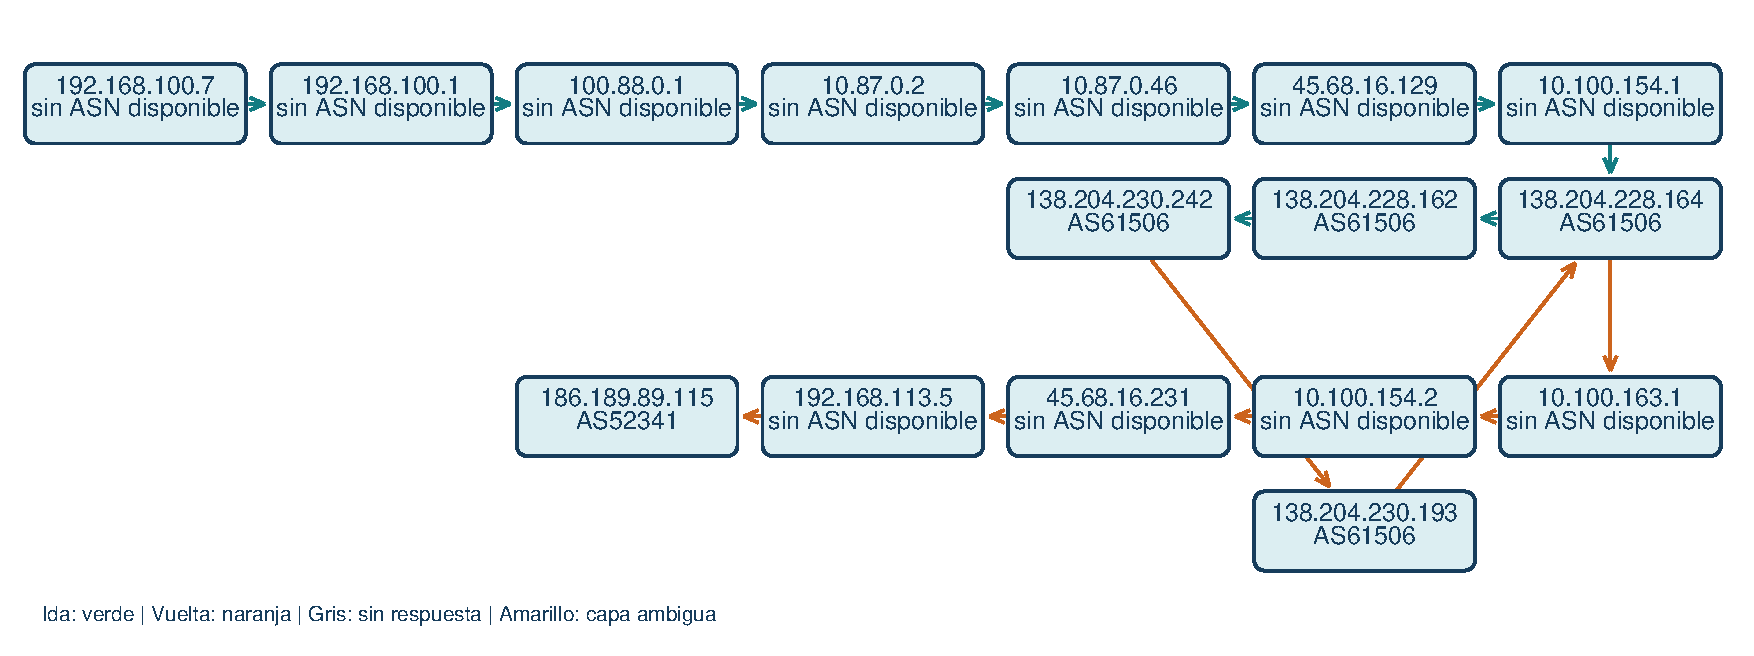
\includegraphics[width=\linewidth,height=.62\textheight,keepaspectratio]{figuras/grafo_138.204.230.242.pdf}
\captionof{figure}{Representación vectorial del mismo CX2 publicado, Valparaíso. Las flechas indican sentido; las aristas son inferidas. Las capturas reales de NDEx se incluyen en el anexo.}\label{grafo:138.204.230.242}
\end{landscape}
\begin{landscape}
\subsubsection{La Habana}
Par elegido: TCP, ronda 2. Unión de 26 IP; 9 TTL sin respuesta en conjunto. Ida 227953132; vuelta 227953345.

UUID: fa23a62a-d1b2-11f1-be0a-005056ae3c32

\noindent\url{https://www.ndexbio.org/viewer/networks/fa23a62a-d1b2-11f1-be0a-005056ae3c32}\par\medskip
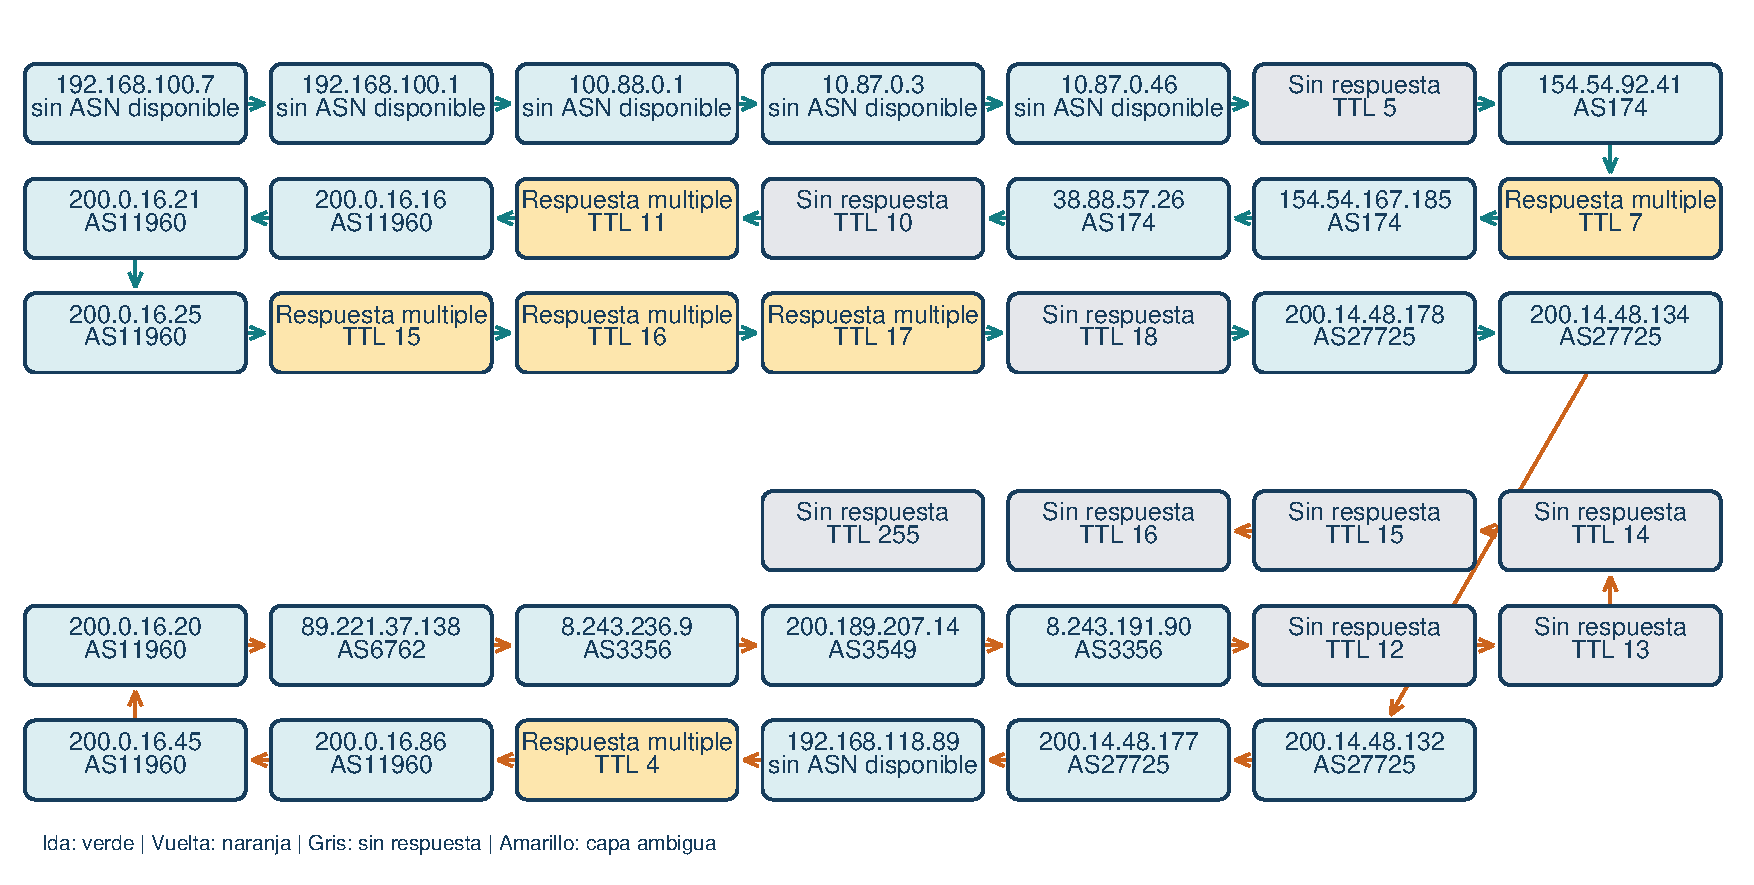
\includegraphics[width=\linewidth,height=.62\textheight,keepaspectratio]{figuras/grafo_200.14.48.134.pdf}
\captionof{figure}{Representación vectorial del mismo CX2 publicado, La Habana. Las flechas indican sentido; las aristas son inferidas. Las capturas reales de NDEx se incluyen en el anexo.}\label{grafo:200.14.48.134}
\end{landscape}
\begin{landscape}
\subsubsection{Rusia}
Par elegido: ICMP, ronda 3. Unión de 20 IP; 4 TTL sin respuesta en conjunto. Ida 228276628; vuelta 228277013.

UUID: 6f78f82e-d219-11f1-be0a-005056ae3c32

\noindent\url{https://www.ndexbio.org/viewer/networks/6f78f82e-d219-11f1-be0a-005056ae3c32}\par\medskip
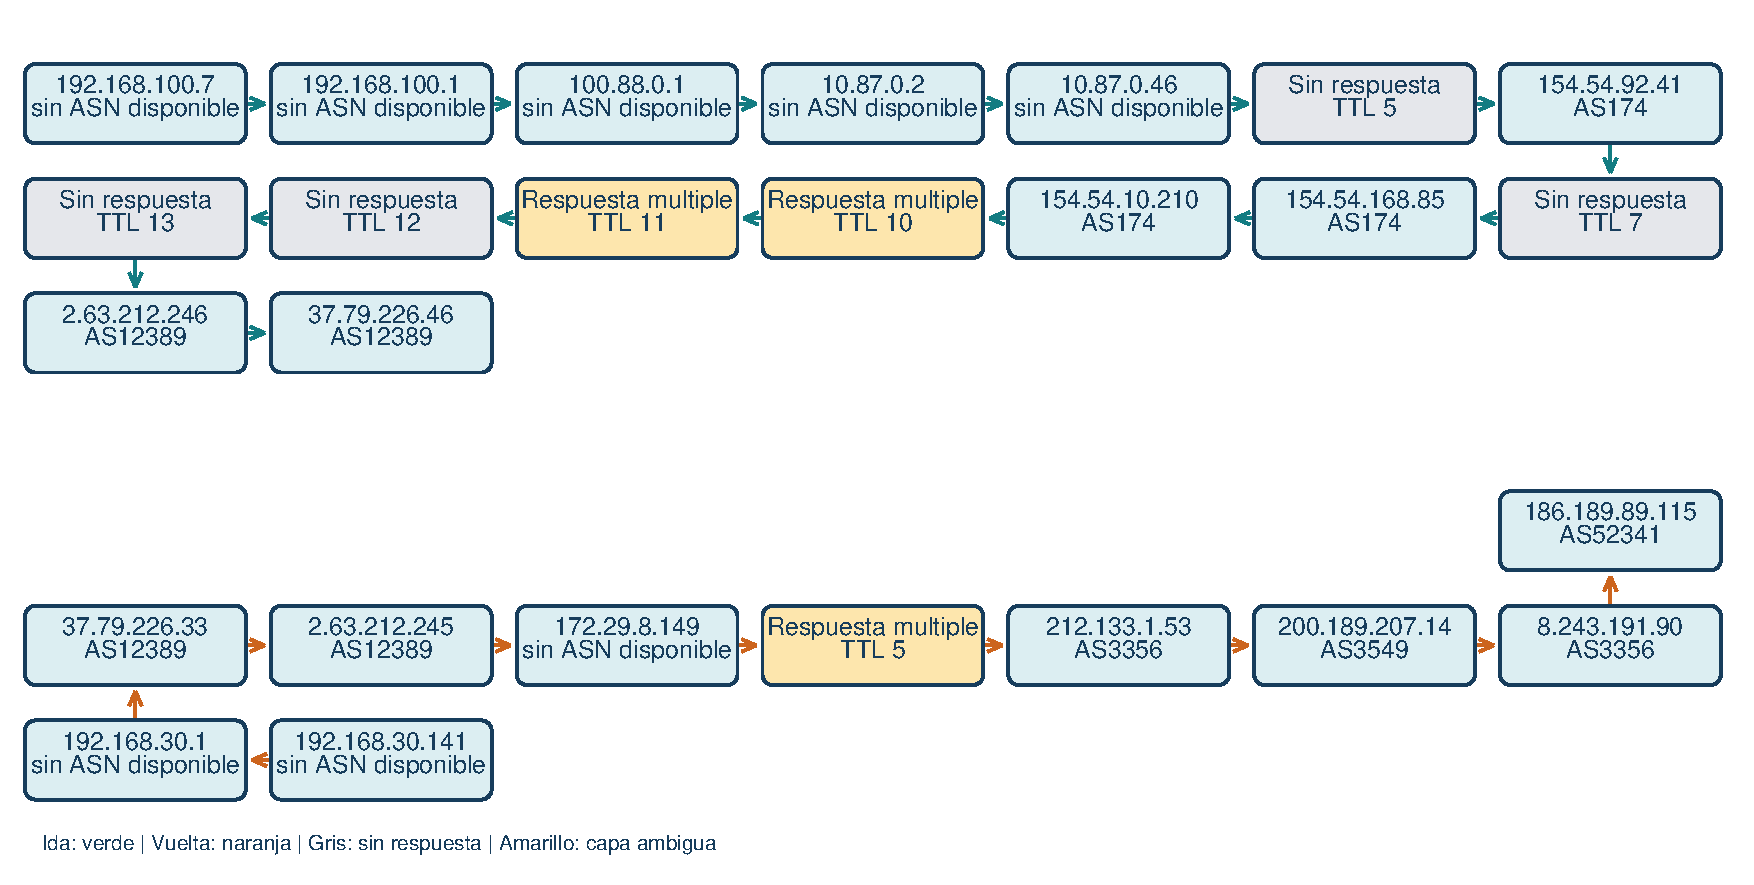
\includegraphics[width=\linewidth,height=.62\textheight,keepaspectratio]{figuras/grafo_37.79.226.46.pdf}
\captionof{figure}{Representación vectorial del mismo CX2 publicado, Rusia. Las flechas indican sentido; las aristas son inferidas. Las capturas reales de NDEx se incluyen en el anexo.}\label{grafo:37.79.226.46}
\end{landscape}


\clearpage
\section{Conclusión}\label{sec:conclusion}
Las tres rondas muestran que el método más informativo depende del destino y del criterio aplicado. La comparación se apoya en medianas de IP únicas, cobertura y estabilidad, y conserva el costo de exploración.

Valparaíso: scamper: icmp, icmp-paris, udp, udp-paris (mediana 9 IP); ripe: ICMP, TCP, UDP (mediana 9 IP).

La Habana: scamper: icmp, icmp-paris (mediana 13 IP); ripe: TCP (mediana 14 IP).

Rusia: scamper: icmp, icmp-paris (mediana 12 IP); ripe: TCP (mediana 11 IP).

tracelb permite revelar interfaces adicionales en algunos modos y destinos, con distinto costo en sondas. Las diferencias entre Chile, Cuba y Rusia describen las rutas y horarios medidos; no deben interpretarse como una clasificación de velocidades o de censura.

Ida y vuelta no ofrecieron evidencia suficiente para afirmar simetría completa en las rutas incompletas. Las observaciones corresponden a interfaces; la identificación de routers físicos requiere corroboración adicional de alias. La respuesta selectiva sí se repitió en los casos documentados, pero no identifica por sí sola una regla de filtrado.

El aprendizaje principal es que la calidad de Path Discovery depende tanto del método como de la captura, la recepción local y la trazabilidad. Para repetir el estudio conviene preservar originales, contrastar parámetros efectivos, verificar la continuidad de la sesión y comparar pares próximos temporalmente. El diagnóstico TCP demuestra por qué una ausencia en la salida de una herramienta debe contrastarse con los paquetes antes de atribuirla a la red.



\clearpage
\section{Anexos}\label{sec:anexos}
\subsection{Imágenes de Wireshark y NDEx}\label{anexo:imagenes}
Las siguientes capturas corresponden a la interfaz gráfica real. Cada una está vinculada a un original y a su hash en el inventario digital. Son evidencia complementaria; los valores legibles y las reglas se desarrollan en el cuerpo principal.

\begin{landscape}
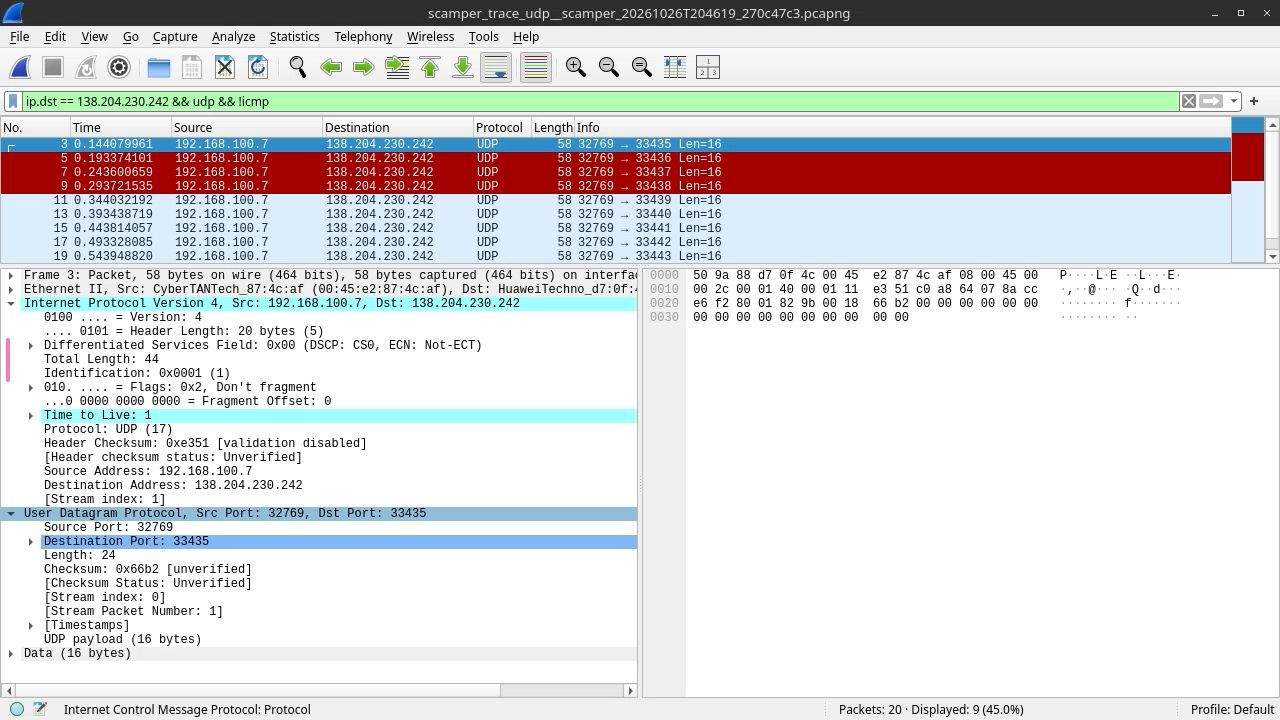
\includegraphics[width=\linewidth,height=.83\textheight,keepaspectratio]{figuras/wireshark_scamper_trace_udp_casa204144.jpg}
\captionof{figure}{Wireshark: scamper\_\allowbreak{}trace\_\allowbreak{}udp. Original scamper\_\allowbreak{}20261026T204619\_\allowbreak{}270c47c3. Encabezados y bytes observados; el contraste temporal se realiza con las rondas posteriores.}
\end{landscape}
\begin{landscape}
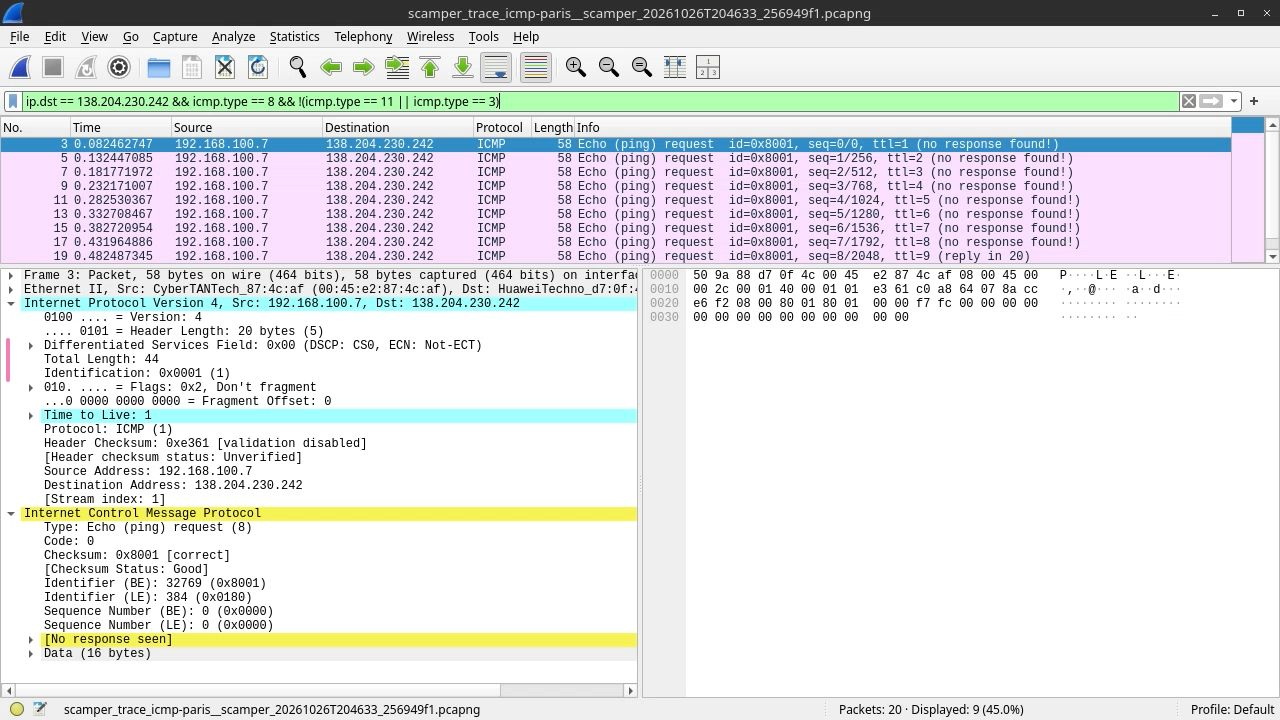
\includegraphics[width=\linewidth,height=.83\textheight,keepaspectratio]{figuras/wireshark_scamper_trace_icmp-paris_casa204144.jpg}
\captionof{figure}{Wireshark: scamper\_\allowbreak{}trace\_\allowbreak{}icmp-paris. Original scamper\_\allowbreak{}20261026T204633\_\allowbreak{}256949f1. Encabezados y bytes observados; el contraste temporal se realiza con las rondas posteriores.}
\end{landscape}
\begin{landscape}
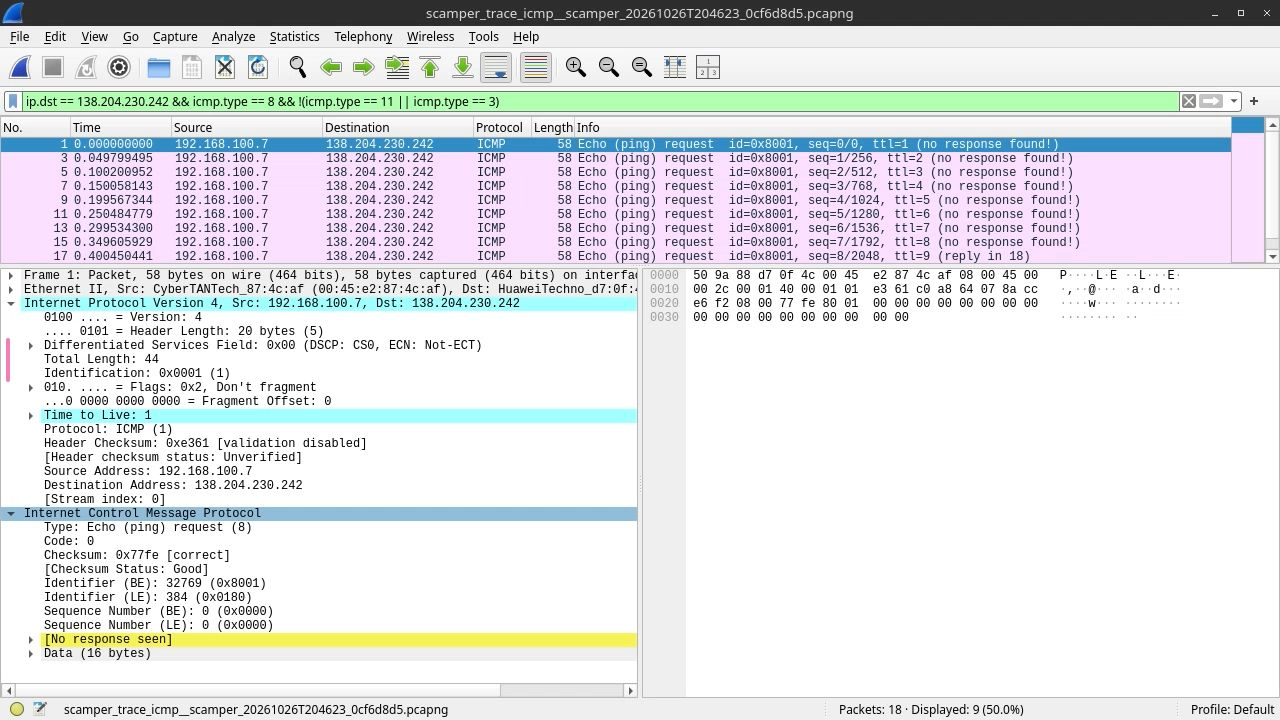
\includegraphics[width=\linewidth,height=.83\textheight,keepaspectratio]{figuras/wireshark_scamper_trace_icmp_casa204144.jpg}
\captionof{figure}{Wireshark: scamper\_\allowbreak{}trace\_\allowbreak{}icmp. Original scamper\_\allowbreak{}20261026T204623\_\allowbreak{}0cf6d8d5. Encabezados y bytes observados; el contraste temporal se realiza con las rondas posteriores.}
\end{landscape}
\begin{landscape}
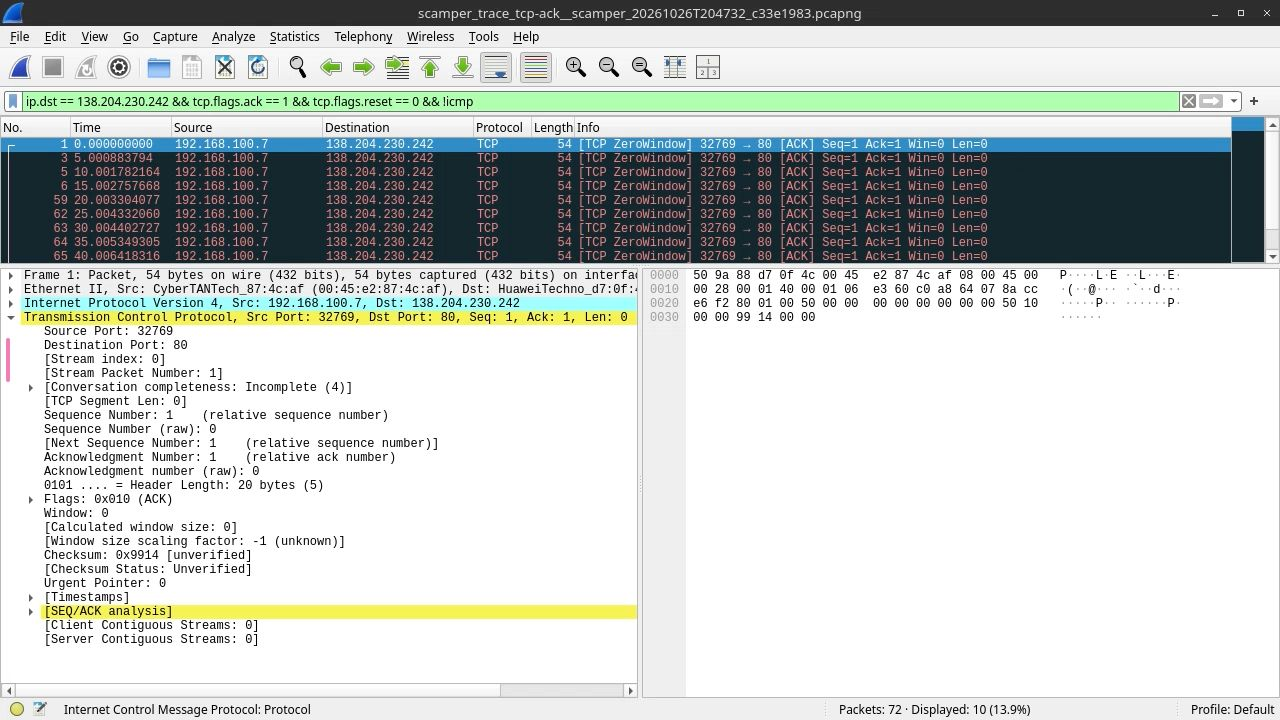
\includegraphics[width=\linewidth,height=.83\textheight,keepaspectratio]{figuras/wireshark_scamper_trace_tcp-ack_casa204144.jpg}
\captionof{figure}{Wireshark: scamper\_\allowbreak{}trace\_\allowbreak{}tcp-ack. Original scamper\_\allowbreak{}20261026T204732\_\allowbreak{}c33e1983. Encabezados y bytes observados; el contraste temporal se realiza con las rondas posteriores.}
\end{landscape}
\begin{landscape}
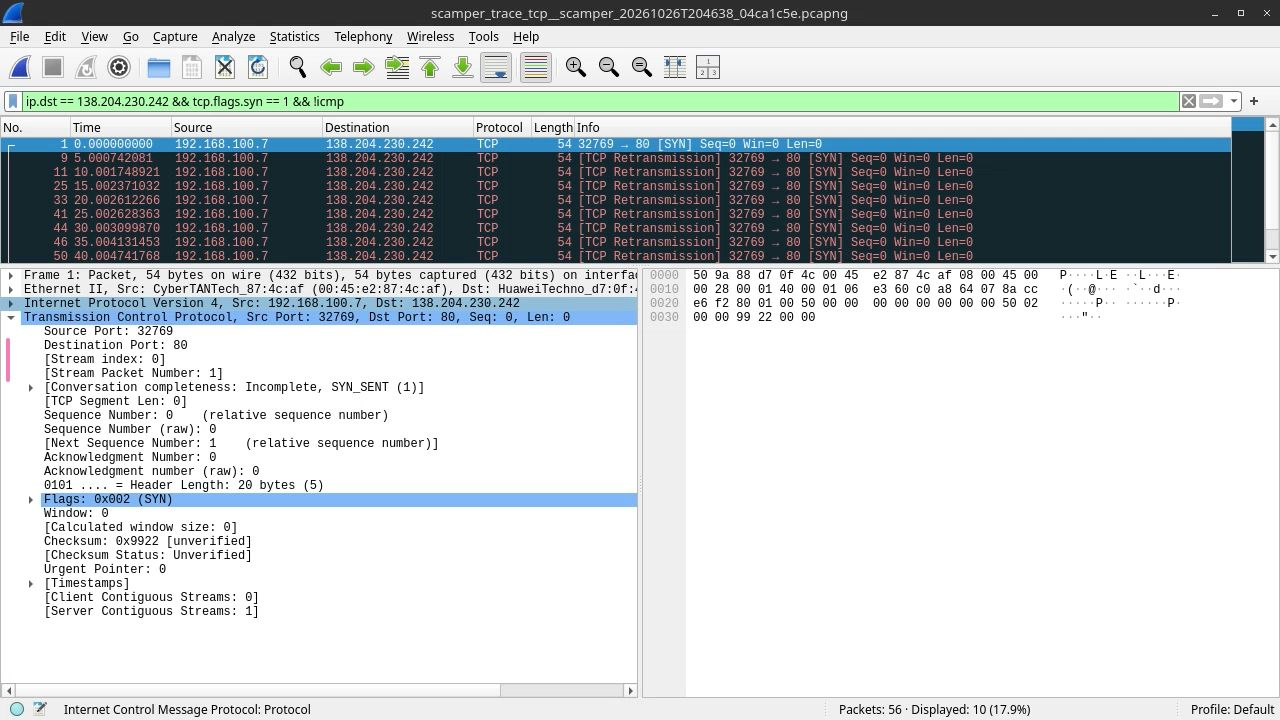
\includegraphics[width=\linewidth,height=.83\textheight,keepaspectratio]{figuras/wireshark_scamper_trace_tcp_casa204144.jpg}
\captionof{figure}{Wireshark: scamper\_\allowbreak{}trace\_\allowbreak{}tcp. Original scamper\_\allowbreak{}20261026T204638\_\allowbreak{}04ca1c5e. Encabezados y bytes observados; el contraste temporal se realiza con las rondas posteriores.}
\end{landscape}
\begin{landscape}
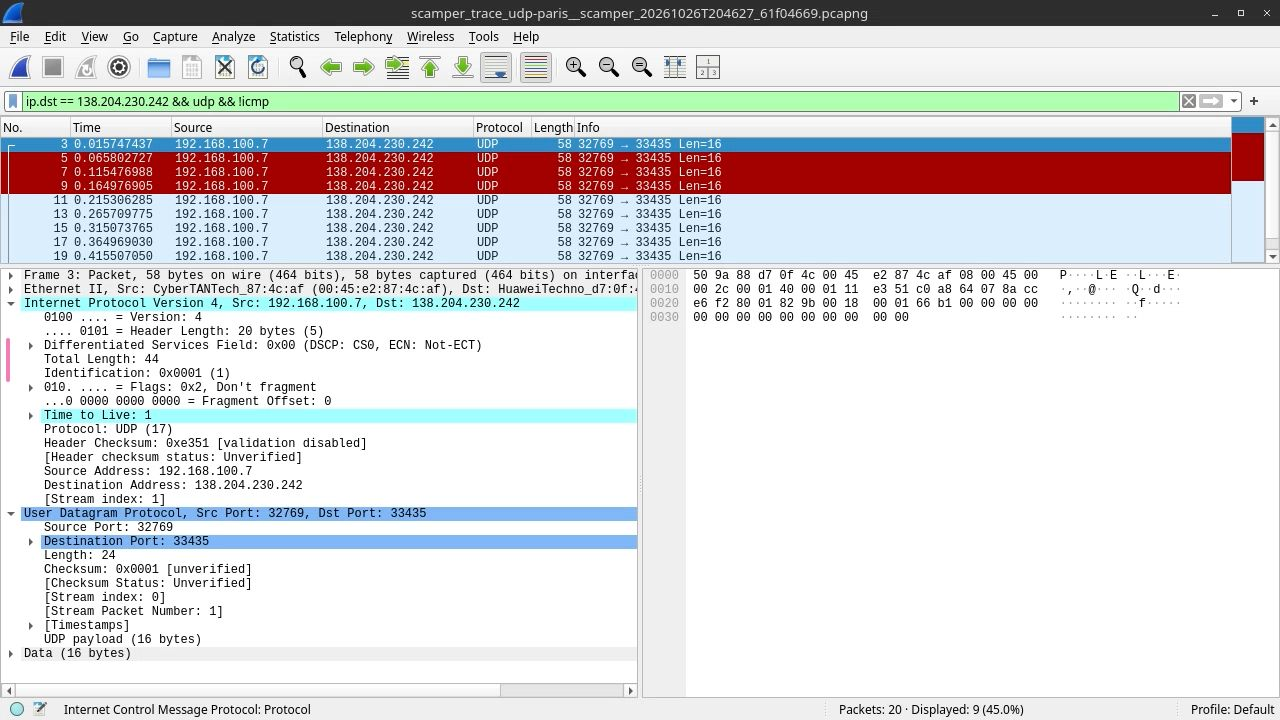
\includegraphics[width=\linewidth,height=.83\textheight,keepaspectratio]{figuras/wireshark_scamper_trace_udp-paris_casa204144.jpg}
\captionof{figure}{Wireshark: scamper\_\allowbreak{}trace\_\allowbreak{}udp-paris. Original scamper\_\allowbreak{}20261026T204627\_\allowbreak{}61f04669. Encabezados y bytes observados; el contraste temporal se realiza con las rondas posteriores.}
\end{landscape}
\begin{landscape}
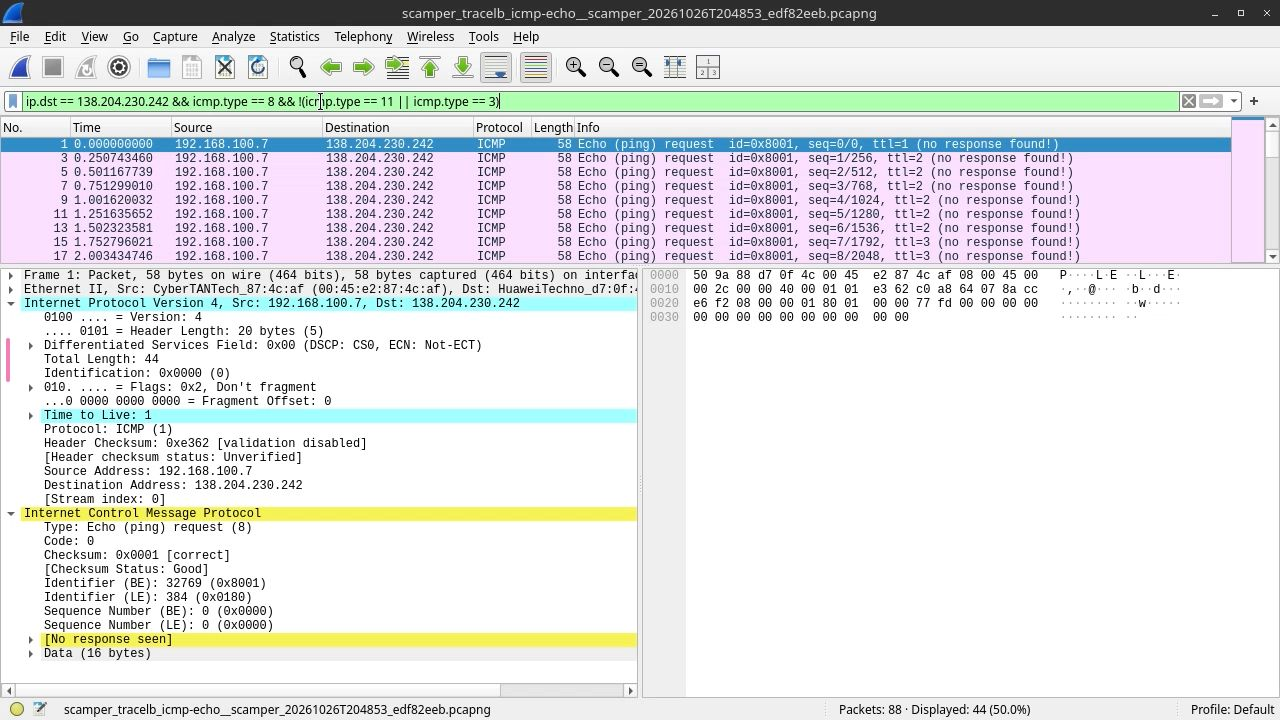
\includegraphics[width=\linewidth,height=.83\textheight,keepaspectratio]{figuras/wireshark_scamper_tracelb_icmp-echo_casa204144.jpg}
\captionof{figure}{Wireshark: scamper\_\allowbreak{}tracelb\_\allowbreak{}icmp-echo. Original scamper\_\allowbreak{}20261026T204853\_\allowbreak{}edf82eeb. Encabezados y bytes observados; el contraste temporal se realiza con las rondas posteriores.}
\end{landscape}
\begin{landscape}
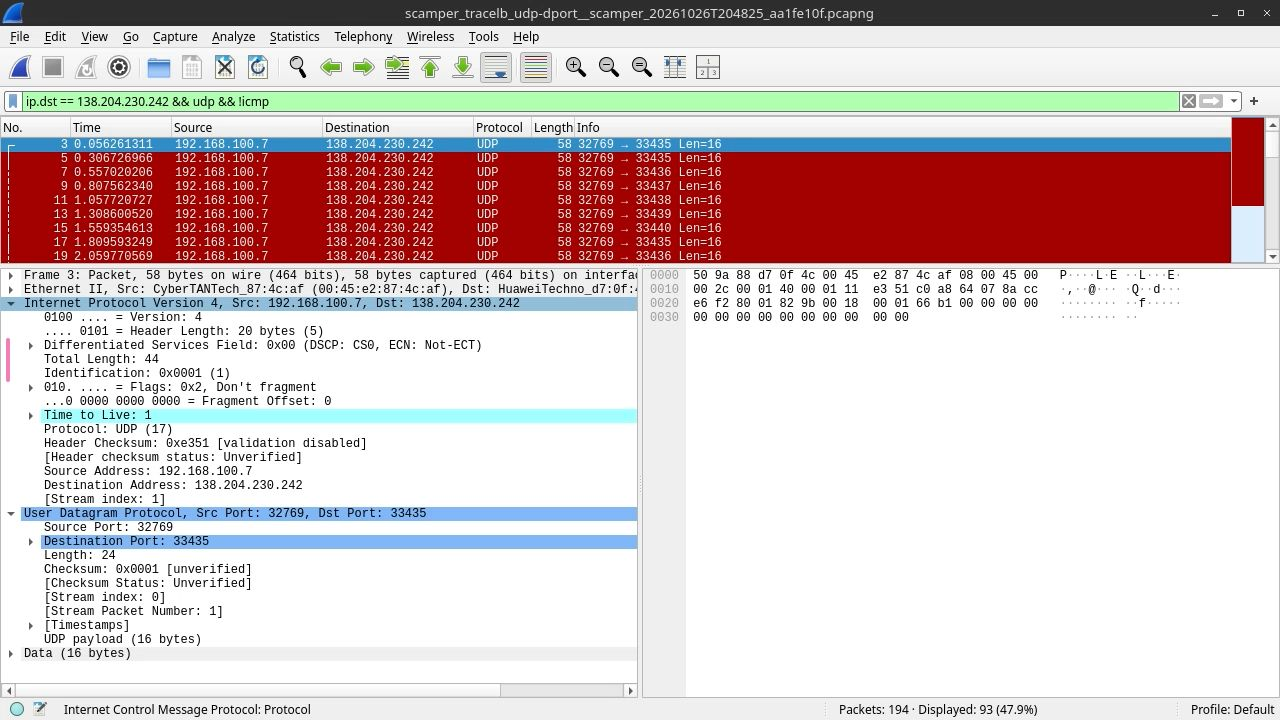
\includegraphics[width=\linewidth,height=.83\textheight,keepaspectratio]{figuras/wireshark_scamper_tracelb_udp-dport_casa204144.jpg}
\captionof{figure}{Wireshark: scamper\_\allowbreak{}tracelb\_\allowbreak{}udp-dport. Original scamper\_\allowbreak{}20261026T204825\_\allowbreak{}aa1fe10f. Encabezados y bytes observados; el contraste temporal se realiza con las rondas posteriores.}
\end{landscape}
\begin{landscape}
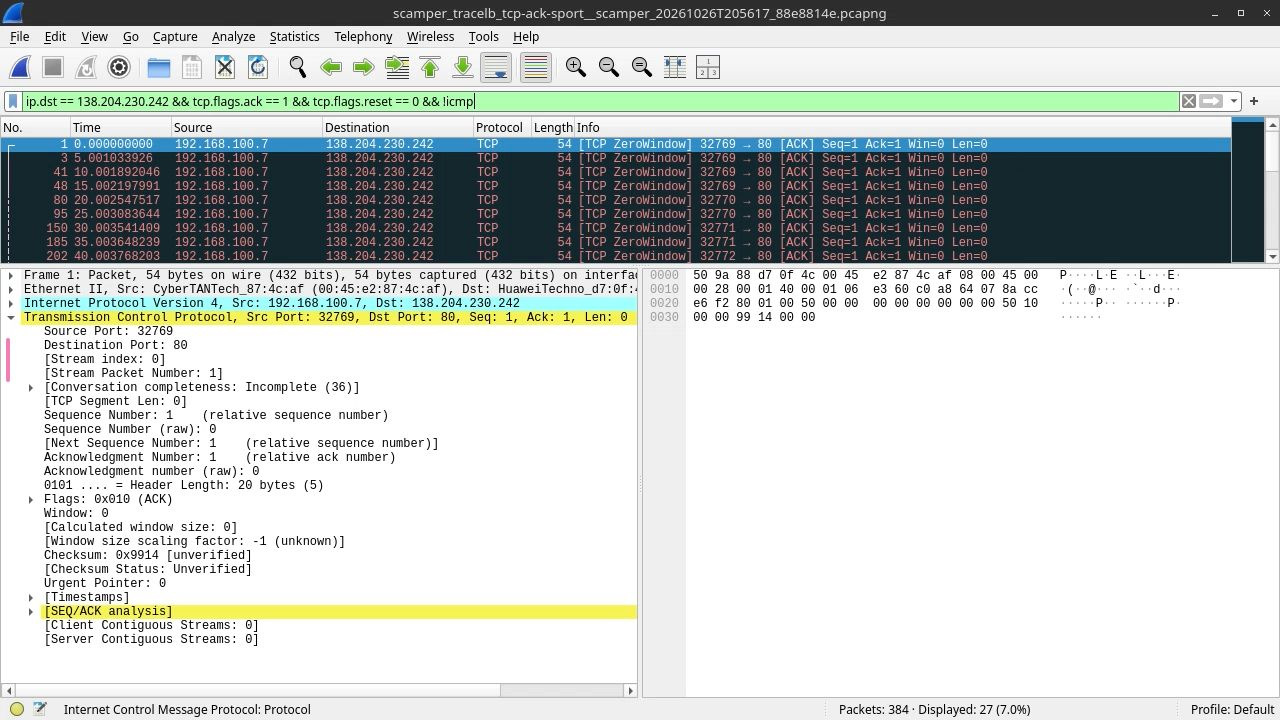
\includegraphics[width=\linewidth,height=.83\textheight,keepaspectratio]{figuras/wireshark_scamper_tracelb_tcp-ack-sport_casa204144.jpg}
\captionof{figure}{Wireshark: scamper\_\allowbreak{}tracelb\_\allowbreak{}tcp-ack-sport. Original scamper\_\allowbreak{}20261026T205617\_\allowbreak{}88e8814e. Encabezados y bytes observados; el contraste temporal se realiza con las rondas posteriores.}
\end{landscape}
\begin{landscape}
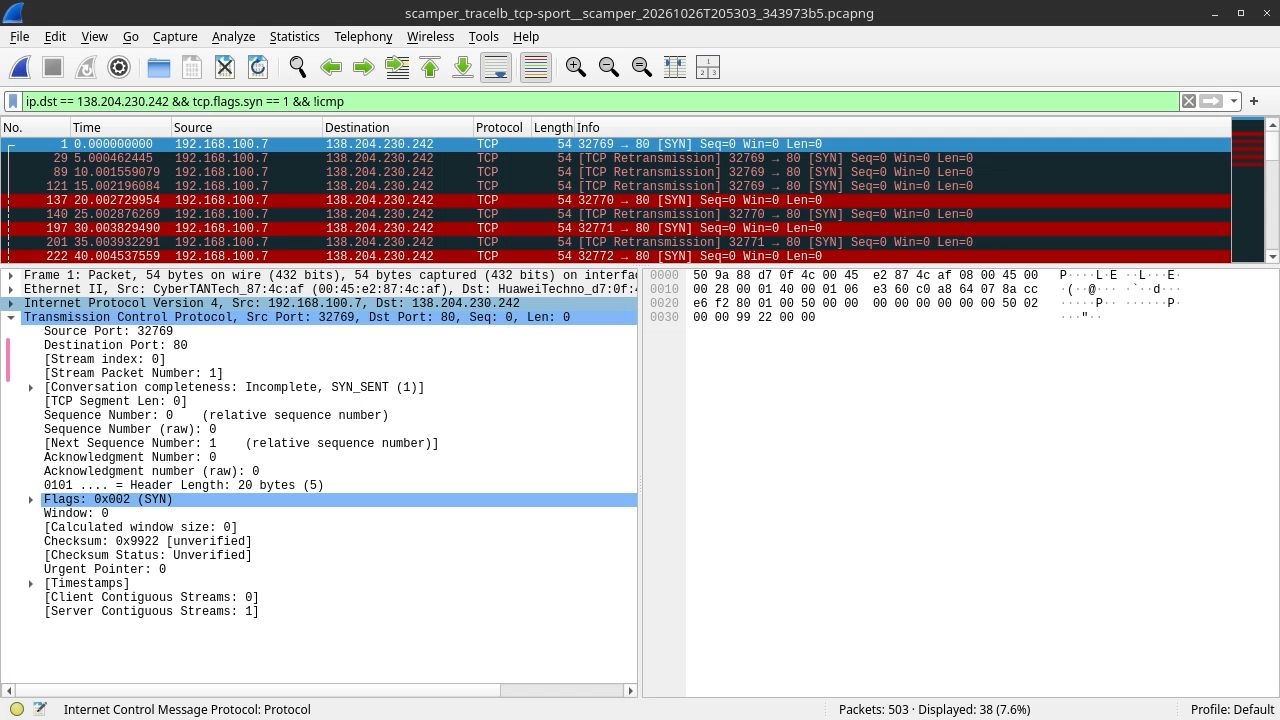
\includegraphics[width=\linewidth,height=.83\textheight,keepaspectratio]{figuras/wireshark_scamper_tracelb_tcp-sport_casa204144.jpg}
\captionof{figure}{Wireshark: scamper\_\allowbreak{}tracelb\_\allowbreak{}tcp-sport. Original scamper\_\allowbreak{}20261026T205303\_\allowbreak{}343973b5. Encabezados y bytes observados; el contraste temporal se realiza con las rondas posteriores.}
\end{landscape}
\begin{landscape}
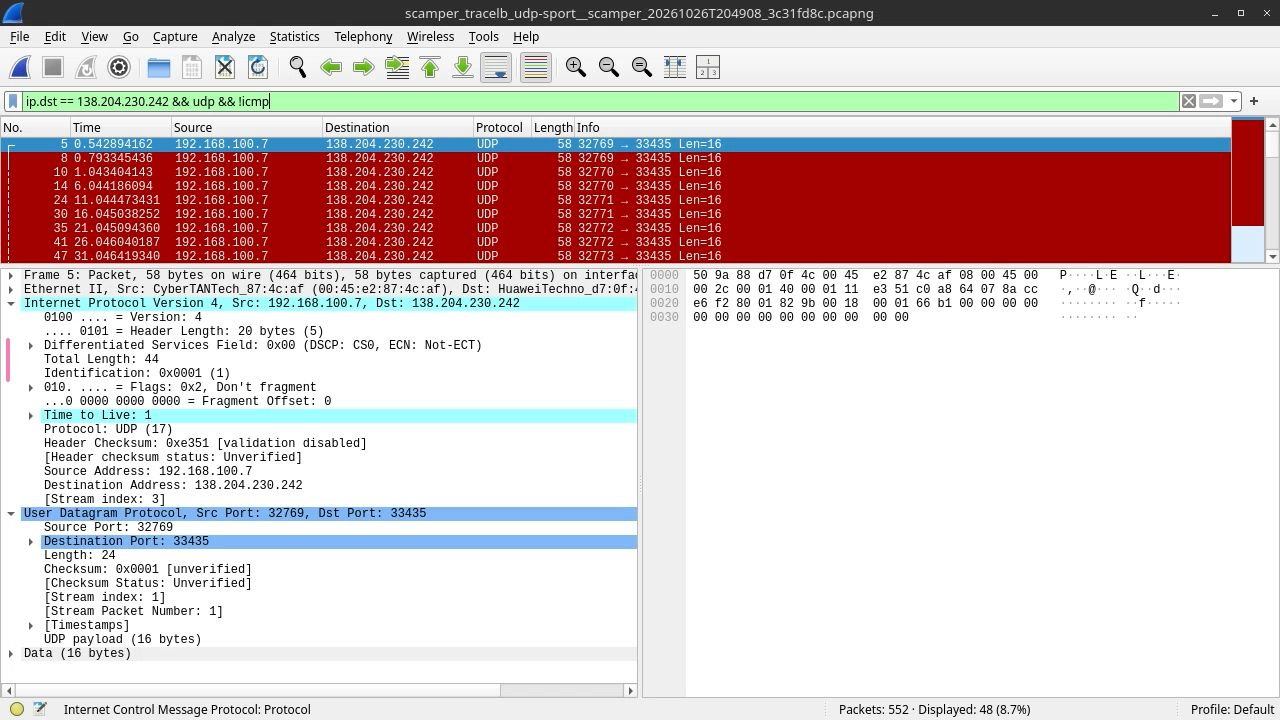
\includegraphics[width=\linewidth,height=.83\textheight,keepaspectratio]{figuras/wireshark_scamper_tracelb_udp-sport_casa204144.jpg}
\captionof{figure}{Wireshark: scamper\_\allowbreak{}tracelb\_\allowbreak{}udp-sport. Original scamper\_\allowbreak{}20261026T204908\_\allowbreak{}3c31fd8c. Encabezados y bytes observados; el contraste temporal se realiza con las rondas posteriores.}
\end{landscape}
\begin{landscape}
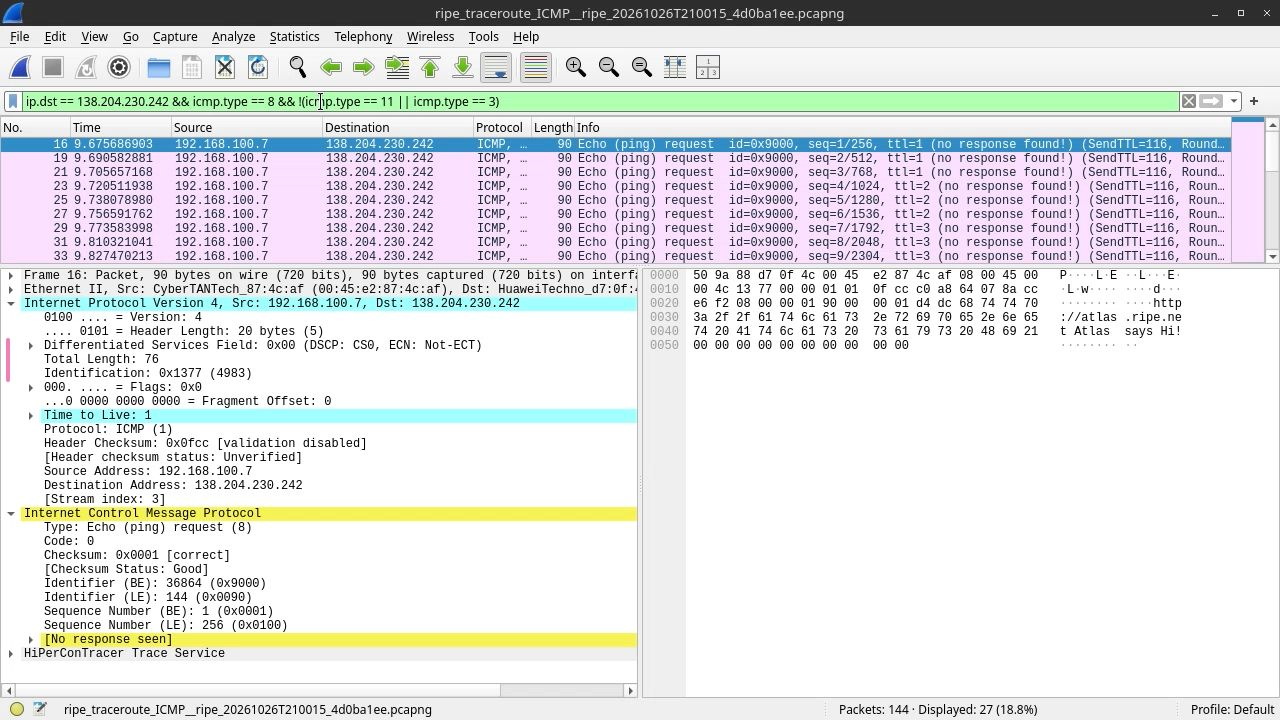
\includegraphics[width=\linewidth,height=.83\textheight,keepaspectratio]{figuras/wireshark_ripe_traceroute_ICMP_casa204144.jpg}
\captionof{figure}{Wireshark: ripe\_\allowbreak{}traceroute\_\allowbreak{}ICMP. Original ripe\_\allowbreak{}20261026T210015\_\allowbreak{}4d0ba1ee. Encabezados y bytes observados; el contraste temporal se realiza con las rondas posteriores.}
\end{landscape}
\begin{landscape}
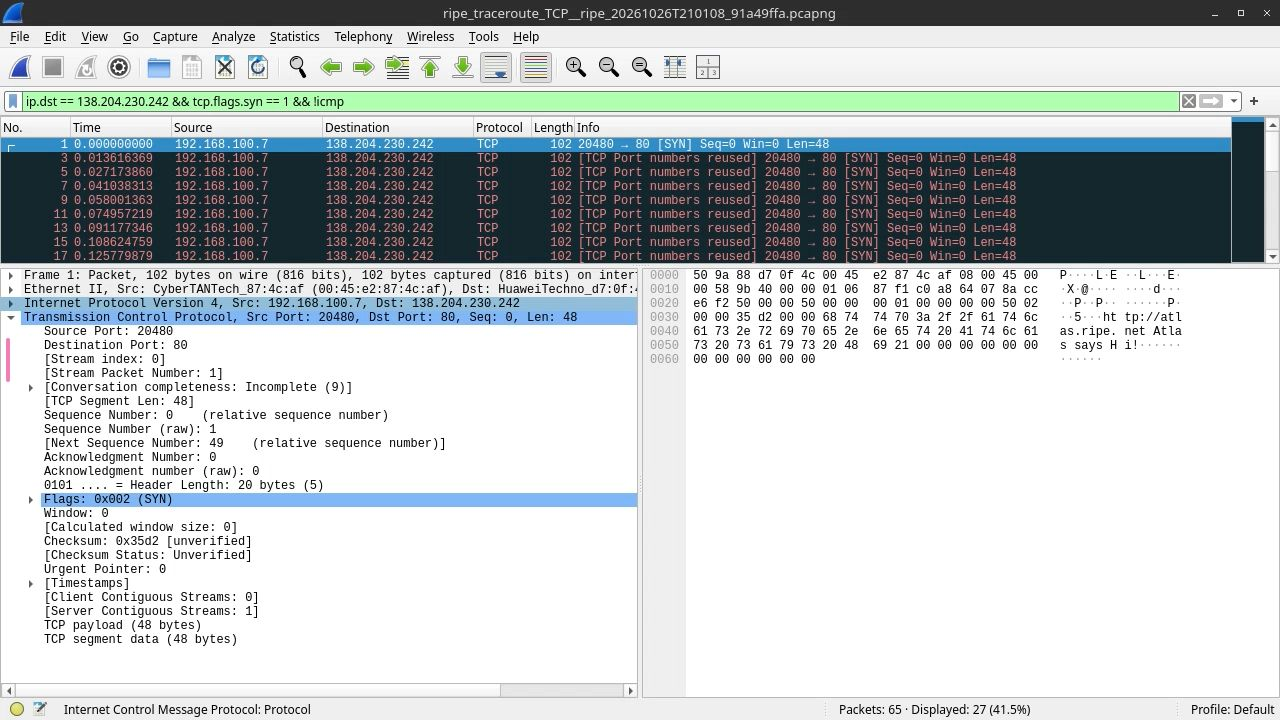
\includegraphics[width=\linewidth,height=.83\textheight,keepaspectratio]{figuras/wireshark_ripe_traceroute_TCP_casa204144.jpg}
\captionof{figure}{Wireshark: ripe\_\allowbreak{}traceroute\_\allowbreak{}TCP. Original ripe\_\allowbreak{}20261026T210108\_\allowbreak{}91a49ffa. Encabezados y bytes observados; el contraste temporal se realiza con las rondas posteriores.}
\end{landscape}
\begin{landscape}
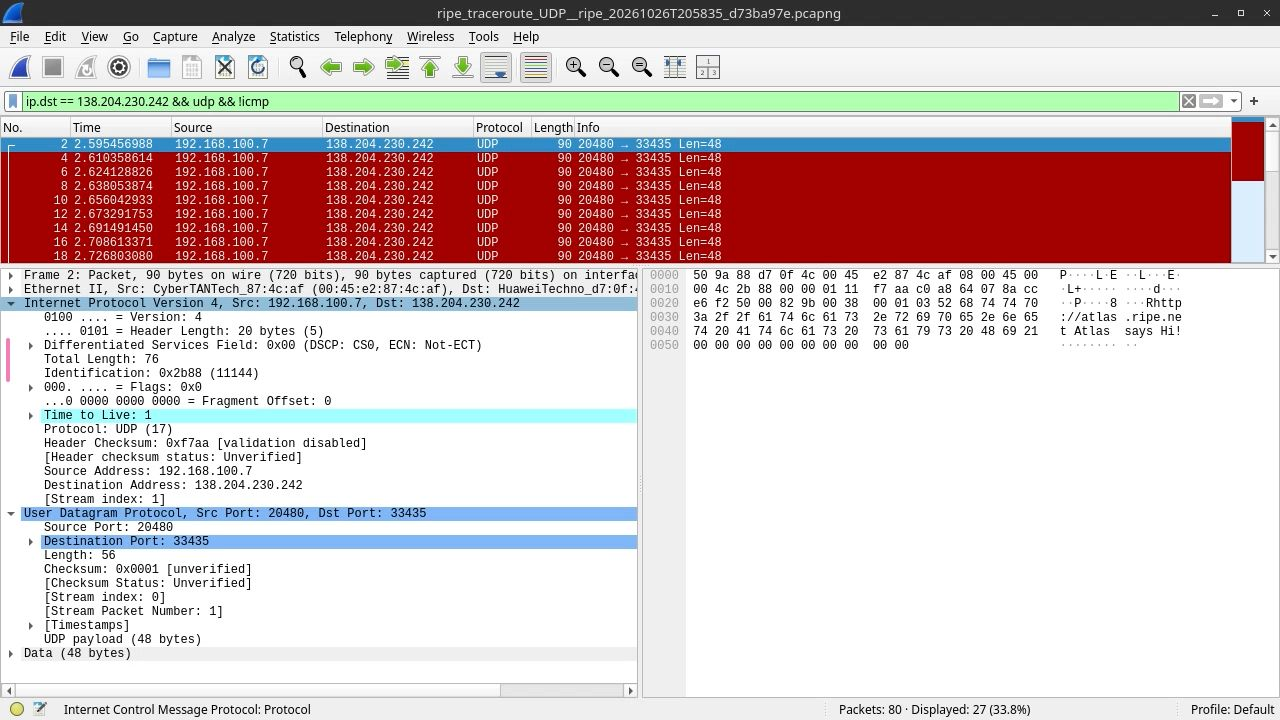
\includegraphics[width=\linewidth,height=.83\textheight,keepaspectratio]{figuras/wireshark_ripe_traceroute_UDP_casa204144.jpg}
\captionof{figure}{Wireshark: ripe\_\allowbreak{}traceroute\_\allowbreak{}UDP. Original ripe\_\allowbreak{}20261026T205835\_\allowbreak{}d73ba97e. Encabezados y bytes observados; el contraste temporal se realiza con las rondas posteriores.}
\end{landscape}
\begin{landscape}
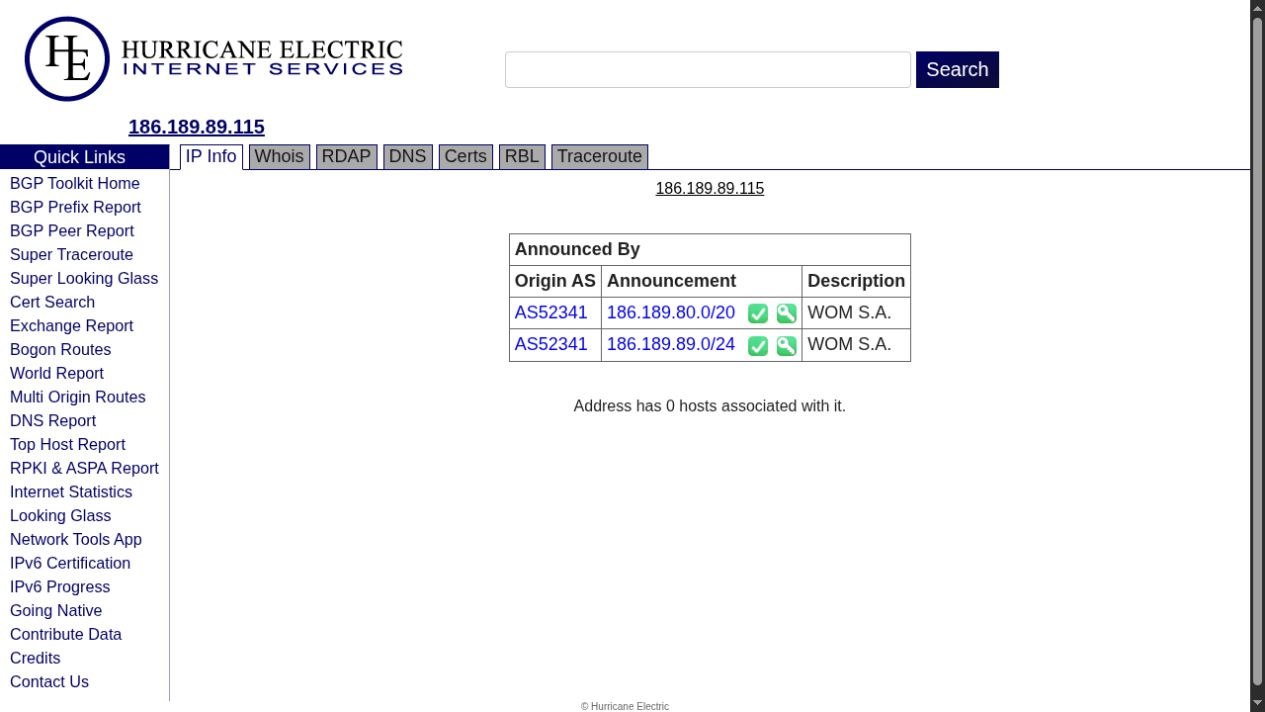
\includegraphics[width=\linewidth,height=.82\textheight,keepaspectratio]{figuras/bgp_he_origen.jpg}
\captionof{figure}{BGP HE: IPv4 186.189.89.115, AS52341 (WOM S.A.), anuncios 186.189.80.0/20 y 186.189.89.0/24; consulta del 27 de octubre de 2026.}
\end{landscape}
\begin{landscape}
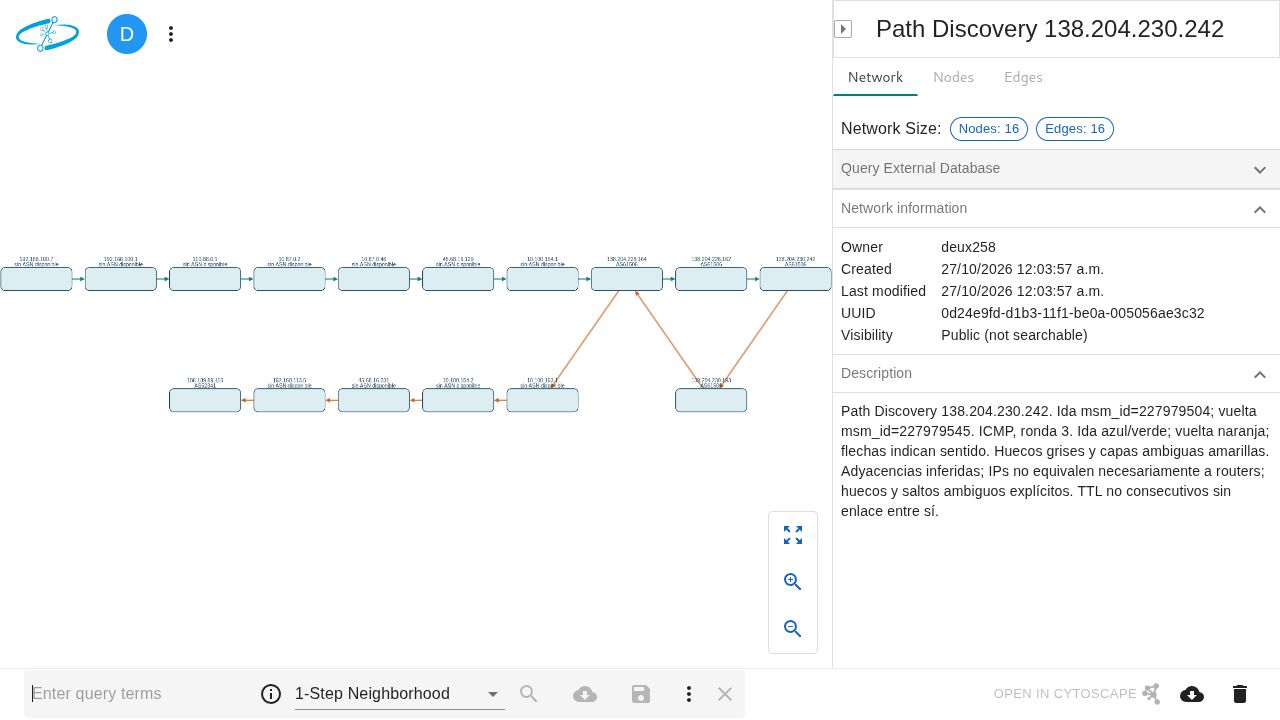
\includegraphics[width=\linewidth,height=.82\textheight,keepaspectratio]{figuras/ndex_valparaiso_publico.jpg}
\captionof{figure}{Grafo definitivo de Valparaíso en NDEx. Visibilidad Public, UUID 0d24e9fd-d1b3-11f1-be0a-005056ae3c32. La ficha conserva los dos IDs RIPE.}
\end{landscape}
\begin{landscape}
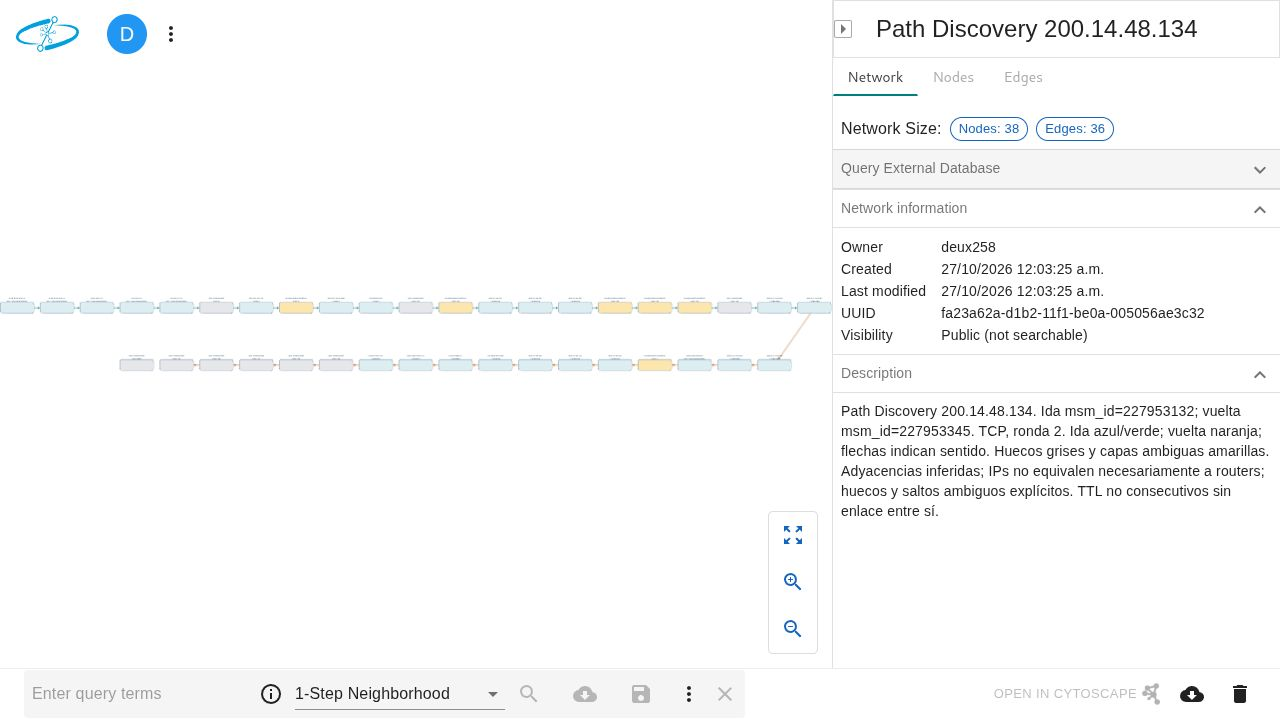
\includegraphics[width=\linewidth,height=.82\textheight,keepaspectratio]{figuras/ndex_habana_publico.jpg}
\captionof{figure}{Grafo definitivo de La Habana en NDEx. Visibilidad Public, UUID fa23a62a-d1b2-11f1-be0a-005056ae3c32. La ficha conserva los dos IDs RIPE.}
\end{landscape}
\begin{landscape}
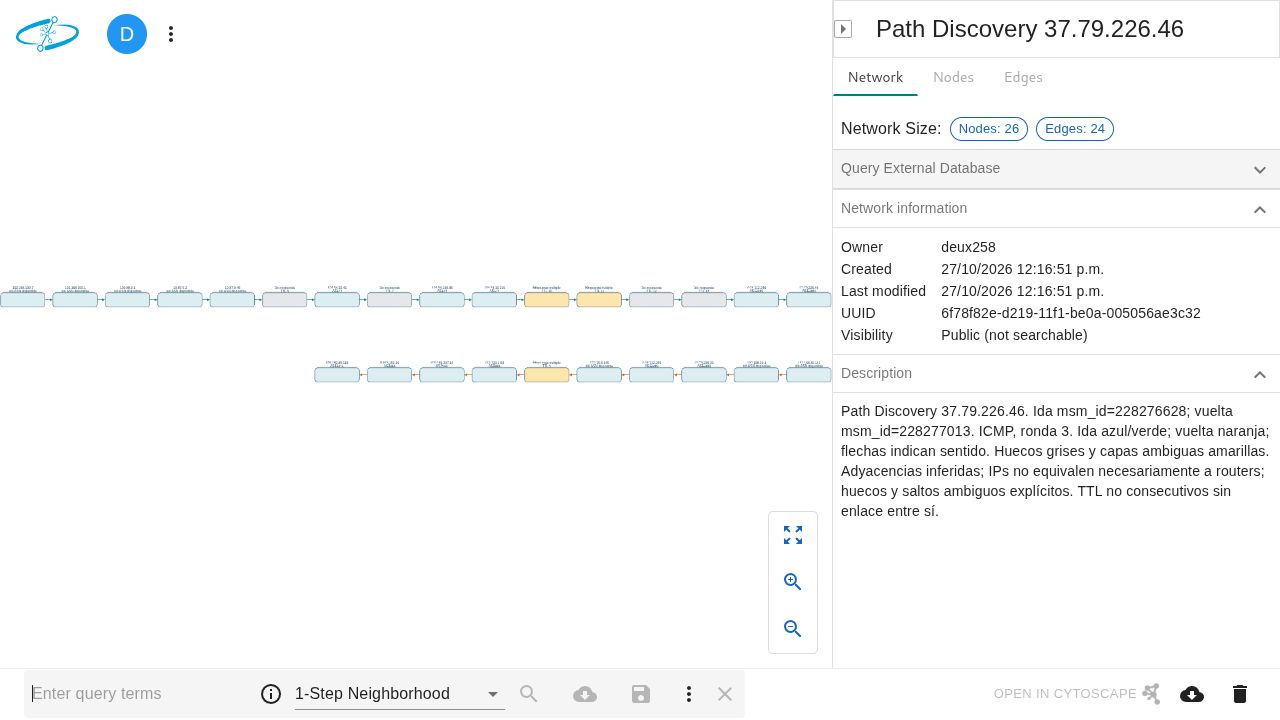
\includegraphics[width=\linewidth,height=.82\textheight,keepaspectratio]{figuras/ndex_rusia_publico.jpg}
\captionof{figure}{Grafo definitivo de Rusia en NDEx: visibilidad Public, UUID 6f78f82e-d219-11f1-be0a-005056ae3c32, mediciones 228276628 y 228277013; 26 nodos y 24 aristas.}
\end{landscape}
\begin{landscape}
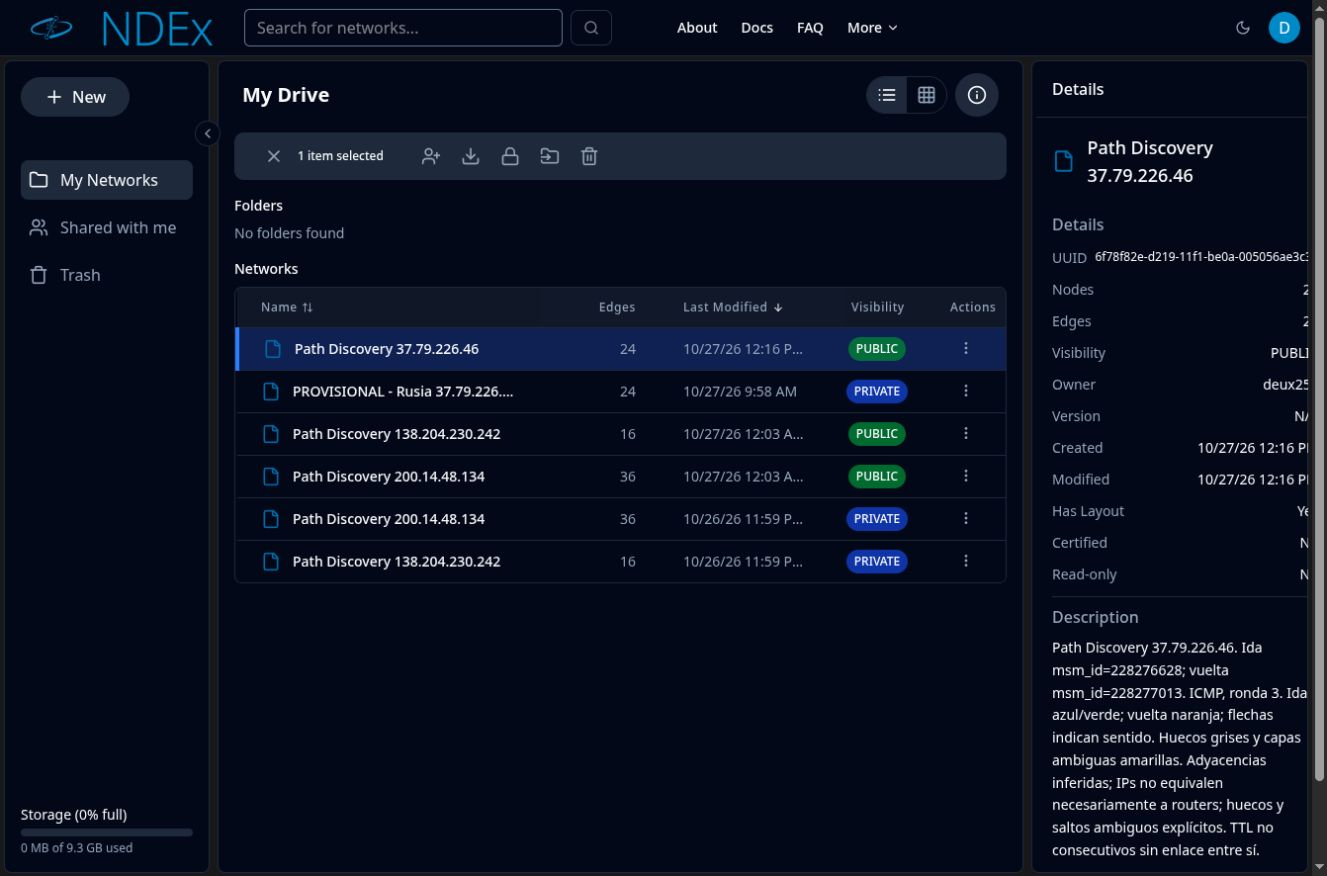
\includegraphics[width=\linewidth,height=.82\textheight,keepaspectratio]{figuras/ndex_tres_grafos_publicos.jpg}
\captionof{figure}{NDEx: tres grafos definitivos con visibilidad PUBLIC, verificados mediante acceso anónimo.}
\end{landscape}
\subsection{Comandos completos, tablas y originales}\label{anexo:originales}
Los WARTS, JSON y PCAPNG se entregan como archivos digitales para conservar la evidencia completa sin imprimir miles de registros. El manifiesto de fuentes enlaza cada tabla y figura con su archivo, versión y hash. Se conserva una respuesta por intento y TTL; las tablas siguientes compactan las respuestas múltiples por celda.

\subsubsection{Comandos efectivos por método}
\paragraph{ripe / traceroute / UDP / ida}
\begin{lstlisting}
{
  "definitions": [
    {
      "target": "138.204.230.242",
      "description": "PathDiscovery Valparaiso ida UDP",
      "type": "traceroute",
      "af": 4,
      "protocol": "UDP"
    }
  ],
  "probes": [
    {
      "requested": 1,
      "type": "probes",
      "value": "1018487"
    }
  ],
  "is_oneoff": true
}
\end{lstlisting}
\paragraph{ripe / traceroute / UDP / vuelta}
\begin{lstlisting}
{
  "definitions": [
    {
      "target": "186.189.89.115",
      "description": "PathDiscovery Valparaiso vuelta UDP",
      "type": "traceroute",
      "af": 4,
      "protocol": "UDP"
    }
  ],
  "probes": [
    {
      "requested": 1,
      "type": "probes",
      "value": "6652"
    }
  ],
  "is_oneoff": true
}
\end{lstlisting}
\paragraph{ripe / traceroute / ICMP / ida}
\begin{lstlisting}
{
  "definitions": [
    {
      "target": "138.204.230.242",
      "description": "PathDiscovery Valparaiso ida ICMP",
      "type": "traceroute",
      "af": 4,
      "protocol": "ICMP"
    }
  ],
  "probes": [
    {
      "requested": 1,
      "type": "probes",
      "value": "1018487"
    }
  ],
  "is_oneoff": true
}
\end{lstlisting}
\paragraph{ripe / traceroute / ICMP / vuelta}
\begin{lstlisting}
{
  "definitions": [
    {
      "target": "186.189.89.115",
      "description": "PathDiscovery Valparaiso vuelta ICMP",
      "type": "traceroute",
      "af": 4,
      "protocol": "ICMP"
    }
  ],
  "probes": [
    {
      "requested": 1,
      "type": "probes",
      "value": "6652"
    }
  ],
  "is_oneoff": true
}
\end{lstlisting}
\paragraph{ripe / traceroute / TCP / ida}
\begin{lstlisting}
{
  "definitions": [
    {
      "target": "138.204.230.242",
      "description": "PathDiscovery Valparaiso ida TCP",
      "type": "traceroute",
      "af": 4,
      "protocol": "TCP",
      "port": 80
    }
  ],
  "probes": [
    {
      "requested": 1,
      "type": "probes",
      "value": "1018487"
    }
  ],
  "is_oneoff": true
}
\end{lstlisting}
\paragraph{ripe / traceroute / TCP / vuelta}
\begin{lstlisting}
{
  "definitions": [
    {
      "target": "186.189.89.115",
      "description": "PathDiscovery Valparaiso vuelta TCP",
      "type": "traceroute",
      "af": 4,
      "protocol": "TCP",
      "port": 80
    }
  ],
  "probes": [
    {
      "requested": 1,
      "type": "probes",
      "value": "6652"
    }
  ],
  "is_oneoff": true
}
\end{lstlisting}
\paragraph{scamper / trace / udp / ida}
\begin{lstlisting}
env PD_TOOL_IMAGE=path-discovery-tools:20260902 docker compose --env-file /dev/null --project-directory /home/diego/Documentos/GitHub/Alg_Ruteo_Tarea_Ind -f /home/diego/Documentos/GitHub/Alg_Ruteo_Tarea_Ind/compose.yaml run --rm --no-deps -T --interactive=false --pull never --quiet-pull tools scamper -p 20 -w 1 -O warts -o - -c 'trace -P udp -d 33435' -i 138.204.230.242
\end{lstlisting}
\paragraph{scamper / trace / icmp / ida}
\begin{lstlisting}
env PD_TOOL_IMAGE=path-discovery-tools:20260902 docker compose --env-file /dev/null --project-directory /home/diego/Documentos/GitHub/Alg_Ruteo_Tarea_Ind -f /home/diego/Documentos/GitHub/Alg_Ruteo_Tarea_Ind/compose.yaml run --rm --no-deps -T --interactive=false --pull never --quiet-pull tools scamper -p 20 -w 1 -O warts -o - -c 'trace -P icmp' -i 138.204.230.242
\end{lstlisting}
\paragraph{scamper / trace / udp-paris / ida}
\begin{lstlisting}
env PD_TOOL_IMAGE=path-discovery-tools:20260902 docker compose --env-file /dev/null --project-directory /home/diego/Documentos/GitHub/Alg_Ruteo_Tarea_Ind -f /home/diego/Documentos/GitHub/Alg_Ruteo_Tarea_Ind/compose.yaml run --rm --no-deps -T --interactive=false --pull never --quiet-pull tools scamper -p 20 -w 1 -O warts -o - -c 'trace -P udp-paris -d 33435' -i 138.204.230.242
\end{lstlisting}
\paragraph{scamper / trace / icmp-paris / ida}
\begin{lstlisting}
env PD_TOOL_IMAGE=path-discovery-tools:20260902 docker compose --env-file /dev/null --project-directory /home/diego/Documentos/GitHub/Alg_Ruteo_Tarea_Ind -f /home/diego/Documentos/GitHub/Alg_Ruteo_Tarea_Ind/compose.yaml run --rm --no-deps -T --interactive=false --pull never --quiet-pull tools scamper -p 20 -w 1 -O warts -o - -c 'trace -P icmp-paris' -i 138.204.230.242
\end{lstlisting}
\paragraph{scamper / trace / tcp / ida}
\begin{lstlisting}
env PD_TOOL_IMAGE=path-discovery-tools:20260902 docker compose --env-file /dev/null --project-directory /home/diego/Documentos/GitHub/Alg_Ruteo_Tarea_Ind -f /home/diego/Documentos/GitHub/Alg_Ruteo_Tarea_Ind/compose.yaml run --rm --no-deps -T --interactive=false --pull never --quiet-pull tools scamper -p 20 -w 1 -O warts -o - -c 'trace -P tcp -d 80' -i 138.204.230.242
\end{lstlisting}
\paragraph{scamper / trace / tcp-ack / ida}
\begin{lstlisting}
env PD_TOOL_IMAGE=path-discovery-tools:20260902 docker compose --env-file /dev/null --project-directory /home/diego/Documentos/GitHub/Alg_Ruteo_Tarea_Ind -f /home/diego/Documentos/GitHub/Alg_Ruteo_Tarea_Ind/compose.yaml run --rm --no-deps -T --interactive=false --pull never --quiet-pull tools scamper -p 20 -w 1 -O warts -o - -c 'trace -P tcp-ack -d 80' -i 138.204.230.242
\end{lstlisting}
\paragraph{scamper / tracelb / udp-dport / ida}
\begin{lstlisting}
env PD_TOOL_IMAGE=path-discovery-tools:20260902 docker compose --env-file /dev/null --project-directory /home/diego/Documentos/GitHub/Alg_Ruteo_Tarea_Ind -f /home/diego/Documentos/GitHub/Alg_Ruteo_Tarea_Ind/compose.yaml run --rm --no-deps -T --interactive=false --pull never --quiet-pull tools scamper -p 20 -w 1 -O warts -o - -c 'tracelb -P udp-dport -d 33435' -i 138.204.230.242
\end{lstlisting}
\paragraph{scamper / tracelb / icmp-echo / ida}
\begin{lstlisting}
env PD_TOOL_IMAGE=path-discovery-tools:20260902 docker compose --env-file /dev/null --project-directory /home/diego/Documentos/GitHub/Alg_Ruteo_Tarea_Ind -f /home/diego/Documentos/GitHub/Alg_Ruteo_Tarea_Ind/compose.yaml run --rm --no-deps -T --interactive=false --pull never --quiet-pull tools scamper -p 20 -w 1 -O warts -o - -c 'tracelb -P icmp-echo' -i 138.204.230.242
\end{lstlisting}
\paragraph{scamper / tracelb / udp-sport / ida}
\begin{lstlisting}
env PD_TOOL_IMAGE=path-discovery-tools:20260902 docker compose --env-file /dev/null --project-directory /home/diego/Documentos/GitHub/Alg_Ruteo_Tarea_Ind -f /home/diego/Documentos/GitHub/Alg_Ruteo_Tarea_Ind/compose.yaml run --rm --no-deps -T --interactive=false --pull never --quiet-pull tools scamper -p 20 -w 1 -O warts -o - -c 'tracelb -P udp-sport -d 33435' -i 138.204.230.242
\end{lstlisting}
\paragraph{scamper / tracelb / tcp-sport / ida}
\begin{lstlisting}
env PD_TOOL_IMAGE=path-discovery-tools:20260902 docker compose --env-file /dev/null --project-directory /home/diego/Documentos/GitHub/Alg_Ruteo_Tarea_Ind -f /home/diego/Documentos/GitHub/Alg_Ruteo_Tarea_Ind/compose.yaml run --rm --no-deps -T --interactive=false --pull never --quiet-pull tools scamper -p 20 -w 1 -O warts -o - -c 'tracelb -P tcp-sport -d 80' -i 138.204.230.242
\end{lstlisting}
\paragraph{scamper / tracelb / tcp-ack-sport / ida}
\begin{lstlisting}
env PD_TOOL_IMAGE=path-discovery-tools:20260902 docker compose --env-file /dev/null --project-directory /home/diego/Documentos/GitHub/Alg_Ruteo_Tarea_Ind -f /home/diego/Documentos/GitHub/Alg_Ruteo_Tarea_Ind/compose.yaml run --rm --no-deps -T --interactive=false --pull never --quiet-pull tools scamper -p 20 -w 1 -O warts -o - -c 'tracelb -P tcp-ack-sport -d 80' -i 138.204.230.242
\end{lstlisting}
\subsubsection{Índice de las 153 ejecuciones}
\begingroup
\fontsize{9}{11}\selectfont
\addtocounter{table}{-1}
\begin{longtable}{p{2cm}p{1.15cm}p{4.2cm}p{2.2cm}p{4.95cm}}
\toprule
\textbf{Destino} & \textbf{Ronda} & \textbf{Método / sentido} & \textbf{ID RIPE} & \textbf{Original} \\ \midrule
\endfirsthead
\toprule
\textbf{Destino} & \textbf{Ronda} & \textbf{Método / sentido} & \textbf{ID RIPE} & \textbf{Original} \\ \midrule
\endhead
Valparaíso & 1 & traceroute / UDP / ida & 227903487 & ripe\_\allowbreak{}20261026T205835\_\allowbreak{}d73ba97e \\
Valparaíso & 1 & traceroute / UDP / vuelta & 227903721 & ripe\_\allowbreak{}20261026T205848\_\allowbreak{}acfc4405 \\
Valparaíso & 1 & traceroute / ICMP / ida & 227905446 & ripe\_\allowbreak{}20261026T210015\_\allowbreak{}4d0ba1ee \\
Valparaíso & 1 & traceroute / ICMP / vuelta & 227905809 & ripe\_\allowbreak{}20261026T210042\_\allowbreak{}92e786af \\
Valparaíso & 1 & traceroute / TCP / ida & 227905859 & ripe\_\allowbreak{}20261026T210108\_\allowbreak{}91a49ffa \\
Valparaíso & 1 & traceroute / TCP / vuelta & 227905911 & ripe\_\allowbreak{}20261026T210127\_\allowbreak{}663f1be4 \\
La Habana & 1 & traceroute / UDP / ida & 227915103 & ripe\_\allowbreak{}20261026T212907\_\allowbreak{}ad761c0b \\
La Habana & 1 & traceroute / UDP / vuelta & 227916164 & ripe\_\allowbreak{}20261026T213024\_\allowbreak{}b7dda20e \\
La Habana & 1 & traceroute / ICMP / ida & 227916364 & ripe\_\allowbreak{}20261026T213150\_\allowbreak{}dd99bf04 \\
La Habana & 1 & traceroute / ICMP / vuelta & 227916578 & ripe\_\allowbreak{}20261026T213313\_\allowbreak{}5967ea99 \\
La Habana & 1 & traceroute / TCP / ida & 227916610 & ripe\_\allowbreak{}20261026T213337\_\allowbreak{}91ad53db \\
La Habana & 1 & traceroute / TCP / vuelta & 227916694 & ripe\_\allowbreak{}20261026T213453\_\allowbreak{}547423bd \\
Valparaíso & 2 & traceroute / UDP / ida & 227942660 & ripe\_\allowbreak{}20261026T225340\_\allowbreak{}08d90de0 \\
Valparaíso & 2 & traceroute / UDP / vuelta & 227942705 & ripe\_\allowbreak{}20261026T225359\_\allowbreak{}bc782dc8 \\
Valparaíso & 2 & traceroute / ICMP / ida & 227942829 & ripe\_\allowbreak{}20261026T225523\_\allowbreak{}10fd5100 \\
Valparaíso & 2 & traceroute / ICMP / vuelta & 227942832 & ripe\_\allowbreak{}20261026T225539\_\allowbreak{}cd444072 \\
Valparaíso & 2 & traceroute / TCP / ida & 227942843 & ripe\_\allowbreak{}20261026T225557\_\allowbreak{}8e285216 \\
Valparaíso & 2 & traceroute / TCP / vuelta & 227942892 & ripe\_\allowbreak{}20261026T225613\_\allowbreak{}97c7012e \\
La Habana & 2 & traceroute / UDP / ida & 227951133 & ripe\_\allowbreak{}20261026T232538\_\allowbreak{}09e95922 \\
La Habana & 2 & traceroute / UDP / vuelta & 227952719 & ripe\_\allowbreak{}20261026T232702\_\allowbreak{}25871955 \\
La Habana & 2 & traceroute / ICMP / ida & 227953059 & ripe\_\allowbreak{}20261026T232833\_\allowbreak{}9f181ea5 \\
La Habana & 2 & traceroute / ICMP / vuelta & 227953105 & ripe\_\allowbreak{}20261026T232944\_\allowbreak{}9ba877df \\
La Habana & 2 & traceroute / TCP / ida & 227953132 & ripe\_\allowbreak{}20261026T233005\_\allowbreak{}446893c5 \\
La Habana & 2 & traceroute / TCP / vuelta & 227953345 & ripe\_\allowbreak{}20261026T233134\_\allowbreak{}79caaea9 \\
Valparaíso & 3 & traceroute / UDP / ida & 227979095 & ripe\_\allowbreak{}20261027T005053\_\allowbreak{}8abc3e32 \\
Valparaíso & 3 & traceroute / UDP / vuelta & 227979130 & ripe\_\allowbreak{}20261027T005109\_\allowbreak{}1920d71a \\
Valparaíso & 3 & traceroute / ICMP / ida & 227979504 & ripe\_\allowbreak{}20261027T005250\_\allowbreak{}2a52eda9 \\
Valparaíso & 3 & traceroute / ICMP / vuelta & 227979545 & ripe\_\allowbreak{}20261027T005306\_\allowbreak{}09e1c102 \\
Valparaíso & 3 & traceroute / TCP / ida & 227979594 & ripe\_\allowbreak{}20261027T005322\_\allowbreak{}1fe9a798 \\
Valparaíso & 3 & traceroute / TCP / vuelta & 227979621 & ripe\_\allowbreak{}20261027T005337\_\allowbreak{}660ac702 \\
La Habana & 3 & traceroute / UDP / ida & 227989061 & ripe\_\allowbreak{}20261027T012048\_\allowbreak{}059c5eec \\
La Habana & 3 & traceroute / UDP / vuelta & 227990065 & ripe\_\allowbreak{}20261027T012218\_\allowbreak{}9c9af833 \\
La Habana & 3 & traceroute / ICMP / ida & 227990734 & ripe\_\allowbreak{}20261027T012347\_\allowbreak{}919c43c9 \\
La Habana & 3 & traceroute / ICMP / vuelta & 227990903 & ripe\_\allowbreak{}20261027T012453\_\allowbreak{}836a2a3b \\
La Habana & 3 & traceroute / TCP / ida & 227990922 & ripe\_\allowbreak{}20261027T012509\_\allowbreak{}aab72abf \\
La Habana & 3 & traceroute / TCP / vuelta & 227991013 & ripe\_\allowbreak{}20261027T012645\_\allowbreak{}e4b854b4 \\
Rusia & 1 & traceroute / UDP / ida & 228233147 & ripe\_\allowbreak{}20261027T124834\_\allowbreak{}9d1c57e6 \\
Rusia & 1 & traceroute / UDP / vuelta & 228234714 & ripe\_\allowbreak{}20261027T125057\_\allowbreak{}9092ff69 \\
Rusia & 1 & traceroute / ICMP / ida & 228235056 & ripe\_\allowbreak{}20261027T125233\_\allowbreak{}f50dfa95 \\
Rusia & 1 & traceroute / ICMP / vuelta & 228235188 & ripe\_\allowbreak{}20261027T125344\_\allowbreak{}97d99e54 \\
Rusia & 1 & traceroute / TCP / ida & 228235208 & ripe\_\allowbreak{}20261027T125412\_\allowbreak{}c3e5e550 \\
Rusia & 1 & traceroute / TCP / vuelta & 228235241 & ripe\_\allowbreak{}20261027T125535\_\allowbreak{}bccbdded \\
Rusia & 2 & traceroute / UDP / ida & 228252421 & ripe\_\allowbreak{}20261027T135437\_\allowbreak{}14778cac \\
Rusia & 2 & traceroute / UDP / vuelta & 228253099 & ripe\_\allowbreak{}20261027T135655\_\allowbreak{}22f533a4 \\
Rusia & 2 & traceroute / ICMP / ida & 228253237 & ripe\_\allowbreak{}20261027T135825\_\allowbreak{}f3ae6ad9 \\
Rusia & 2 & traceroute / ICMP / vuelta & 228254001 & ripe\_\allowbreak{}20261027T135941\_\allowbreak{}a75bd536 \\
Rusia & 2 & traceroute / TCP / ida & 228254472 & ripe\_\allowbreak{}20261027T140008\_\allowbreak{}fc6631c8 \\
Rusia & 2 & traceroute / TCP / vuelta & 228255281 & ripe\_\allowbreak{}20261027T140215\_\allowbreak{}a2c474ab \\
Rusia & 3 & traceroute / UDP / ida & 228275827 & ripe\_\allowbreak{}20261027T150559\_\allowbreak{}2bb2091f \\
Rusia & 3 & traceroute / UDP / vuelta & 228276324 & ripe\_\allowbreak{}20261027T150818\_\allowbreak{}9cbea4ac \\
Rusia & 3 & traceroute / ICMP / ida & 228276628 & ripe\_\allowbreak{}20261027T150952\_\allowbreak{}6dfc9a2c \\
Rusia & 3 & traceroute / ICMP / vuelta & 228277013 & ripe\_\allowbreak{}20261027T151113\_\allowbreak{}9b745a55 \\
Rusia & 3 & traceroute / TCP / ida & 228277101 & ripe\_\allowbreak{}20261027T151134\_\allowbreak{}cf1f5a9c \\
Rusia & 3 & traceroute / TCP / vuelta & 228277491 & ripe\_\allowbreak{}20261027T151250\_\allowbreak{}95ae1fff \\
Valparaíso & 1 & trace / udp / ida & -- & scamper\_\allowbreak{}20261026T204619\_\allowbreak{}270c47c3 \\
Valparaíso & 1 & trace / icmp / ida & -- & scamper\_\allowbreak{}20261026T204623\_\allowbreak{}0cf6d8d5 \\
Valparaíso & 1 & trace / udp-paris / ida & -- & scamper\_\allowbreak{}20261026T204627\_\allowbreak{}61f04669 \\
Valparaíso & 1 & trace / icmp-paris / ida & -- & scamper\_\allowbreak{}20261026T204633\_\allowbreak{}256949f1 \\
Valparaíso & 1 & trace / tcp / ida & -- & scamper\_\allowbreak{}20261026T204638\_\allowbreak{}04ca1c5e \\
Valparaíso & 1 & trace / tcp-ack / ida & -- & scamper\_\allowbreak{}20261026T204732\_\allowbreak{}c33e1983 \\
Valparaíso & 1 & tracelb / udp-dport / ida & -- & scamper\_\allowbreak{}20261026T204825\_\allowbreak{}aa1fe10f \\
Valparaíso & 1 & tracelb / icmp-echo / ida & -- & scamper\_\allowbreak{}20261026T204853\_\allowbreak{}edf82eeb \\
Valparaíso & 1 & tracelb / udp-sport / ida & -- & scamper\_\allowbreak{}20261026T204908\_\allowbreak{}3c31fd8c \\
Valparaíso & 1 & tracelb / tcp-sport / ida & -- & scamper\_\allowbreak{}20261026T205303\_\allowbreak{}343973b5 \\
Valparaíso & 1 & tracelb / tcp-ack-sport / ida & -- & scamper\_\allowbreak{}20261026T205617\_\allowbreak{}88e8814e \\
La Habana & 1 & trace / udp / ida & -- & scamper\_\allowbreak{}20261026T210306\_\allowbreak{}6dc1ce5a \\
La Habana & 1 & trace / icmp / ida & -- & scamper\_\allowbreak{}20261026T210336\_\allowbreak{}fcc045e2 \\
La Habana & 1 & trace / udp-paris / ida & -- & scamper\_\allowbreak{}20261026T210427\_\allowbreak{}1ab22547 \\
La Habana & 1 & trace / icmp-paris / ida & -- & scamper\_\allowbreak{}20261026T210543\_\allowbreak{}bb4d9e6a \\
La Habana & 1 & trace / tcp / ida & -- & scamper\_\allowbreak{}20261026T210639\_\allowbreak{}99c1f077 \\
La Habana & 1 & trace / tcp-ack / ida & -- & scamper\_\allowbreak{}20261026T210733\_\allowbreak{}41ca1227 \\
La Habana & 1 & tracelb / udp-dport / ida & -- & scamper\_\allowbreak{}20261026T210828\_\allowbreak{}39dac573 \\
La Habana & 1 & tracelb / icmp-echo / ida & -- & scamper\_\allowbreak{}20261026T211547\_\allowbreak{}3501fc06 \\
La Habana & 1 & tracelb / udp-sport / ida & -- & scamper\_\allowbreak{}20261026T212018\_\allowbreak{}ec0c4178 \\
La Habana & 1 & tracelb / tcp-sport / ida & -- & scamper\_\allowbreak{}20261026T212333\_\allowbreak{}7e4e5fcd \\
La Habana & 1 & tracelb / tcp-ack-sport / ida & -- & scamper\_\allowbreak{}20261026T212647\_\allowbreak{}71d41871 \\
Valparaíso & 2 & trace / udp / ida & -- & scamper\_\allowbreak{}20261026T224146\_\allowbreak{}3f615d01 \\
Valparaíso & 2 & trace / icmp / ida & -- & scamper\_\allowbreak{}20261026T224153\_\allowbreak{}94658786 \\
Valparaíso & 2 & trace / udp-paris / ida & -- & scamper\_\allowbreak{}20261026T224159\_\allowbreak{}d8d7ddbc \\
Valparaíso & 2 & trace / icmp-paris / ida & -- & scamper\_\allowbreak{}20261026T224204\_\allowbreak{}97992fd2 \\
Valparaíso & 2 & trace / tcp / ida & -- & scamper\_\allowbreak{}20261026T224210\_\allowbreak{}4a6640f1 \\
Valparaíso & 2 & trace / tcp-ack / ida & -- & scamper\_\allowbreak{}20261026T224306\_\allowbreak{}bf962aec \\
Valparaíso & 2 & tracelb / udp-dport / ida & -- & scamper\_\allowbreak{}20261026T224402\_\allowbreak{}a7e5a81c \\
Valparaíso & 2 & tracelb / icmp-echo / ida & -- & scamper\_\allowbreak{}20261026T224431\_\allowbreak{}db005943 \\
Valparaíso & 2 & tracelb / udp-sport / ida & -- & scamper\_\allowbreak{}20261026T224447\_\allowbreak{}d439f20b \\
Valparaíso & 2 & tracelb / tcp-sport / ida & -- & scamper\_\allowbreak{}20261026T224803\_\allowbreak{}d55b4eb8 \\
Valparaíso & 2 & tracelb / tcp-ack-sport / ida & -- & scamper\_\allowbreak{}20261026T225119\_\allowbreak{}503d242d \\
La Habana & 2 & trace / udp / ida & -- & scamper\_\allowbreak{}20261026T225734\_\allowbreak{}e49df6e1 \\
La Habana & 2 & trace / icmp / ida & -- & scamper\_\allowbreak{}20261026T225816\_\allowbreak{}52ed0974 \\
La Habana & 2 & trace / udp-paris / ida & -- & scamper\_\allowbreak{}20261026T225908\_\allowbreak{}1da65a15 \\
La Habana & 2 & trace / icmp-paris / ida & -- & scamper\_\allowbreak{}20261026T230005\_\allowbreak{}b4b3d780 \\
La Habana & 2 & trace / tcp / ida & -- & scamper\_\allowbreak{}20261026T230103\_\allowbreak{}5278ef13 \\
La Habana & 2 & trace / tcp-ack / ida & -- & scamper\_\allowbreak{}20261026T230200\_\allowbreak{}5dc9e738 \\
La Habana & 2 & tracelb / udp-dport / ida & -- & scamper\_\allowbreak{}20261026T230255\_\allowbreak{}3d604190 \\
La Habana & 2 & tracelb / icmp-echo / ida & -- & scamper\_\allowbreak{}20261026T231210\_\allowbreak{}a68ebbb3 \\
La Habana & 2 & tracelb / udp-sport / ida & -- & scamper\_\allowbreak{}20261026T231644\_\allowbreak{}a68f1b14 \\
La Habana & 2 & tracelb / tcp-sport / ida & -- & scamper\_\allowbreak{}20261026T232001\_\allowbreak{}9a5c6831 \\
La Habana & 2 & tracelb / tcp-ack-sport / ida & -- & scamper\_\allowbreak{}20261026T232317\_\allowbreak{}3de6cd07 \\
Valparaíso & 3 & trace / udp / ida & -- & scamper\_\allowbreak{}20261027T003859\_\allowbreak{}c58f5f98 \\
Valparaíso & 3 & trace / icmp / ida & -- & scamper\_\allowbreak{}20261027T003905\_\allowbreak{}8155c50d \\
Valparaíso & 3 & trace / udp-paris / ida & -- & scamper\_\allowbreak{}20261027T003910\_\allowbreak{}8630269a \\
Valparaíso & 3 & trace / icmp-paris / ida & -- & scamper\_\allowbreak{}20261027T003917\_\allowbreak{}5a3594c0 \\
Valparaíso & 3 & trace / tcp / ida & -- & scamper\_\allowbreak{}20261027T003923\_\allowbreak{}3411c093 \\
Valparaíso & 3 & trace / tcp-ack / ida & -- & scamper\_\allowbreak{}20261027T004020\_\allowbreak{}4e72cc7e \\
Valparaíso & 3 & tracelb / udp-dport / ida & -- & scamper\_\allowbreak{}20261027T004116\_\allowbreak{}58041898 \\
Valparaíso & 3 & tracelb / icmp-echo / ida & -- & scamper\_\allowbreak{}20261027T004148\_\allowbreak{}fc6aaa23 \\
Valparaíso & 3 & tracelb / udp-sport / ida & -- & scamper\_\allowbreak{}20261027T004204\_\allowbreak{}0e0ae895 \\
Valparaíso & 3 & tracelb / tcp-sport / ida & -- & scamper\_\allowbreak{}20261027T004519\_\allowbreak{}b8f88414 \\
Valparaíso & 3 & tracelb / tcp-ack-sport / ida & -- & scamper\_\allowbreak{}20261027T004834\_\allowbreak{}a7a84be5 \\
La Habana & 3 & trace / udp / ida & -- & scamper\_\allowbreak{}20261027T005458\_\allowbreak{}4d0d1537 \\
La Habana & 3 & trace / icmp / ida & -- & scamper\_\allowbreak{}20261027T005551\_\allowbreak{}af3d21dd \\
La Habana & 3 & trace / udp-paris / ida & -- & scamper\_\allowbreak{}20261027T005648\_\allowbreak{}1b98fd89 \\
La Habana & 3 & trace / icmp-paris / ida & -- & scamper\_\allowbreak{}20261027T005745\_\allowbreak{}41316443 \\
La Habana & 3 & trace / tcp / ida & -- & scamper\_\allowbreak{}20261027T005838\_\allowbreak{}2370f950 \\
La Habana & 3 & trace / tcp-ack / ida & -- & scamper\_\allowbreak{}20261027T005933\_\allowbreak{}166784cc \\
La Habana & 3 & tracelb / udp-dport / ida & -- & scamper\_\allowbreak{}20261027T010030\_\allowbreak{}8f26cea6 \\
La Habana & 3 & tracelb / icmp-echo / ida & -- & scamper\_\allowbreak{}20261027T010731\_\allowbreak{}507d7ca2 \\
La Habana & 3 & tracelb / udp-sport / ida & -- & scamper\_\allowbreak{}20261027T011154\_\allowbreak{}8c5f0204 \\
La Habana & 3 & tracelb / tcp-sport / ida & -- & scamper\_\allowbreak{}20261027T011510\_\allowbreak{}f49952b2 \\
La Habana & 3 & tracelb / tcp-ack-sport / ida & -- & scamper\_\allowbreak{}20261027T011826\_\allowbreak{}f58b3213 \\
Rusia & 1 & trace / udp / ida & -- & scamper\_\allowbreak{}20261027T122128\_\allowbreak{}067eb422 \\
Rusia & 1 & trace / icmp / ida & -- & scamper\_\allowbreak{}20261027T122255\_\allowbreak{}4ebb822c \\
Rusia & 1 & trace / udp-paris / ida & -- & scamper\_\allowbreak{}20261027T122332\_\allowbreak{}333eec60 \\
Rusia & 1 & trace / icmp-paris / ida & -- & scamper\_\allowbreak{}20261027T122523\_\allowbreak{}6f5cf517 \\
Rusia & 1 & trace / tcp / ida & -- & scamper\_\allowbreak{}20261027T122603\_\allowbreak{}9cf0b7ab \\
Rusia & 1 & trace / tcp-ack / ida & -- & scamper\_\allowbreak{}20261027T122658\_\allowbreak{}d4e81abd \\
Rusia & 1 & tracelb / udp-dport / ida & -- & scamper\_\allowbreak{}20261027T122755\_\allowbreak{}8f2c50cc \\
Rusia & 1 & tracelb / icmp-echo / ida & -- & scamper\_\allowbreak{}20261027T123536\_\allowbreak{}356c3cb4 \\
Rusia & 1 & tracelb / udp-sport / ida & -- & scamper\_\allowbreak{}20261027T123943\_\allowbreak{}e5028bf7 \\
Rusia & 1 & tracelb / tcp-sport / ida & -- & scamper\_\allowbreak{}20261027T124259\_\allowbreak{}a463214c \\
Rusia & 1 & tracelb / tcp-ack-sport / ida & -- & scamper\_\allowbreak{}20261027T124614\_\allowbreak{}a6851bc6 \\
Rusia & 2 & trace / udp / ida & -- & scamper\_\allowbreak{}20261027T132713\_\allowbreak{}13bd3bbd \\
Rusia & 2 & trace / icmp / ida & -- & scamper\_\allowbreak{}20261027T132842\_\allowbreak{}2d583f30 \\
Rusia & 2 & trace / udp-paris / ida & -- & scamper\_\allowbreak{}20261027T132928\_\allowbreak{}5db71372 \\
Rusia & 2 & trace / icmp-paris / ida & -- & scamper\_\allowbreak{}20261027T133106\_\allowbreak{}bf31e633 \\
Rusia & 2 & trace / tcp / ida & -- & scamper\_\allowbreak{}20261027T133144\_\allowbreak{}537e3557 \\
Rusia & 2 & trace / tcp-ack / ida & -- & scamper\_\allowbreak{}20261027T133239\_\allowbreak{}5dff758c \\
Rusia & 2 & tracelb / udp-dport / ida & -- & scamper\_\allowbreak{}20261027T133334\_\allowbreak{}20c9c861 \\
Rusia & 2 & tracelb / icmp-echo / ida & -- & scamper\_\allowbreak{}20261027T134136\_\allowbreak{}6181f384 \\
Rusia & 2 & tracelb / udp-sport / ida & -- & scamper\_\allowbreak{}20261027T134547\_\allowbreak{}d99ce8a9 \\
Rusia & 2 & tracelb / tcp-sport / ida & -- & scamper\_\allowbreak{}20261027T134903\_\allowbreak{}273e63c8 \\
Rusia & 2 & tracelb / tcp-ack-sport / ida & -- & scamper\_\allowbreak{}20261027T135218\_\allowbreak{}bb87bc87 \\
Rusia & 3 & trace / udp / ida & -- & scamper\_\allowbreak{}20261027T143431\_\allowbreak{}04baf747 \\
Rusia & 3 & trace / icmp / ida & -- & scamper\_\allowbreak{}20261027T143604\_\allowbreak{}596b1ee0 \\
Rusia & 3 & trace / udp-paris / ida & -- & scamper\_\allowbreak{}20261027T143646\_\allowbreak{}45d80dcf \\
Rusia & 3 & trace / icmp-paris / ida & -- & scamper\_\allowbreak{}20261027T143828\_\allowbreak{}4d59ff50 \\
Rusia & 3 & trace / tcp / ida & -- & scamper\_\allowbreak{}20261027T143919\_\allowbreak{}6776f092 \\
Rusia & 3 & trace / tcp-ack / ida & -- & scamper\_\allowbreak{}20261027T144015\_\allowbreak{}80cb6f2b \\
Rusia & 3 & tracelb / udp-dport / ida & -- & scamper\_\allowbreak{}20261027T144111\_\allowbreak{}0f27a645 \\
Rusia & 3 & tracelb / icmp-echo / ida & -- & scamper\_\allowbreak{}20261027T145243\_\allowbreak{}ef3699fd \\
Rusia & 3 & tracelb / udp-sport / ida & -- & scamper\_\allowbreak{}20261027T145713\_\allowbreak{}b3a8f2ae \\
Rusia & 3 & tracelb / tcp-sport / ida & -- & scamper\_\allowbreak{}20261027T150028\_\allowbreak{}fbd29619 \\
Rusia & 3 & tracelb / tcp-ack-sport / ida & -- & scamper\_\allowbreak{}20261027T150342\_\allowbreak{}25bcefdc \\
\bottomrule
\end{longtable}
\endgroup
\subsubsection{Tablas completas de las rondas 1 y 3}
\begin{landscape}
\begingroup
\fontsize{9}{11}\selectfont
\begin{longtable}{p{0.95cm}p{3.725cm}p{3.725cm}p{3.725cm}p{3.725cm}p{3.725cm}p{3.725cm}}
\caption{Valparaíso: seis métodos trace, ronda 1.}\label{anexo:trace:138.204.230.242:1} \\
\toprule
\textbf{HOP} & \textbf{udp} & \textbf{icmp} & \textbf{udp-paris} & \textbf{icmp-paris} & \textbf{tcp} & \textbf{tcp-ack} \\ \midrule
\endfirsthead
\toprule
\textbf{HOP} & \textbf{udp} & \textbf{icmp} & \textbf{udp-paris} & \textbf{icmp-paris} & \textbf{tcp} & \textbf{tcp-ack} \\ \midrule
\endhead
1 & 192.168.100.1 & 192.168.100.1 & 192.168.100.1 & 192.168.100.1 & ? & ? \\
2 & 100.88.0.1 & 100.88.0.1 & 100.88.0.1 & 100.88.0.1 & ? & ? \\
3 & 10.87.0.3 & 10.87.0.2 & 10.87.0.3 & 10.87.0.2 & ? & ? \\
4 & 10.87.0.46 & 10.87.0.46 & 10.87.0.46 & 10.87.0.46 & ? & ? \\
5 & 45.68.16.129 & 45.68.16.129 & 10.87.0.46 & 45.68.16.129 & ? & ? \\
6 & 10.100.154.1 & 10.100.154.1 & 45.68.16.129 & 10.100.154.1 & -- & -- \\
7 & 138.204.228.164 & 138.204.228.164 & 10.100.154.1 & 138.204.228.164 & -- & -- \\
8 & 138.204.228.162 & 138.204.228.162 & 138.204.228.164 & 138.204.228.162 & -- & -- \\
9 & 138.204.230.242 & 138.204.230.242 & 138.204.228.162 & 138.204.230.242 & -- & -- \\
10 & -- & -- & 138.204.230.242 & -- & -- & -- \\
\bottomrule
\end{longtable}
\endgroup
\end{landscape}
\begingroup
\fontsize{9}{11}\selectfont
\begin{longtable}{p{0.95cm}p{4.716666666666667cm}p{4.716666666666667cm}p{4.716666666666667cm}}
\caption{Valparaíso: RIPE ida, ronda 1.}\label{anexo:ripe:138.204.230.242:1} \\
\toprule
\textbf{HOP} & \textbf{UDP} & \textbf{ICMP} & \textbf{TCP} \\ \midrule
\endfirsthead
\toprule
\textbf{HOP} & \textbf{UDP} & \textbf{ICMP} & \textbf{TCP} \\ \midrule
\endhead
1 & 192.168.100.1 [priv./esp.] & 192.168.100.1 [priv./esp.] & 192.168.100.1 [priv./esp.] \\
2 & 100.88.0.1 [priv./esp.] & 100.88.0.1 [priv./esp.] & 100.88.0.1 [priv./esp.] \\
3 & 10.87.0.3 [priv./esp.] & 10.87.0.2 [priv./esp.] & 10.87.0.3 [priv./esp.] \\
4 & 10.87.0.46 [priv./esp.] & 10.87.0.46 [priv./esp.] & 10.87.0.46 [priv./esp.] \\
5 & 45.68.16.129 [AS n/d] & 45.68.16.129 [AS n/d] & 45.68.16.129 [AS n/d] \\
6 & 10.100.154.1 [priv./esp.] & 10.100.154.1 [priv./esp.] & 10.100.154.1 [priv./esp.] \\
7 & 138.204.228.164 [AS61506] & 138.204.228.164 [AS61506] & 138.204.228.164 [AS61506] \\
8 & 138.204.228.162 [AS61506] & 138.204.228.162 [AS61506] & 138.204.228.162 [AS61506] \\
9 & 138.204.230.242 [AS61506] & 138.204.230.242 [AS61506] & 138.204.230.242 [AS61506] \\
\bottomrule
\end{longtable}
\endgroup
\begingroup
\fontsize{9}{11}\selectfont
\begin{longtable}{p{0.95cm}p{7.075cm}p{7.075cm}}
\caption{Valparaíso: ida/vuelta UDP, ronda 1.}\label{anexo:vuelta:138.204.230.242:UDP:1} \\
\toprule
\textbf{HOP} & \textbf{IP\_\allowbreak{}IDA} & \textbf{IP\_\allowbreak{}VUELTA} \\ \midrule
\endfirsthead
\toprule
\textbf{HOP} & \textbf{IP\_\allowbreak{}IDA} & \textbf{IP\_\allowbreak{}VUELTA} \\ \midrule
\endhead
1 & 192.168.100.1 [priv./esp.] & 138.204.230.193 [AS61506] \\
2 & 100.88.0.1 [priv./esp.] & 138.204.228.164 [AS61506] \\
3 & 10.87.0.3 [priv./esp.] & 10.100.163.1 [priv./esp.] \\
4 & 10.87.0.46 [priv./esp.] & 10.100.154.2 [priv./esp.] \\
5 & 45.68.16.129 [AS n/d] & 45.68.16.231 [AS n/d] \\
6 & 10.100.154.1 [priv./esp.] & 192.168.113.5 [priv./esp.] \\
7 & 138.204.228.164 [AS61506] & *; 138.204.228.163 [AS61506]; 138.204.230.193 [AS61506] \\
8 & 138.204.228.162 [AS61506] & * \\
9 & 138.204.230.242 [AS61506] & * \\
10 & -- & * \\
11 & -- & * \\
255 & -- & * \\
\bottomrule
\end{longtable}
\endgroup
\begingroup
\fontsize{9}{11}\selectfont
\begin{longtable}{p{0.95cm}p{7.075cm}p{7.075cm}}
\caption{Valparaíso: ida/vuelta ICMP, ronda 1.}\label{anexo:vuelta:138.204.230.242:ICMP:1} \\
\toprule
\textbf{HOP} & \textbf{IP\_\allowbreak{}IDA} & \textbf{IP\_\allowbreak{}VUELTA} \\ \midrule
\endfirsthead
\toprule
\textbf{HOP} & \textbf{IP\_\allowbreak{}IDA} & \textbf{IP\_\allowbreak{}VUELTA} \\ \midrule
\endhead
1 & 192.168.100.1 [priv./esp.] & 138.204.230.193 [AS61506] \\
2 & 100.88.0.1 [priv./esp.] & 138.204.228.164 [AS61506] \\
3 & 10.87.0.2 [priv./esp.] & 10.100.163.1 [priv./esp.] \\
4 & 10.87.0.46 [priv./esp.] & 10.100.154.2 [priv./esp.] \\
5 & 45.68.16.129 [AS n/d] & 45.68.16.231 [AS n/d] \\
6 & 10.100.154.1 [priv./esp.] & 192.168.113.5 [priv./esp.] \\
7 & 138.204.228.164 [AS61506] & 186.189.89.115 [AS52341] \\
8 & 138.204.228.162 [AS61506] & -- \\
9 & 138.204.230.242 [AS61506] & -- \\
\bottomrule
\end{longtable}
\endgroup
\begingroup
\fontsize{9}{11}\selectfont
\begin{longtable}{p{0.95cm}p{7.075cm}p{7.075cm}}
\caption{Valparaíso: ida/vuelta TCP, ronda 1.}\label{anexo:vuelta:138.204.230.242:TCP:1} \\
\toprule
\textbf{HOP} & \textbf{IP\_\allowbreak{}IDA} & \textbf{IP\_\allowbreak{}VUELTA} \\ \midrule
\endfirsthead
\toprule
\textbf{HOP} & \textbf{IP\_\allowbreak{}IDA} & \textbf{IP\_\allowbreak{}VUELTA} \\ \midrule
\endhead
1 & 192.168.100.1 [priv./esp.] & 138.204.230.193 [AS61506] \\
2 & 100.88.0.1 [priv./esp.] & 138.204.228.164 [AS61506] \\
3 & 10.87.0.3 [priv./esp.] & 10.100.163.1 [priv./esp.] \\
4 & 10.87.0.46 [priv./esp.] & 10.100.154.2 [priv./esp.] \\
5 & 45.68.16.129 [AS n/d] & 45.68.16.231 [AS n/d] \\
6 & 10.100.154.1 [priv./esp.] & 192.168.113.5 [priv./esp.] \\
7 & 138.204.228.164 [AS61506] & * \\
8 & 138.204.228.162 [AS61506] & * \\
9 & 138.204.230.242 [AS61506] & * \\
10 & -- & * \\
11 & -- & * \\
255 & -- & * \\
\bottomrule
\end{longtable}
\endgroup
\begin{landscape}
\begingroup
\fontsize{9}{11}\selectfont
\begin{longtable}{p{0.95cm}p{3.725cm}p{3.725cm}p{3.725cm}p{3.725cm}p{3.725cm}p{3.725cm}}
\caption{Valparaíso: seis métodos trace, ronda 3.}\label{anexo:trace:138.204.230.242:3} \\
\toprule
\textbf{HOP} & \textbf{udp} & \textbf{icmp} & \textbf{udp-paris} & \textbf{icmp-paris} & \textbf{tcp} & \textbf{tcp-ack} \\ \midrule
\endfirsthead
\toprule
\textbf{HOP} & \textbf{udp} & \textbf{icmp} & \textbf{udp-paris} & \textbf{icmp-paris} & \textbf{tcp} & \textbf{tcp-ack} \\ \midrule
\endhead
1 & 192.168.100.1 & 192.168.100.1 & 192.168.100.1 & 192.168.100.1 & ? & ? \\
2 & 100.88.0.1 & 100.88.0.1 & 100.88.0.1 & 100.88.0.1 & ? & ? \\
3 & 10.87.0.3 & 10.87.0.2 & 10.87.0.3 & 10.87.0.2 & ? & ? \\
4 & 10.87.0.46 & 10.87.0.46 & 10.87.0.46 & 10.87.0.46 & ? & ? \\
5 & 45.68.16.129 & 45.68.16.129 & 10.87.0.46 & 45.68.16.129 & ? & ? \\
6 & 10.100.154.1 & 10.100.154.1 & 45.68.16.129 & 10.100.154.1 & -- & -- \\
7 & 138.204.228.164 & 138.204.228.164 & 10.100.154.1 & 138.204.228.164 & -- & -- \\
8 & 138.204.228.162 & 138.204.228.162 & 138.204.228.164 & 138.204.228.162 & -- & -- \\
9 & 138.204.230.242 & 138.204.230.242 & 138.204.228.162 & 138.204.230.242 & -- & -- \\
10 & -- & -- & 138.204.230.242 & -- & -- & -- \\
\bottomrule
\end{longtable}
\endgroup
\end{landscape}
\begingroup
\fontsize{9}{11}\selectfont
\begin{longtable}{p{0.95cm}p{4.716666666666667cm}p{4.716666666666667cm}p{4.716666666666667cm}}
\caption{Valparaíso: RIPE ida, ronda 3.}\label{anexo:ripe:138.204.230.242:3} \\
\toprule
\textbf{HOP} & \textbf{UDP} & \textbf{ICMP} & \textbf{TCP} \\ \midrule
\endfirsthead
\toprule
\textbf{HOP} & \textbf{UDP} & \textbf{ICMP} & \textbf{TCP} \\ \midrule
\endhead
1 & 192.168.100.1 [priv./esp.] & 192.168.100.1 [priv./esp.] & 192.168.100.1 [priv./esp.] \\
2 & 100.88.0.1 [priv./esp.] & 100.88.0.1 [priv./esp.] & 100.88.0.1 [priv./esp.] \\
3 & 10.87.0.3 [priv./esp.] & 10.87.0.2 [priv./esp.] & 10.87.0.3 [priv./esp.] \\
4 & 10.87.0.46 [priv./esp.] & 10.87.0.46 [priv./esp.] & 10.87.0.46 [priv./esp.] \\
5 & 45.68.16.129 [AS n/d] & 45.68.16.129 [AS n/d] & 45.68.16.129 [AS n/d] \\
6 & 10.100.154.1 [priv./esp.] & 10.100.154.1 [priv./esp.] & 10.100.154.1 [priv./esp.] \\
7 & 138.204.228.164 [AS61506] & 138.204.228.164 [AS61506] & 138.204.228.164 [AS61506] \\
8 & 138.204.228.162 [AS61506] & 138.204.228.162 [AS61506] & 138.204.228.162 [AS61506] \\
9 & 138.204.230.242 [AS61506] & 138.204.230.242 [AS61506] & 138.204.230.242 [AS61506] \\
\bottomrule
\end{longtable}
\endgroup
\begingroup
\fontsize{9}{11}\selectfont
\begin{longtable}{p{0.95cm}p{7.075cm}p{7.075cm}}
\caption{Valparaíso: ida/vuelta UDP, ronda 3.}\label{anexo:vuelta:138.204.230.242:UDP:3} \\
\toprule
\textbf{HOP} & \textbf{IP\_\allowbreak{}IDA} & \textbf{IP\_\allowbreak{}VUELTA} \\ \midrule
\endfirsthead
\toprule
\textbf{HOP} & \textbf{IP\_\allowbreak{}IDA} & \textbf{IP\_\allowbreak{}VUELTA} \\ \midrule
\endhead
1 & 192.168.100.1 [priv./esp.] & 138.204.230.193 [AS61506] \\
2 & 100.88.0.1 [priv./esp.] & 138.204.228.164 [AS61506] \\
3 & 10.87.0.3 [priv./esp.] & 10.100.163.1 [priv./esp.] \\
4 & 10.87.0.46 [priv./esp.] & 10.100.154.2 [priv./esp.] \\
5 & 45.68.16.129 [AS n/d] & 45.68.16.231 [AS n/d] \\
6 & 10.100.154.1 [priv./esp.] & 192.168.113.5 [priv./esp.] \\
7 & 138.204.228.164 [AS61506] & * \\
8 & 138.204.228.162 [AS61506] & * \\
9 & 138.204.230.242 [AS61506] & * \\
10 & -- & * \\
11 & -- & * \\
255 & -- & * \\
\bottomrule
\end{longtable}
\endgroup
\begingroup
\fontsize{9}{11}\selectfont
\begin{longtable}{p{0.95cm}p{7.075cm}p{7.075cm}}
\caption{Valparaíso: ida/vuelta ICMP, ronda 3.}\label{anexo:vuelta:138.204.230.242:ICMP:3} \\
\toprule
\textbf{HOP} & \textbf{IP\_\allowbreak{}IDA} & \textbf{IP\_\allowbreak{}VUELTA} \\ \midrule
\endfirsthead
\toprule
\textbf{HOP} & \textbf{IP\_\allowbreak{}IDA} & \textbf{IP\_\allowbreak{}VUELTA} \\ \midrule
\endhead
1 & 192.168.100.1 [priv./esp.] & 138.204.230.193 [AS61506] \\
2 & 100.88.0.1 [priv./esp.] & 138.204.228.164 [AS61506] \\
3 & 10.87.0.2 [priv./esp.] & 10.100.163.1 [priv./esp.] \\
4 & 10.87.0.46 [priv./esp.] & 10.100.154.2 [priv./esp.] \\
5 & 45.68.16.129 [AS n/d] & 45.68.16.231 [AS n/d] \\
6 & 10.100.154.1 [priv./esp.] & 192.168.113.5 [priv./esp.] \\
7 & 138.204.228.164 [AS61506] & 186.189.89.115 [AS52341] \\
8 & 138.204.228.162 [AS61506] & -- \\
9 & 138.204.230.242 [AS61506] & -- \\
\bottomrule
\end{longtable}
\endgroup
\begingroup
\fontsize{9}{11}\selectfont
\begin{longtable}{p{0.95cm}p{7.075cm}p{7.075cm}}
\caption{Valparaíso: ida/vuelta TCP, ronda 3.}\label{anexo:vuelta:138.204.230.242:TCP:3} \\
\toprule
\textbf{HOP} & \textbf{IP\_\allowbreak{}IDA} & \textbf{IP\_\allowbreak{}VUELTA} \\ \midrule
\endfirsthead
\toprule
\textbf{HOP} & \textbf{IP\_\allowbreak{}IDA} & \textbf{IP\_\allowbreak{}VUELTA} \\ \midrule
\endhead
1 & 192.168.100.1 [priv./esp.] & 138.204.230.193 [AS61506] \\
2 & 100.88.0.1 [priv./esp.] & 138.204.228.164 [AS61506] \\
3 & 10.87.0.3 [priv./esp.] & 10.100.163.1 [priv./esp.] \\
4 & 10.87.0.46 [priv./esp.] & 10.100.154.2 [priv./esp.] \\
5 & 45.68.16.129 [AS n/d] & 45.68.16.231 [AS n/d] \\
6 & 10.100.154.1 [priv./esp.] & 192.168.113.5 [priv./esp.] \\
7 & 138.204.228.164 [AS61506] & * \\
8 & 138.204.228.162 [AS61506] & * \\
9 & 138.204.230.242 [AS61506] & * \\
10 & -- & * \\
11 & -- & * \\
255 & -- & * \\
\bottomrule
\end{longtable}
\endgroup
\begin{landscape}
\begingroup
\fontsize{9}{11}\selectfont
\begin{longtable}{p{0.95cm}p{3.725cm}p{3.725cm}p{3.725cm}p{3.725cm}p{3.725cm}p{3.725cm}}
\caption{La Habana: seis métodos trace, ronda 1.}\label{anexo:trace:200.14.48.134:1} \\
\toprule
\textbf{HOP} & \textbf{udp} & \textbf{icmp} & \textbf{udp-paris} & \textbf{icmp-paris} & \textbf{tcp} & \textbf{tcp-ack} \\ \midrule
\endfirsthead
\toprule
\textbf{HOP} & \textbf{udp} & \textbf{icmp} & \textbf{udp-paris} & \textbf{icmp-paris} & \textbf{tcp} & \textbf{tcp-ack} \\ \midrule
\endhead
1 & 192.168.100.1 & 192.168.100.1 & 192.168.100.1 & 192.168.100.1 & ? & ? \\
2 & 100.88.0.1 & 100.88.0.1 & 100.88.0.1 & 100.88.0.1 & ? & ? \\
3 & 10.87.0.3 & 10.87.0.2 & 10.87.0.3 & 10.87.0.2 & ? & ? \\
4 & 10.87.0.46 & 10.87.0.46 & 10.87.0.46 & 10.87.0.46 & ? & ? \\
5 & ? & ? & 10.87.0.46 & ? & ? & ? \\
6 & 154.54.92.41 & 154.54.92.41 & ? & 154.54.92.41 & -- & -- \\
7 & 154.54.3.29 & 154.54.29.157 & 154.54.92.41 & 154.54.29.157 & -- & -- \\
8 & 154.54.167.185 & 154.54.167.185 & ? & 154.54.167.185 & -- & -- \\
9 & 38.88.57.26 & 38.104.94.178 & 154.54.167.185 & 38.104.94.178 & -- & -- \\
10 & ? & ? & 38.88.57.26 & ? & -- & -- \\
11 & 190.242.168.37 & 190.242.168.37 & ? & 190.242.168.37 & -- & -- \\
12 & 200.0.16.21 & 200.0.16.21 & ? & 200.0.16.21 & -- & -- \\
13 & 200.0.16.29 & 200.0.16.29 & ? & 200.0.16.29 & -- & -- \\
14 & 200.0.16.21 & ? & 190.242.168.39 & ? & -- & -- \\
15 & -- & ? & 200.0.16.16 & ? & -- & -- \\
16 & -- & 200.14.48.178 & 200.0.16.21 & 200.14.48.178 & -- & -- \\
17 & -- & 200.14.48.134 & 200.0.16.29 & 200.14.48.134 & -- & -- \\
18 & -- & -- & ? & -- & -- & -- \\
19 & -- & -- & ? & -- & -- & -- \\
20 & -- & -- & 200.14.48.178 & -- & -- & -- \\
21 & -- & -- & 200.14.48.134 & -- & -- & -- \\
\bottomrule
\end{longtable}
\endgroup
\end{landscape}
\begingroup
\fontsize{9}{11}\selectfont
\begin{longtable}{p{0.95cm}p{4.716666666666667cm}p{4.716666666666667cm}p{4.716666666666667cm}}
\caption{La Habana: RIPE ida, ronda 1.}\label{anexo:ripe:200.14.48.134:1} \\
\toprule
\textbf{HOP} & \textbf{UDP} & \textbf{ICMP} & \textbf{TCP} \\ \midrule
\endfirsthead
\toprule
\textbf{HOP} & \textbf{UDP} & \textbf{ICMP} & \textbf{TCP} \\ \midrule
\endhead
1 & 192.168.100.1 [priv./esp.] & 192.168.100.1 [priv./esp.] & 192.168.100.1 [priv./esp.] \\
2 & 100.88.0.1 [priv./esp.] & 100.88.0.1 [priv./esp.] & 100.88.0.1 [priv./esp.] \\
3 & 10.87.0.3 [priv./esp.] & 10.87.0.2 [priv./esp.] & 10.87.0.3 [priv./esp.] \\
4 & 10.87.0.46 [priv./esp.] & 10.87.0.46 [priv./esp.] & 10.87.0.46 [priv./esp.] \\
5 & * & * & * \\
6 & 154.54.92.41 [AS174] & 154.54.92.41 [AS174] & 154.54.92.41 [AS174] \\
7 & *; 154.54.29.157 [AS174] & *; 154.54.29.157 [AS174] & *; 154.54.29.157 [AS174] \\
8 & 154.54.167.185 [AS174] & 154.54.167.185 [AS174] & 154.54.167.185 [AS174] \\
9 & 38.104.94.178 [AS174] & *; 38.104.94.178 [AS174] & *; 38.88.57.26 [AS174] \\
10 & * & * & * \\
11 & 190.242.168.39 [AS23520] & *; 190.242.168.37 [AS23520] & *; 190.242.168.39 [AS23520] \\
12 & 200.0.16.16 [AS11960] & 200.0.16.21 [AS11960] & 200.0.16.16 [AS11960] \\
13 & 200.0.16.21 [AS11960] & 200.0.16.29 [AS11960] & 200.0.16.21 [AS11960] \\
14 & 200.0.16.29 [AS11960] & * & 200.0.16.25 [AS11960] \\
15 & * & * & * \\
16 & * & 200.14.48.178 [AS27725] & 200.14.48.178 [AS27725] \\
17 & 200.14.48.178 [AS27725] & 200.14.48.134 [AS27725] & 200.14.48.134 [AS27725] \\
18 & 200.14.48.134 [AS27725] & -- & -- \\
\bottomrule
\end{longtable}
\endgroup
\begingroup
\fontsize{9}{11}\selectfont
\begin{longtable}{p{0.95cm}p{7.075cm}p{7.075cm}}
\caption{La Habana: ida/vuelta UDP, ronda 1.}\label{anexo:vuelta:200.14.48.134:UDP:1} \\
\toprule
\textbf{HOP} & \textbf{IP\_\allowbreak{}IDA} & \textbf{IP\_\allowbreak{}VUELTA} \\ \midrule
\endfirsthead
\toprule
\textbf{HOP} & \textbf{IP\_\allowbreak{}IDA} & \textbf{IP\_\allowbreak{}VUELTA} \\ \midrule
\endhead
1 & 192.168.100.1 [priv./esp.] & 200.14.48.132 [AS27725] \\
2 & 100.88.0.1 [priv./esp.] & 200.14.48.177 [AS27725] \\
3 & 10.87.0.3 [priv./esp.] & 192.168.118.89 [priv./esp.] \\
4 & 10.87.0.46 [priv./esp.] & 172.31.247.241 [priv./esp.] \\
5 & * & 200.0.16.30 [AS11960] \\
6 & 154.54.92.41 [AS174] & 200.0.16.18 [AS11960] \\
7 & *; 154.54.29.157 [AS174] & 200.0.16.20 [AS11960] \\
8 & 154.54.167.185 [AS174] & 89.221.37.138 [AS6762] \\
9 & 38.104.94.178 [AS174] & 8.243.236.5 [AS3356] \\
10 & * & 200.189.207.14 [AS3549] \\
11 & 190.242.168.39 [AS23520] & 8.243.191.90 [AS3356] \\
12 & 200.0.16.16 [AS11960] & * \\
13 & 200.0.16.21 [AS11960] & * \\
14 & 200.0.16.29 [AS11960] & * \\
15 & * & * \\
16 & * & * \\
17 & 200.14.48.178 [AS27725] & -- \\
18 & 200.14.48.134 [AS27725] & -- \\
255 & -- & * \\
\bottomrule
\end{longtable}
\endgroup
\begingroup
\fontsize{9}{11}\selectfont
\begin{longtable}{p{0.95cm}p{7.075cm}p{7.075cm}}
\caption{La Habana: ida/vuelta ICMP, ronda 1.}\label{anexo:vuelta:200.14.48.134:ICMP:1} \\
\toprule
\textbf{HOP} & \textbf{IP\_\allowbreak{}IDA} & \textbf{IP\_\allowbreak{}VUELTA} \\ \midrule
\endfirsthead
\toprule
\textbf{HOP} & \textbf{IP\_\allowbreak{}IDA} & \textbf{IP\_\allowbreak{}VUELTA} \\ \midrule
\endhead
1 & 192.168.100.1 [priv./esp.] & 200.14.48.132 [AS27725] \\
2 & 100.88.0.1 [priv./esp.] & 200.14.48.177 [AS27725] \\
3 & 10.87.0.2 [priv./esp.] & 192.168.118.89 [priv./esp.] \\
4 & 10.87.0.46 [priv./esp.] & 172.31.247.241 [priv./esp.] \\
5 & * & 200.0.16.86 [AS11960] \\
6 & 154.54.92.41 [AS174] & 200.0.16.45 [AS11960] \\
7 & *; 154.54.29.157 [AS174] & 200.0.16.20 [AS11960] \\
8 & 154.54.167.185 [AS174] & 89.221.37.138 [AS6762] \\
9 & *; 38.104.94.178 [AS174] & 8.243.236.5 [AS3356] \\
10 & * & 200.189.207.14 [AS3549] \\
11 & *; 190.242.168.37 [AS23520] & 8.243.191.90 [AS3356] \\
12 & 200.0.16.21 [AS11960] & *; 186.189.89.115 [AS52341] \\
13 & 200.0.16.29 [AS11960] & -- \\
14 & * & -- \\
15 & * & -- \\
16 & 200.14.48.178 [AS27725] & -- \\
17 & 200.14.48.134 [AS27725] & -- \\
\bottomrule
\end{longtable}
\endgroup
\begingroup
\fontsize{9}{11}\selectfont
\begin{longtable}{p{0.95cm}p{7.075cm}p{7.075cm}}
\caption{La Habana: ida/vuelta TCP, ronda 1.}\label{anexo:vuelta:200.14.48.134:TCP:1} \\
\toprule
\textbf{HOP} & \textbf{IP\_\allowbreak{}IDA} & \textbf{IP\_\allowbreak{}VUELTA} \\ \midrule
\endfirsthead
\toprule
\textbf{HOP} & \textbf{IP\_\allowbreak{}IDA} & \textbf{IP\_\allowbreak{}VUELTA} \\ \midrule
\endhead
1 & 192.168.100.1 [priv./esp.] & 200.14.48.132 [AS27725] \\
2 & 100.88.0.1 [priv./esp.] & 200.14.48.177 [AS27725] \\
3 & 10.87.0.3 [priv./esp.] & 192.168.118.89 [priv./esp.] \\
4 & 10.87.0.46 [priv./esp.] & *; 172.31.247.241 [priv./esp.] \\
5 & * & 200.0.16.86 [AS11960] \\
6 & 154.54.92.41 [AS174] & 200.0.16.45 [AS11960] \\
7 & *; 154.54.29.157 [AS174] & 200.0.16.20 [AS11960] \\
8 & 154.54.167.185 [AS174] & 89.221.37.138 [AS6762] \\
9 & *; 38.88.57.26 [AS174] & 8.243.236.9 [AS3356] \\
10 & * & 200.189.207.14 [AS3549] \\
11 & *; 190.242.168.39 [AS23520] & 8.243.191.90 [AS3356] \\
12 & 200.0.16.16 [AS11960] & * \\
13 & 200.0.16.21 [AS11960] & * \\
14 & 200.0.16.25 [AS11960] & * \\
15 & * & *; 200.14.48.132 [AS27725]; 200.14.48.177 [AS27725] \\
16 & 200.14.48.178 [AS27725] & * \\
17 & 200.14.48.134 [AS27725] & -- \\
255 & -- & * \\
\bottomrule
\end{longtable}
\endgroup
\begin{landscape}
\begingroup
\fontsize{9}{11}\selectfont
\begin{longtable}{p{0.95cm}p{3.725cm}p{3.725cm}p{3.725cm}p{3.725cm}p{3.725cm}p{3.725cm}}
\caption{La Habana: seis métodos trace, ronda 3.}\label{anexo:trace:200.14.48.134:3} \\
\toprule
\textbf{HOP} & \textbf{udp} & \textbf{icmp} & \textbf{udp-paris} & \textbf{icmp-paris} & \textbf{tcp} & \textbf{tcp-ack} \\ \midrule
\endfirsthead
\toprule
\textbf{HOP} & \textbf{udp} & \textbf{icmp} & \textbf{udp-paris} & \textbf{icmp-paris} & \textbf{tcp} & \textbf{tcp-ack} \\ \midrule
\endhead
1 & 192.168.100.1 & 192.168.100.1 & 192.168.100.1 & 192.168.100.1 & ? & ? \\
2 & 100.88.0.1 & 100.88.0.1 & 100.88.0.1 & 100.88.0.1 & ? & ? \\
3 & 10.87.0.3 & 10.87.0.2 & 10.87.0.3 & 10.87.0.2 & ? & ? \\
4 & 10.87.0.46 & 10.87.0.46 & 10.87.0.46 & 10.87.0.46 & ? & ? \\
5 & ? & ? & 10.87.0.46 & ? & ? & ? \\
6 & 154.54.92.41 & 154.54.92.41 & ? & 154.54.92.41 & -- & -- \\
7 & 154.54.29.157 & ? & 154.54.92.41 & 154.54.29.157 & -- & -- \\
8 & 154.54.167.185 & 154.54.167.185 & 154.54.3.29 & 154.54.167.185 & -- & -- \\
9 & 38.88.57.26 & 38.104.94.178 & 154.54.168.85 & 38.104.94.178 & -- & -- \\
10 & ? & ? & 38.104.94.178 & ? & -- & -- \\
11 & 190.242.168.39 & 190.242.168.37 & ? & 190.242.168.37 & -- & -- \\
12 & 200.0.16.16 & 200.0.16.21 & 190.242.168.37 & 200.0.16.21 & -- & -- \\
13 & 200.0.16.21 & 200.0.16.29 & 200.0.16.21 & 200.0.16.29 & -- & -- \\
14 & ? & ? & 200.0.16.25 & ? & -- & -- \\
15 & 200.0.16.29 & ? & ? & ? & -- & -- \\
16 & 200.14.48.178 & 200.14.48.178 & ? & 200.14.48.178 & -- & -- \\
17 & 200.14.48.178 & 200.14.48.134 & ? & 200.14.48.134 & -- & -- \\
18 & 200.14.48.178 & -- & 200.14.48.178 & -- & -- & -- \\
19 & -- & -- & 200.14.48.134 & -- & -- & -- \\
\bottomrule
\end{longtable}
\endgroup
\end{landscape}
\begingroup
\fontsize{9}{11}\selectfont
\begin{longtable}{p{0.95cm}p{4.716666666666667cm}p{4.716666666666667cm}p{4.716666666666667cm}}
\caption{La Habana: RIPE ida, ronda 3.}\label{anexo:ripe:200.14.48.134:3} \\
\toprule
\textbf{HOP} & \textbf{UDP} & \textbf{ICMP} & \textbf{TCP} \\ \midrule
\endfirsthead
\toprule
\textbf{HOP} & \textbf{UDP} & \textbf{ICMP} & \textbf{TCP} \\ \midrule
\endhead
1 & 192.168.100.1 [priv./esp.] & 192.168.100.1 [priv./esp.] & 192.168.100.1 [priv./esp.] \\
2 & 100.88.0.1 [priv./esp.] & 100.88.0.1 [priv./esp.] & 100.88.0.1 [priv./esp.] \\
3 & 10.87.0.3 [priv./esp.] & 10.87.0.2 [priv./esp.] & 10.87.0.3 [priv./esp.] \\
4 & 10.87.0.46 [priv./esp.] & 10.87.0.46 [priv./esp.] & 10.87.0.46 [priv./esp.] \\
5 & * & * & * \\
6 & 154.54.92.41 [AS174] & 154.54.92.41 [AS174] & 154.54.92.41 [AS174] \\
7 & *; 154.54.29.157 [AS174] & 154.54.29.157 [AS174] & 154.54.29.157 [AS174] \\
8 & 154.54.167.185 [AS174] & 154.54.167.185 [AS174] & 154.54.167.185 [AS174] \\
9 & 38.104.94.178 [AS174] & 38.104.94.178 [AS174] & 38.104.94.178 [AS174] \\
10 & * & * & * \\
11 & *; 190.242.168.37 [AS23520] & 190.242.168.37 [AS23520] & *; 190.242.168.37 [AS23520] \\
12 & 200.0.16.21 [AS11960] & 200.0.16.21 [AS11960] & 200.0.16.21 [AS11960] \\
13 & 200.0.16.29 [AS11960] & 200.0.16.29 [AS11960] & 200.0.16.29 [AS11960] \\
14 & *; 200.0.16.29 [AS11960] & * & *; 200.0.16.25 [AS11960] \\
15 & * & * & * \\
16 & * & 200.14.48.178 [AS27725] & * \\
17 & 200.14.48.178 [AS27725] & 200.14.48.134 [AS27725] & * \\
18 & 200.14.48.134 [AS27725] & -- & *; 200.14.48.178 [AS27725] \\
19 & -- & -- & 200.14.48.134 [AS27725] \\
\bottomrule
\end{longtable}
\endgroup
\begingroup
\fontsize{9}{11}\selectfont
\begin{longtable}{p{0.95cm}p{7.075cm}p{7.075cm}}
\caption{La Habana: ida/vuelta UDP, ronda 3.}\label{anexo:vuelta:200.14.48.134:UDP:3} \\
\toprule
\textbf{HOP} & \textbf{IP\_\allowbreak{}IDA} & \textbf{IP\_\allowbreak{}VUELTA} \\ \midrule
\endfirsthead
\toprule
\textbf{HOP} & \textbf{IP\_\allowbreak{}IDA} & \textbf{IP\_\allowbreak{}VUELTA} \\ \midrule
\endhead
1 & 192.168.100.1 [priv./esp.] & 200.14.48.132 [AS27725] \\
2 & 100.88.0.1 [priv./esp.] & 200.14.48.177 [AS27725] \\
3 & 10.87.0.3 [priv./esp.] & 192.168.118.89 [priv./esp.] \\
4 & 10.87.0.46 [priv./esp.] & 172.31.247.241 [priv./esp.] \\
5 & * & 200.0.16.30 [AS11960] \\
6 & 154.54.92.41 [AS174] & 200.0.16.18 [AS11960] \\
7 & *; 154.54.29.157 [AS174] & 200.0.16.20 [AS11960] \\
8 & 154.54.167.185 [AS174] & 89.221.37.138 [AS6762] \\
9 & 38.104.94.178 [AS174] & 8.243.236.5 [AS3356] \\
10 & * & 200.189.207.14 [AS3549] \\
11 & *; 190.242.168.37 [AS23520] & 8.243.191.90 [AS3356] \\
12 & 200.0.16.21 [AS11960] & * \\
13 & 200.0.16.29 [AS11960] & * \\
14 & *; 200.0.16.29 [AS11960] & * \\
15 & * & * \\
16 & * & * \\
17 & 200.14.48.178 [AS27725] & -- \\
18 & 200.14.48.134 [AS27725] & -- \\
255 & -- & * \\
\bottomrule
\end{longtable}
\endgroup
\begingroup
\fontsize{9}{11}\selectfont
\begin{longtable}{p{0.95cm}p{7.075cm}p{7.075cm}}
\caption{La Habana: ida/vuelta ICMP, ronda 3.}\label{anexo:vuelta:200.14.48.134:ICMP:3} \\
\toprule
\textbf{HOP} & \textbf{IP\_\allowbreak{}IDA} & \textbf{IP\_\allowbreak{}VUELTA} \\ \midrule
\endfirsthead
\toprule
\textbf{HOP} & \textbf{IP\_\allowbreak{}IDA} & \textbf{IP\_\allowbreak{}VUELTA} \\ \midrule
\endhead
1 & 192.168.100.1 [priv./esp.] & 200.14.48.132 [AS27725] \\
2 & 100.88.0.1 [priv./esp.] & 200.14.48.177 [AS27725] \\
3 & 10.87.0.2 [priv./esp.] & 192.168.118.89 [priv./esp.] \\
4 & 10.87.0.46 [priv./esp.] & 172.31.247.241 [priv./esp.] \\
5 & * & 200.0.16.86 [AS11960] \\
6 & 154.54.92.41 [AS174] & 200.0.16.45 [AS11960] \\
7 & 154.54.29.157 [AS174] & 200.0.16.20 [AS11960] \\
8 & 154.54.167.185 [AS174] & 89.221.37.138 [AS6762] \\
9 & 38.104.94.178 [AS174] & 8.243.236.5 [AS3356] \\
10 & * & 200.189.207.14 [AS3549] \\
11 & 190.242.168.37 [AS23520] & 8.243.191.90 [AS3356] \\
12 & 200.0.16.21 [AS11960] & 186.189.89.115 [AS52341] \\
13 & 200.0.16.29 [AS11960] & -- \\
14 & * & -- \\
15 & * & -- \\
16 & 200.14.48.178 [AS27725] & -- \\
17 & 200.14.48.134 [AS27725] & -- \\
\bottomrule
\end{longtable}
\endgroup
\begingroup
\fontsize{9}{11}\selectfont
\begin{longtable}{p{0.95cm}p{7.075cm}p{7.075cm}}
\caption{La Habana: ida/vuelta TCP, ronda 3.}\label{anexo:vuelta:200.14.48.134:TCP:3} \\
\toprule
\textbf{HOP} & \textbf{IP\_\allowbreak{}IDA} & \textbf{IP\_\allowbreak{}VUELTA} \\ \midrule
\endfirsthead
\toprule
\textbf{HOP} & \textbf{IP\_\allowbreak{}IDA} & \textbf{IP\_\allowbreak{}VUELTA} \\ \midrule
\endhead
1 & 192.168.100.1 [priv./esp.] & 200.14.48.132 [AS27725] \\
2 & 100.88.0.1 [priv./esp.] & 200.14.48.177 [AS27725] \\
3 & 10.87.0.3 [priv./esp.] & 192.168.118.89 [priv./esp.] \\
4 & 10.87.0.46 [priv./esp.] & * \\
5 & * & 200.0.16.86 [AS11960] \\
6 & 154.54.92.41 [AS174] & 200.0.16.45 [AS11960] \\
7 & 154.54.29.157 [AS174] & 200.0.16.20 [AS11960] \\
8 & 154.54.167.185 [AS174] & 89.221.37.138 [AS6762] \\
9 & 38.104.94.178 [AS174] & 8.243.236.9 [AS3356] \\
10 & * & 200.189.207.14 [AS3549] \\
11 & *; 190.242.168.37 [AS23520] & 8.243.191.90 [AS3356] \\
12 & 200.0.16.21 [AS11960] & * \\
13 & 200.0.16.29 [AS11960] & * \\
14 & *; 200.0.16.25 [AS11960] & * \\
15 & * & *; 200.14.48.132 [AS27725]; 200.14.48.177 [AS27725] \\
16 & * & * \\
17 & * & -- \\
18 & *; 200.14.48.178 [AS27725] & -- \\
19 & 200.14.48.134 [AS27725] & -- \\
255 & -- & * \\
\bottomrule
\end{longtable}
\endgroup
\begin{landscape}
\begingroup
\fontsize{9}{11}\selectfont
\begin{longtable}{p{0.95cm}p{3.725cm}p{3.725cm}p{3.725cm}p{3.725cm}p{3.725cm}p{3.725cm}}
\caption{Rusia: seis métodos trace, ronda 1.}\label{anexo:trace:37.79.226.46:1} \\
\toprule
\textbf{HOP} & \textbf{udp} & \textbf{icmp} & \textbf{udp-paris} & \textbf{icmp-paris} & \textbf{tcp} & \textbf{tcp-ack} \\ \midrule
\endfirsthead
\toprule
\textbf{HOP} & \textbf{udp} & \textbf{icmp} & \textbf{udp-paris} & \textbf{icmp-paris} & \textbf{tcp} & \textbf{tcp-ack} \\ \midrule
\endhead
1 & 192.168.100.1 & 192.168.100.1 & 192.168.100.1 & 192.168.100.1 & ? & ? \\
2 & 100.88.0.1 & 100.88.0.1 & 100.88.0.1 & 100.88.0.1 & ? & ? \\
3 & 10.87.0.3 & 10.87.0.2 & 10.87.0.3 & 10.87.0.2 & ? & ? \\
4 & 10.87.0.46 & 10.87.0.46 & 10.87.0.46 & 10.87.0.46 & ? & ? \\
5 & ? & ? & 10.87.0.46 & ? & ? & ? \\
6 & 154.54.92.41 & 154.54.92.41 & ? & 154.54.92.41 & -- & -- \\
7 & 154.54.29.157 & 154.54.3.29 & 154.54.92.41 & 154.54.3.29 & -- & -- \\
8 & 154.54.167.185 & 154.54.168.85 & ? & 154.54.168.85 & -- & -- \\
9 & 154.54.10.210 & 154.54.10.210 & 154.54.167.185 & 154.54.10.210 & -- & -- \\
10 & 195.22.211.61 & 195.22.211.61 & 154.54.10.210 & 195.22.211.61 & -- & -- \\
11 & 195.22.214.161 & 195.22.214.161 & 195.22.211.61 & 195.22.214.161 & -- & -- \\
12 & ? & ? & ? & ? & -- & -- \\
13 & ? & ? & ? & ? & -- & -- \\
14 & 2.63.212.246 & 2.63.212.246 & ? & 2.63.212.246 & -- & -- \\
15 & ? & 37.79.226.46 & 2.63.212.246 & 37.79.226.46 & -- & -- \\
16 & ? & -- & ? & -- & -- & -- \\
17 & ? & -- & ? & -- & -- & -- \\
18 & ? & -- & ? & -- & -- & -- \\
19 & ? & -- & ? & -- & -- & -- \\
20 & -- & -- & ? & -- & -- & -- \\
\bottomrule
\end{longtable}
\endgroup
\end{landscape}
\begingroup
\fontsize{9}{11}\selectfont
\begin{longtable}{p{0.95cm}p{4.716666666666667cm}p{4.716666666666667cm}p{4.716666666666667cm}}
\caption{Rusia: RIPE ida, ronda 1.}\label{anexo:ripe:37.79.226.46:1} \\
\toprule
\textbf{HOP} & \textbf{UDP} & \textbf{ICMP} & \textbf{TCP} \\ \midrule
\endfirsthead
\toprule
\textbf{HOP} & \textbf{UDP} & \textbf{ICMP} & \textbf{TCP} \\ \midrule
\endhead
1 & 192.168.100.1 [priv./esp.] & 192.168.100.1 [priv./esp.] & 192.168.100.1 [priv./esp.] \\
2 & 100.88.0.1 [priv./esp.] & 100.88.0.1 [priv./esp.] & 100.88.0.1 [priv./esp.] \\
3 & 10.87.0.3 [priv./esp.] & 10.87.0.2 [priv./esp.] & 10.87.0.3 [priv./esp.] \\
4 & 10.87.0.46 [priv./esp.] & 10.87.0.46 [priv./esp.] & 10.87.0.46 [priv./esp.] \\
5 & * & * & * \\
6 & 154.54.92.41 [AS174] & 154.54.92.41 [AS174] & *; 154.54.92.41 [AS174] \\
7 & *; 154.54.29.157 [AS174] & 154.54.3.29 [AS174] & 154.54.3.29 [AS174] \\
8 & 154.54.167.185 [AS174] & 154.54.168.85 [AS174] & 154.54.168.85 [AS174] \\
9 & 154.54.10.210 [AS174] & 154.54.10.210 [AS174] & 154.54.10.210 [AS174] \\
10 & 195.22.211.61 [AS6762] & 195.22.211.61 [AS6762] & 195.22.211.61 [AS6762] \\
11 & *; 195.22.214.161 [AS6762] & * & * \\
12 & * & * & * \\
13 & * & * & *; 100.88.0.1 [priv./esp.]; 192.168.100.1 [priv./esp.] \\
14 & 2.63.212.246 [AS12389] & 2.63.212.246 [AS12389] & 2.63.212.246 [AS12389] \\
15 & * & 37.79.226.46 [AS12389] & 37.79.226.46 [AS12389] \\
16 & * & -- & 37.79.226.46 [AS12389] \\
17 & * & -- & *; 37.79.226.46 [AS12389] \\
18 & * & -- & -- \\
19 & * & -- & -- \\
255 & * & -- & -- \\
\bottomrule
\end{longtable}
\endgroup
\begingroup
\fontsize{9}{11}\selectfont
\begin{longtable}{p{0.95cm}p{7.075cm}p{7.075cm}}
\caption{Rusia: ida/vuelta UDP, ronda 1.}\label{anexo:vuelta:37.79.226.46:UDP:1} \\
\toprule
\textbf{HOP} & \textbf{IP\_\allowbreak{}IDA} & \textbf{IP\_\allowbreak{}VUELTA} \\ \midrule
\endfirsthead
\toprule
\textbf{HOP} & \textbf{IP\_\allowbreak{}IDA} & \textbf{IP\_\allowbreak{}VUELTA} \\ \midrule
\endhead
1 & 192.168.100.1 [priv./esp.] & 192.168.30.1 [priv./esp.] \\
2 & 100.88.0.1 [priv./esp.] & 37.79.226.33 [AS12389] \\
3 & 10.87.0.3 [priv./esp.] & 2.63.212.245 [AS12389] \\
4 & 10.87.0.46 [priv./esp.] & 172.29.8.149 [priv./esp.] \\
5 & * & * \\
6 & 154.54.92.41 [AS174] & 212.133.1.53 [AS3356] \\
7 & *; 154.54.29.157 [AS174] & 200.189.207.14 [AS3549] \\
8 & 154.54.167.185 [AS174] & 8.243.191.90 [AS3356] \\
9 & 154.54.10.210 [AS174] & * \\
10 & 195.22.211.61 [AS6762] & * \\
11 & *; 195.22.214.161 [AS6762] & * \\
12 & * & * \\
13 & * & * \\
14 & 2.63.212.246 [AS12389] & -- \\
15 & * & -- \\
16 & * & -- \\
17 & * & -- \\
18 & * & -- \\
19 & * & -- \\
255 & * & * \\
\bottomrule
\end{longtable}
\endgroup
\begingroup
\fontsize{9}{11}\selectfont
\begin{longtable}{p{0.95cm}p{7.075cm}p{7.075cm}}
\caption{Rusia: ida/vuelta ICMP, ronda 1.}\label{anexo:vuelta:37.79.226.46:ICMP:1} \\
\toprule
\textbf{HOP} & \textbf{IP\_\allowbreak{}IDA} & \textbf{IP\_\allowbreak{}VUELTA} \\ \midrule
\endfirsthead
\toprule
\textbf{HOP} & \textbf{IP\_\allowbreak{}IDA} & \textbf{IP\_\allowbreak{}VUELTA} \\ \midrule
\endhead
1 & 192.168.100.1 [priv./esp.] & 192.168.30.1 [priv./esp.] \\
2 & 100.88.0.1 [priv./esp.] & 37.79.226.33 [AS12389] \\
3 & 10.87.0.2 [priv./esp.] & 2.63.212.245 [AS12389] \\
4 & 10.87.0.46 [priv./esp.] & 172.29.8.149 [priv./esp.] \\
5 & * & * \\
6 & 154.54.92.41 [AS174] & 212.133.1.53 [AS3356] \\
7 & 154.54.3.29 [AS174] & 200.189.207.14 [AS3549] \\
8 & 154.54.168.85 [AS174] & 8.243.191.90 [AS3356] \\
9 & 154.54.10.210 [AS174] & 186.189.89.115 [AS52341] \\
10 & 195.22.211.61 [AS6762] & -- \\
11 & * & -- \\
12 & * & -- \\
13 & * & -- \\
14 & 2.63.212.246 [AS12389] & -- \\
15 & 37.79.226.46 [AS12389] & -- \\
\bottomrule
\end{longtable}
\endgroup
\begingroup
\fontsize{9}{11}\selectfont
\begin{longtable}{p{0.95cm}p{7.075cm}p{7.075cm}}
\caption{Rusia: ida/vuelta TCP, ronda 1.}\label{anexo:vuelta:37.79.226.46:TCP:1} \\
\toprule
\textbf{HOP} & \textbf{IP\_\allowbreak{}IDA} & \textbf{IP\_\allowbreak{}VUELTA} \\ \midrule
\endfirsthead
\toprule
\textbf{HOP} & \textbf{IP\_\allowbreak{}IDA} & \textbf{IP\_\allowbreak{}VUELTA} \\ \midrule
\endhead
1 & 192.168.100.1 [priv./esp.] & 192.168.30.1 [priv./esp.] \\
2 & 100.88.0.1 [priv./esp.] & *; 37.79.226.33 [AS12389] \\
3 & 10.87.0.3 [priv./esp.] & 2.63.212.245 [AS12389] \\
4 & 10.87.0.46 [priv./esp.] & 172.29.8.149 [priv./esp.] \\
5 & * & * \\
6 & *; 154.54.92.41 [AS174] & 212.133.1.53 [AS3356] \\
7 & 154.54.3.29 [AS174] & 200.189.207.14 [AS3549] \\
8 & 154.54.168.85 [AS174] & 8.243.191.90 [AS3356] \\
9 & 154.54.10.210 [AS174] & * \\
10 & 195.22.211.61 [AS6762] & * \\
11 & * & * \\
12 & * & * \\
13 & *; 100.88.0.1 [priv./esp.]; 192.168.100.1 [priv./esp.] & * \\
14 & 2.63.212.246 [AS12389] & -- \\
15 & 37.79.226.46 [AS12389] & -- \\
16 & 37.79.226.46 [AS12389] & -- \\
17 & *; 37.79.226.46 [AS12389] & -- \\
255 & -- & * \\
\bottomrule
\end{longtable}
\endgroup
\begin{landscape}
\begingroup
\fontsize{9}{11}\selectfont
\begin{longtable}{p{0.95cm}p{3.725cm}p{3.725cm}p{3.725cm}p{3.725cm}p{3.725cm}p{3.725cm}}
\caption{Rusia: seis métodos trace, ronda 3.}\label{anexo:trace:37.79.226.46:3} \\
\toprule
\textbf{HOP} & \textbf{udp} & \textbf{icmp} & \textbf{udp-paris} & \textbf{icmp-paris} & \textbf{tcp} & \textbf{tcp-ack} \\ \midrule
\endfirsthead
\toprule
\textbf{HOP} & \textbf{udp} & \textbf{icmp} & \textbf{udp-paris} & \textbf{icmp-paris} & \textbf{tcp} & \textbf{tcp-ack} \\ \midrule
\endhead
1 & 192.168.100.1 & 192.168.100.1 & 192.168.100.1 & 192.168.100.1 & ? & ? \\
2 & 100.88.0.1 & 100.88.0.1 & 100.88.0.1 & 100.88.0.1 & ? & ? \\
3 & 10.87.0.3 & 10.87.0.2 & 10.87.0.3 & 10.87.0.2 & ? & ? \\
4 & 10.87.0.46 & 10.87.0.46 & 10.87.0.46 & 10.87.0.46 & ? & ? \\
5 & ? & ? & 10.87.0.46 & ? & ? & ? \\
6 & 154.54.92.41 & 154.54.92.41 & ? & 154.54.92.41 & -- & -- \\
7 & 154.54.29.157 & 154.54.3.29 & 154.54.92.41 & 154.54.3.29 & -- & -- \\
8 & 154.54.167.185 & 154.54.168.85 & ? & 154.54.168.85 & -- & -- \\
9 & 154.54.10.210 & 154.54.10.210 & 154.54.167.185 & 154.54.10.210 & -- & -- \\
10 & 195.22.211.61 & 195.22.211.61 & 154.54.10.210 & 195.22.211.61 & -- & -- \\
11 & 195.22.214.161 & 195.22.214.161 & 195.22.211.209 & ? & -- & -- \\
12 & ? & ? & 195.22.214.161 & ? & -- & -- \\
13 & ? & ? & ? & ? & -- & -- \\
14 & 2.63.212.246 & 2.63.212.246 & ? & 2.63.212.246 & -- & -- \\
15 & ? & 37.79.226.46 & 2.63.212.246 & 37.79.226.46 & -- & -- \\
16 & ? & -- & ? & -- & -- & -- \\
17 & ? & -- & ? & -- & -- & -- \\
18 & ? & -- & ? & -- & -- & -- \\
19 & ? & -- & ? & -- & -- & -- \\
20 & -- & -- & ? & -- & -- & -- \\
\bottomrule
\end{longtable}
\endgroup
\end{landscape}
\begingroup
\fontsize{9}{11}\selectfont
\begin{longtable}{p{0.95cm}p{4.716666666666667cm}p{4.716666666666667cm}p{4.716666666666667cm}}
\caption{Rusia: RIPE ida, ronda 3.}\label{anexo:ripe:37.79.226.46:3} \\
\toprule
\textbf{HOP} & \textbf{UDP} & \textbf{ICMP} & \textbf{TCP} \\ \midrule
\endfirsthead
\toprule
\textbf{HOP} & \textbf{UDP} & \textbf{ICMP} & \textbf{TCP} \\ \midrule
\endhead
1 & 192.168.100.1 [priv./esp.] & 192.168.100.1 [priv./esp.] & 192.168.100.1 [priv./esp.] \\
2 & 100.88.0.1 [priv./esp.] & 100.88.0.1 [priv./esp.] & 100.88.0.1 [priv./esp.] \\
3 & 10.87.0.3 [priv./esp.] & 10.87.0.2 [priv./esp.] & 10.87.0.3 [priv./esp.] \\
4 & 10.87.0.46 [priv./esp.] & 10.87.0.46 [priv./esp.] & 10.87.0.46 [priv./esp.] \\
5 & * & * & * \\
6 & 154.54.92.41 [AS174] & 154.54.92.41 [AS174] & 154.54.92.41 [AS174] \\
7 & *; 154.54.3.29 [AS174] & * & *; 154.54.3.29 [AS174] \\
8 & 154.54.168.85 [AS174] & 154.54.168.85 [AS174] & 154.54.168.85 [AS174] \\
9 & 154.54.10.210 [AS174] & 154.54.10.210 [AS174] & 154.54.10.210 [AS174] \\
10 & 195.22.211.209 [AS6762] & *; 195.22.211.61 [AS6762] & 195.22.211.61 [AS6762] \\
11 & *; 195.22.214.161 [AS6762] & *; 195.22.214.161 [AS6762] & *; 195.22.214.161 [AS6762] \\
12 & * & * & * \\
13 & * & * & * \\
14 & 2.63.212.246 [AS12389] & 2.63.212.246 [AS12389] & 2.63.212.246 [AS12389] \\
15 & *; 100.88.0.1 [priv./esp.]; 192.168.100.1 [priv./esp.] & 37.79.226.46 [AS12389] & 37.79.226.46 [AS12389] \\
16 & * & -- & 37.79.226.46 [AS12389] \\
17 & * & -- & *; 37.79.226.46 [AS12389] \\
18 & * & -- & -- \\
19 & * & -- & -- \\
255 & * & -- & -- \\
\bottomrule
\end{longtable}
\endgroup
\begingroup
\fontsize{9}{11}\selectfont
\begin{longtable}{p{0.95cm}p{7.075cm}p{7.075cm}}
\caption{Rusia: ida/vuelta UDP, ronda 3.}\label{anexo:vuelta:37.79.226.46:UDP:3} \\
\toprule
\textbf{HOP} & \textbf{IP\_\allowbreak{}IDA} & \textbf{IP\_\allowbreak{}VUELTA} \\ \midrule
\endfirsthead
\toprule
\textbf{HOP} & \textbf{IP\_\allowbreak{}IDA} & \textbf{IP\_\allowbreak{}VUELTA} \\ \midrule
\endhead
1 & 192.168.100.1 [priv./esp.] & 192.168.30.1 [priv./esp.] \\
2 & 100.88.0.1 [priv./esp.] & 37.79.226.33 [AS12389] \\
3 & 10.87.0.3 [priv./esp.] & 2.63.212.245 [AS12389] \\
4 & 10.87.0.46 [priv./esp.] & 172.29.8.149 [priv./esp.] \\
5 & * & 172.29.39.155 [priv./esp.] \\
6 & 154.54.92.41 [AS174] & 212.133.1.53 [AS3356] \\
7 & *; 154.54.3.29 [AS174] & 200.189.207.14 [AS3549] \\
8 & 154.54.168.85 [AS174] & 8.243.191.90 [AS3356] \\
9 & 154.54.10.210 [AS174] & * \\
10 & 195.22.211.209 [AS6762] & * \\
11 & *; 195.22.214.161 [AS6762] & * \\
12 & * & * \\
13 & * & * \\
14 & 2.63.212.246 [AS12389] & -- \\
15 & *; 100.88.0.1 [priv./esp.]; 192.168.100.1 [priv./esp.] & -- \\
16 & * & -- \\
17 & * & -- \\
18 & * & -- \\
19 & * & -- \\
255 & * & * \\
\bottomrule
\end{longtable}
\endgroup
\begingroup
\fontsize{9}{11}\selectfont
\begin{longtable}{p{0.95cm}p{7.075cm}p{7.075cm}}
\caption{Rusia: ida/vuelta ICMP, ronda 3.}\label{anexo:vuelta:37.79.226.46:ICMP:3} \\
\toprule
\textbf{HOP} & \textbf{IP\_\allowbreak{}IDA} & \textbf{IP\_\allowbreak{}VUELTA} \\ \midrule
\endfirsthead
\toprule
\textbf{HOP} & \textbf{IP\_\allowbreak{}IDA} & \textbf{IP\_\allowbreak{}VUELTA} \\ \midrule
\endhead
1 & 192.168.100.1 [priv./esp.] & 192.168.30.1 [priv./esp.] \\
2 & 100.88.0.1 [priv./esp.] & 37.79.226.33 [AS12389] \\
3 & 10.87.0.2 [priv./esp.] & 2.63.212.245 [AS12389] \\
4 & 10.87.0.46 [priv./esp.] & 172.29.8.149 [priv./esp.] \\
5 & * & *; 172.29.39.163 [priv./esp.] \\
6 & 154.54.92.41 [AS174] & 212.133.1.53 [AS3356] \\
7 & * & 200.189.207.14 [AS3549] \\
8 & 154.54.168.85 [AS174] & 8.243.191.90 [AS3356] \\
9 & 154.54.10.210 [AS174] & 186.189.89.115 [AS52341] \\
10 & *; 195.22.211.61 [AS6762] & -- \\
11 & *; 195.22.214.161 [AS6762] & -- \\
12 & * & -- \\
13 & * & -- \\
14 & 2.63.212.246 [AS12389] & -- \\
15 & 37.79.226.46 [AS12389] & -- \\
\bottomrule
\end{longtable}
\endgroup
\begingroup
\fontsize{9}{11}\selectfont
\begin{longtable}{p{0.95cm}p{7.075cm}p{7.075cm}}
\caption{Rusia: ida/vuelta TCP, ronda 3.}\label{anexo:vuelta:37.79.226.46:TCP:3} \\
\toprule
\textbf{HOP} & \textbf{IP\_\allowbreak{}IDA} & \textbf{IP\_\allowbreak{}VUELTA} \\ \midrule
\endfirsthead
\toprule
\textbf{HOP} & \textbf{IP\_\allowbreak{}IDA} & \textbf{IP\_\allowbreak{}VUELTA} \\ \midrule
\endhead
1 & 192.168.100.1 [priv./esp.] & 192.168.30.1 [priv./esp.] \\
2 & 100.88.0.1 [priv./esp.] & 37.79.226.33 [AS12389] \\
3 & 10.87.0.3 [priv./esp.] & 2.63.212.245 [AS12389] \\
4 & 10.87.0.46 [priv./esp.] & 172.29.8.149 [priv./esp.] \\
5 & * & *; 172.29.39.155 [priv./esp.] \\
6 & 154.54.92.41 [AS174] & 212.133.1.53 [AS3356] \\
7 & *; 154.54.3.29 [AS174] & 200.189.207.14 [AS3549] \\
8 & 154.54.168.85 [AS174] & 8.243.191.90 [AS3356] \\
9 & 154.54.10.210 [AS174] & * \\
10 & 195.22.211.61 [AS6762] & * \\
11 & *; 195.22.214.161 [AS6762] & * \\
12 & * & *; 192.168.30.1 [priv./esp.]; 37.79.226.33 [AS12389] \\
13 & * & * \\
14 & 2.63.212.246 [AS12389] & -- \\
15 & 37.79.226.46 [AS12389] & -- \\
16 & 37.79.226.46 [AS12389] & -- \\
17 & *; 37.79.226.46 [AS12389] & -- \\
255 & -- & * \\
\bottomrule
\end{longtable}
\endgroup
\subsubsection{Matriz de rúbrica y evidencia}
\begin{longtable}{p{3cm}p{2cm}p{9cm}}\toprule Criterio & Puntos & Localización \\ \midrule\endhead
1.1 & 6 & Sección \ref{sec:scamper}, página \pageref{sec:scamper}. \\
1.2 & 6 & Sección \ref{sec:scamper}, página \pageref{sec:scamper}. \\
1.3 & 18 & Sección \ref{sec:trace-patrones}, página \pageref{sec:trace-patrones}. \\
1.4 & 6 & Sección \ref{sec:selectiva}, página \pageref{sec:selectiva}. \\
1.5 & 5 & Sección \ref{sec:lb}, página \pageref{sec:lb}. \\
1.6 & 5 & Sección \ref{sec:lb}, página \pageref{sec:lb}. \\
1.7 & 15 & Sección \ref{sec:lb}, página \pageref{sec:lb}. \\
2.1 & 3 & Sección \ref{sec:ripe}, página \pageref{sec:ripe}. \\
2.2 & 3 & Sección \ref{sec:ripe}, página \pageref{sec:ripe}. \\
2.3 & 18 & Sección \ref{sec:ripe}, página \pageref{sec:ripe}. \\
2.4 & 3 & Sección \ref{sec:selectiva}, página \pageref{sec:selectiva}. \\
3.1 interfaces & 6 & Sección \ref{sec:vuelta}, página \pageref{sec:vuelta}. \\
3.1 comparación & 6 & Sección \ref{sec:vuelta}, página \pageref{sec:vuelta}. \\
4.1 & 6 & Sección \ref{sec:publicacion}, página \pageref{sec:publicacion}. \\
4.2 & 4 & Sección \ref{sec:publicacion}, página \pageref{sec:publicacion}. \\
4.3 & 6 & Sección \ref{sec:publicacion}, página \pageref{sec:publicacion}. \\
5 & 4 & Sección \ref{sec:intro}, página \pageref{sec:intro}. \\
\bottomrule\end{longtable}
La matriz localiza evidencia, no asigna una calificación. La identidad de interfaces del mismo router y la existencia de una ACL concreta no se demostraron; se informa expresamente esa limitación. La evaluación del cumplimiento corresponde al docente.

\subsection{Referencias}\label{anexo:referencias}
\renewcommand{\refname}{}\begin{thebibliography}{8}
\bibitem{ref1} CAIDA. Scamper y manual de la versión utilizada. \url{https://www.caida.org/catalog/software/scamper/}.
\bibitem{ref2} Wireshark. Documentación y manual de TShark. \url{https://www.wireshark.org/docs/man-pages/tshark.html}.
\bibitem{ref3} RIPE Atlas. Documentación de sondas y mediciones. \url{https://atlas.ripe.net/docs/}.
\bibitem{ref4} RIPEstat. API network-info: asociación IP, prefijo y ASN. \url{https://stat.ripe.net/docs/data-api/api-endpoints/network-info}.
\bibitem{ref5} NDEx. Documentación de la API. \url{https://www.ndexbio.org/docs/using-the-ndex-api/}.
\bibitem{ref6} Cytoscape. Especificación CX2 y estilos visuales. \url{https://cytoscape.org/cx/cx2/}.
\bibitem{ref7} BGP HE. BGP Toolkit: consulta de la IP de origen, 27 de octubre de 2026. \url{https://bgp.he.net/ip/186.189.89.115}.
\bibitem{ref8} Enunciado actualizado y rúbrica de Tarea Individual, material suministrado por el curso, conservado con SHA-256. Webinar Medir para mejorar, material de clase proporcionado por el estudiante; referencia conceptual histórica de RIPE Atlas.
\end{thebibliography}


\end{document}
